\documentclass[twoside]{book}

% Packages required by doxygen
\usepackage{fixltx2e}
\usepackage{calc}
\usepackage{doxygen}
\usepackage[export]{adjustbox} % also loads graphicx
\usepackage{graphicx}
\usepackage[utf8]{inputenc}
\usepackage{makeidx}
\usepackage{multicol}
\usepackage{multirow}
\PassOptionsToPackage{warn}{textcomp}
\usepackage{textcomp}
\usepackage[nointegrals]{wasysym}
\usepackage[table]{xcolor}

% Font selection
\usepackage[T1]{fontenc}
\usepackage[scaled=.90]{helvet}
\usepackage{courier}
\usepackage{amssymb}
\usepackage{sectsty}
\renewcommand{\familydefault}{\sfdefault}
\allsectionsfont{%
  \fontseries{bc}\selectfont%
  \color{darkgray}%
}
\renewcommand{\DoxyLabelFont}{%
  \fontseries{bc}\selectfont%
  \color{darkgray}%
}
\newcommand{\+}{\discretionary{\mbox{\scriptsize$\hookleftarrow$}}{}{}}

% Page & text layout
\usepackage{geometry}
\geometry{%
  a4paper,%
  top=2.5cm,%
  bottom=2.5cm,%
  left=2.5cm,%
  right=2.5cm%
}
\tolerance=750
\hfuzz=15pt
\hbadness=750
\setlength{\emergencystretch}{15pt}
\setlength{\parindent}{0cm}
\setlength{\parskip}{3ex plus 2ex minus 2ex}
\makeatletter
\renewcommand{\paragraph}{%
  \@startsection{paragraph}{4}{0ex}{-1.0ex}{1.0ex}{%
    \normalfont\normalsize\bfseries\SS@parafont%
  }%
}
\renewcommand{\subparagraph}{%
  \@startsection{subparagraph}{5}{0ex}{-1.0ex}{1.0ex}{%
    \normalfont\normalsize\bfseries\SS@subparafont%
  }%
}
\makeatother

% Headers & footers
\usepackage{fancyhdr}
\pagestyle{fancyplain}
\fancyhead[LE]{\fancyplain{}{\bfseries\thepage}}
\fancyhead[CE]{\fancyplain{}{}}
\fancyhead[RE]{\fancyplain{}{\bfseries\leftmark}}
\fancyhead[LO]{\fancyplain{}{\bfseries\rightmark}}
\fancyhead[CO]{\fancyplain{}{}}
\fancyhead[RO]{\fancyplain{}{\bfseries\thepage}}
\fancyfoot[LE]{\fancyplain{}{}}
\fancyfoot[CE]{\fancyplain{}{}}
\fancyfoot[RE]{\fancyplain{}{\bfseries\scriptsize Generated by Doxygen }}
\fancyfoot[LO]{\fancyplain{}{\bfseries\scriptsize Generated by Doxygen }}
\fancyfoot[CO]{\fancyplain{}{}}
\fancyfoot[RO]{\fancyplain{}{}}
\renewcommand{\footrulewidth}{0.4pt}
\renewcommand{\chaptermark}[1]{%
  \markboth{#1}{}%
}
\renewcommand{\sectionmark}[1]{%
  \markright{\thesection\ #1}%
}

% Indices & bibliography
\usepackage{natbib}
\usepackage[titles]{tocloft}
\setcounter{tocdepth}{3}
\setcounter{secnumdepth}{5}
\makeindex

% Hyperlinks (required, but should be loaded last)
\usepackage{ifpdf}
\ifpdf
  \usepackage[pdftex,pagebackref=true]{hyperref}
\else
  \usepackage[ps2pdf,pagebackref=true]{hyperref}
\fi
\hypersetup{%
  colorlinks=true,%
  linkcolor=blue,%
  citecolor=blue,%
  unicode%
}

% Custom commands
\newcommand{\clearemptydoublepage}{%
  \newpage{\pagestyle{empty}\cleardoublepage}%
}

\usepackage{caption}
\captionsetup{labelsep=space,justification=centering,font={bf},singlelinecheck=off,skip=4pt,position=top}

%===== C O N T E N T S =====

\begin{document}

% Titlepage & ToC
\hypersetup{pageanchor=false,
             bookmarksnumbered=true,
             pdfencoding=unicode
            }
\pagenumbering{alph}
\begin{titlepage}
\vspace*{7cm}
\begin{center}%
{\Large P\+O\+P\+BL 4 }\\
\vspace*{1cm}
{\large Generated by Doxygen 1.8.14}\\
\end{center}
\end{titlepage}
\clearemptydoublepage
\pagenumbering{roman}
\tableofcontents
\clearemptydoublepage
\pagenumbering{arabic}
\hypersetup{pageanchor=true}

%--- Begin generated contents ---
\chapter{Namespace Index}
\section{Packages}
Here are the packages with brief descriptions (if available)\+:\begin{DoxyCompactList}
\item\contentsline{section}{\mbox{\hyperlink{namespacecontroladores}{controladores}} }{\pageref{namespacecontroladores}}{}
\item\contentsline{section}{\mbox{\hyperlink{namespaceimagenes}{imagenes}} }{\pageref{namespaceimagenes}}{}
\item\contentsline{section}{\mbox{\hyperlink{namespacelineaserie}{lineaserie}} }{\pageref{namespacelineaserie}}{}
\item\contentsline{section}{\mbox{\hyperlink{namespacemodelos}{modelos}} }{\pageref{namespacemodelos}}{}
\item\contentsline{section}{\mbox{\hyperlink{namespacemysql}{mysql}} }{\pageref{namespacemysql}}{}
\item\contentsline{section}{\mbox{\hyperlink{namespaceobjetos}{objetos}} }{\pageref{namespaceobjetos}}{}
\item\contentsline{section}{\mbox{\hyperlink{namespacepaneles}{paneles}} }{\pageref{namespacepaneles}}{}
\item\contentsline{section}{\mbox{\hyperlink{namespacerenderer}{renderer}} }{\pageref{namespacerenderer}}{}
\item\contentsline{section}{\mbox{\hyperlink{namespacevistas}{vistas}} }{\pageref{namespacevistas}}{}
\end{DoxyCompactList}

\chapter{Hierarchical Index}
\section{Class Hierarchy}
This inheritance list is sorted roughly, but not completely, alphabetically\+:\begin{DoxyCompactList}
\item \contentsline{section}{objetos.\+Barcode\+Reader.\+Barcode\+Listener}{\pageref{interfaceobjetos_1_1_barcode_reader_1_1_barcode_listener}}{}
\item \contentsline{section}{objetos.\+Barcode\+Reader}{\pageref{classobjetos_1_1_barcode_reader}}{}
\item \contentsline{section}{mysql.\+Conexion\+J\+D\+BC}{\pageref{classmysql_1_1_conexion_j_d_b_c}}{}
\item \contentsline{section}{imagenes.\+Imagenes}{\pageref{classimagenes_1_1_imagenes}}{}
\item \contentsline{section}{objetos.\+Maquina}{\pageref{classobjetos_1_1_maquina}}{}
\item \contentsline{section}{paneles.\+Panel\+Acceso}{\pageref{classpaneles_1_1_panel_acceso}}{}
\item \contentsline{section}{paneles.\+Panel\+Menu\+Admin}{\pageref{classpaneles_1_1_panel_menu_admin}}{}
\item \contentsline{section}{paneles.\+Panel\+Principal}{\pageref{classpaneles_1_1_panel_principal}}{}
\item \contentsline{section}{objetos.\+Pedido}{\pageref{classobjetos_1_1_pedido}}{}
\item \contentsline{section}{vistas.\+Principal}{\pageref{classvistas_1_1_principal}}{}
\item \contentsline{section}{objetos.\+Producto}{\pageref{classobjetos_1_1_producto}}{}
\item \contentsline{section}{objetos.\+Reloj}{\pageref{classobjetos_1_1_reloj}}{}
\item \contentsline{section}{lineaserie.\+Serial\+Comm}{\pageref{classlineaserie_1_1_serial_comm}}{}
\item Thread\begin{DoxyCompactList}
\item \contentsline{section}{lineaserie.\+Escritor}{\pageref{classlineaserie_1_1_escritor}}{}
\item \contentsline{section}{lineaserie.\+Inicializador}{\pageref{classlineaserie_1_1_inicializador}}{}
\item \contentsline{section}{lineaserie.\+Lector}{\pageref{classlineaserie_1_1_lector}}{}
\end{DoxyCompactList}
\item \contentsline{section}{objetos.\+Usuario}{\pageref{classobjetos_1_1_usuario}}{}
\item Abstract\+List\+Model\begin{DoxyCompactList}
\item \contentsline{section}{modelos.\+Modelo\+Pedidos}{\pageref{classmodelos_1_1_modelo_pedidos}}{}
\item \contentsline{section}{modelos.\+Modelo\+Usuarios}{\pageref{classmodelos_1_1_modelo_usuarios}}{}
\end{DoxyCompactList}
\item Abstract\+Table\+Model\begin{DoxyCompactList}
\item \contentsline{section}{modelos.\+Modelo\+Tabla\+Maquina}{\pageref{classmodelos_1_1_modelo_tabla_maquina}}{}
\item \contentsline{section}{modelos.\+Modelo\+Tabla\+Productos}{\pageref{classmodelos_1_1_modelo_tabla_productos}}{}
\end{DoxyCompactList}
\item Action\+Listener\begin{DoxyCompactList}
\item \contentsline{section}{controladores.\+Controlador\+Acceso}{\pageref{classcontroladores_1_1_controlador_acceso}}{}
\item \contentsline{section}{controladores.\+Controlador\+Menu\+Admin}{\pageref{classcontroladores_1_1_controlador_menu_admin}}{}
\item \contentsline{section}{controladores.\+Controlador\+Tabla\+Principal}{\pageref{classcontroladores_1_1_controlador_tabla_principal}}{}
\item \contentsline{section}{controladores.\+Controlador\+Toolbar}{\pageref{classcontroladores_1_1_controlador_toolbar}}{}
\item \contentsline{section}{paneles.\+Panel\+Pedidos\+Admin}{\pageref{classpaneles_1_1_panel_pedidos_admin}}{}
\end{DoxyCompactList}
\item Default\+Table\+Cell\+Renderer\begin{DoxyCompactList}
\item \contentsline{section}{renderer.\+Trazador\+Tabla\+Productos}{\pageref{classrenderer_1_1_trazador_tabla_productos}}{}
\end{DoxyCompactList}
\item Default\+Table\+Column\+Model\begin{DoxyCompactList}
\item \contentsline{section}{modelos.\+Modelo\+Columnas\+Tabla}{\pageref{classmodelos_1_1_modelo_columnas_tabla}}{}
\item \contentsline{section}{modelos.\+Modelo\+Columnas\+Tabla\+Productos}{\pageref{classmodelos_1_1_modelo_columnas_tabla_productos}}{}
\end{DoxyCompactList}
\item Item\+Listener\begin{DoxyCompactList}
\item \contentsline{section}{paneles.\+Panel\+Pedidos\+Admin}{\pageref{classpaneles_1_1_panel_pedidos_admin}}{}
\end{DoxyCompactList}
\item J\+Panel\begin{DoxyCompactList}
\item \contentsline{section}{paneles.\+Panel\+Fondo}{\pageref{classpaneles_1_1_panel_fondo}}{}
\end{DoxyCompactList}
\item Mouse\+Listener\begin{DoxyCompactList}
\item \contentsline{section}{paneles.\+Panel\+Estados}{\pageref{classpaneles_1_1_panel_estados}}{}
\end{DoxyCompactList}
\item Table\+Cell\+Renderer\begin{DoxyCompactList}
\item \contentsline{section}{modelos.\+Trazador\+Tabla\+Maquina}{\pageref{classmodelos_1_1_trazador_tabla_maquina}}{}
\end{DoxyCompactList}
\item Table\+Model\+Listener\begin{DoxyCompactList}
\item \contentsline{section}{controladores.\+Controlador\+Tabla\+Principal}{\pageref{classcontroladores_1_1_controlador_tabla_principal}}{}
\item \contentsline{section}{paneles.\+Panel\+Estados}{\pageref{classpaneles_1_1_panel_estados}}{}
\item \contentsline{section}{paneles.\+Panel\+Pedidos\+Admin}{\pageref{classpaneles_1_1_panel_pedidos_admin}}{}
\end{DoxyCompactList}
\end{DoxyCompactList}

\chapter{Class Index}
\section{Class List}
Here are the classes, structs, unions and interfaces with brief descriptions\+:\begin{DoxyCompactList}
\item\contentsline{section}{\mbox{\hyperlink{interfaceobjetos_1_1_barcode_reader_1_1_barcode_listener}{objetos.\+Barcode\+Reader.\+Barcode\+Listener}} }{\pageref{interfaceobjetos_1_1_barcode_reader_1_1_barcode_listener}}{}
\item\contentsline{section}{\mbox{\hyperlink{classobjetos_1_1_barcode_reader}{objetos.\+Barcode\+Reader}} }{\pageref{classobjetos_1_1_barcode_reader}}{}
\item\contentsline{section}{\mbox{\hyperlink{classmysql_1_1_conexion_j_d_b_c}{mysql.\+Conexion\+J\+D\+BC}} }{\pageref{classmysql_1_1_conexion_j_d_b_c}}{}
\item\contentsline{section}{\mbox{\hyperlink{classcontroladores_1_1_controlador_acceso}{controladores.\+Controlador\+Acceso}} }{\pageref{classcontroladores_1_1_controlador_acceso}}{}
\item\contentsline{section}{\mbox{\hyperlink{classcontroladores_1_1_controlador_menu_admin}{controladores.\+Controlador\+Menu\+Admin}} }{\pageref{classcontroladores_1_1_controlador_menu_admin}}{}
\item\contentsline{section}{\mbox{\hyperlink{classcontroladores_1_1_controlador_tabla_principal}{controladores.\+Controlador\+Tabla\+Principal}} }{\pageref{classcontroladores_1_1_controlador_tabla_principal}}{}
\item\contentsline{section}{\mbox{\hyperlink{classcontroladores_1_1_controlador_toolbar}{controladores.\+Controlador\+Toolbar}} }{\pageref{classcontroladores_1_1_controlador_toolbar}}{}
\item\contentsline{section}{\mbox{\hyperlink{classlineaserie_1_1_escritor}{lineaserie.\+Escritor}} }{\pageref{classlineaserie_1_1_escritor}}{}
\item\contentsline{section}{\mbox{\hyperlink{classimagenes_1_1_imagenes}{imagenes.\+Imagenes}} }{\pageref{classimagenes_1_1_imagenes}}{}
\item\contentsline{section}{\mbox{\hyperlink{classlineaserie_1_1_inicializador}{lineaserie.\+Inicializador}} }{\pageref{classlineaserie_1_1_inicializador}}{}
\item\contentsline{section}{\mbox{\hyperlink{classlineaserie_1_1_lector}{lineaserie.\+Lector}} }{\pageref{classlineaserie_1_1_lector}}{}
\item\contentsline{section}{\mbox{\hyperlink{classobjetos_1_1_maquina}{objetos.\+Maquina}} }{\pageref{classobjetos_1_1_maquina}}{}
\item\contentsline{section}{\mbox{\hyperlink{classmodelos_1_1_modelo_columnas_tabla}{modelos.\+Modelo\+Columnas\+Tabla}} }{\pageref{classmodelos_1_1_modelo_columnas_tabla}}{}
\item\contentsline{section}{\mbox{\hyperlink{classmodelos_1_1_modelo_columnas_tabla_productos}{modelos.\+Modelo\+Columnas\+Tabla\+Productos}} }{\pageref{classmodelos_1_1_modelo_columnas_tabla_productos}}{}
\item\contentsline{section}{\mbox{\hyperlink{classmodelos_1_1_modelo_pedidos}{modelos.\+Modelo\+Pedidos}} }{\pageref{classmodelos_1_1_modelo_pedidos}}{}
\item\contentsline{section}{\mbox{\hyperlink{classmodelos_1_1_modelo_tabla_maquina}{modelos.\+Modelo\+Tabla\+Maquina}} }{\pageref{classmodelos_1_1_modelo_tabla_maquina}}{}
\item\contentsline{section}{\mbox{\hyperlink{classmodelos_1_1_modelo_tabla_productos}{modelos.\+Modelo\+Tabla\+Productos}} }{\pageref{classmodelos_1_1_modelo_tabla_productos}}{}
\item\contentsline{section}{\mbox{\hyperlink{classmodelos_1_1_modelo_usuarios}{modelos.\+Modelo\+Usuarios}} }{\pageref{classmodelos_1_1_modelo_usuarios}}{}
\item\contentsline{section}{\mbox{\hyperlink{classpaneles_1_1_panel_acceso}{paneles.\+Panel\+Acceso}} }{\pageref{classpaneles_1_1_panel_acceso}}{}
\item\contentsline{section}{\mbox{\hyperlink{classpaneles_1_1_panel_estados}{paneles.\+Panel\+Estados}} }{\pageref{classpaneles_1_1_panel_estados}}{}
\item\contentsline{section}{\mbox{\hyperlink{classpaneles_1_1_panel_fondo}{paneles.\+Panel\+Fondo}} }{\pageref{classpaneles_1_1_panel_fondo}}{}
\item\contentsline{section}{\mbox{\hyperlink{classpaneles_1_1_panel_menu_admin}{paneles.\+Panel\+Menu\+Admin}} }{\pageref{classpaneles_1_1_panel_menu_admin}}{}
\item\contentsline{section}{\mbox{\hyperlink{classpaneles_1_1_panel_pedidos_admin}{paneles.\+Panel\+Pedidos\+Admin}} }{\pageref{classpaneles_1_1_panel_pedidos_admin}}{}
\item\contentsline{section}{\mbox{\hyperlink{classpaneles_1_1_panel_principal}{paneles.\+Panel\+Principal}} }{\pageref{classpaneles_1_1_panel_principal}}{}
\item\contentsline{section}{\mbox{\hyperlink{classobjetos_1_1_pedido}{objetos.\+Pedido}} }{\pageref{classobjetos_1_1_pedido}}{}
\item\contentsline{section}{\mbox{\hyperlink{classvistas_1_1_principal}{vistas.\+Principal}} }{\pageref{classvistas_1_1_principal}}{}
\item\contentsline{section}{\mbox{\hyperlink{classobjetos_1_1_producto}{objetos.\+Producto}} }{\pageref{classobjetos_1_1_producto}}{}
\item\contentsline{section}{\mbox{\hyperlink{classobjetos_1_1_reloj}{objetos.\+Reloj}} }{\pageref{classobjetos_1_1_reloj}}{}
\item\contentsline{section}{\mbox{\hyperlink{classlineaserie_1_1_serial_comm}{lineaserie.\+Serial\+Comm}} }{\pageref{classlineaserie_1_1_serial_comm}}{}
\item\contentsline{section}{\mbox{\hyperlink{classmodelos_1_1_trazador_tabla_maquina}{modelos.\+Trazador\+Tabla\+Maquina}} }{\pageref{classmodelos_1_1_trazador_tabla_maquina}}{}
\item\contentsline{section}{\mbox{\hyperlink{classrenderer_1_1_trazador_tabla_productos}{renderer.\+Trazador\+Tabla\+Productos}} }{\pageref{classrenderer_1_1_trazador_tabla_productos}}{}
\item\contentsline{section}{\mbox{\hyperlink{classobjetos_1_1_usuario}{objetos.\+Usuario}} }{\pageref{classobjetos_1_1_usuario}}{}
\end{DoxyCompactList}

\chapter{File Index}
\section{File List}
Here is a list of all files with brief descriptions\+:\begin{DoxyCompactList}
\item\contentsline{section}{C\+:/\+Users/jonmu/\+Desktop/\+P\+O\+P\+B\+L 4/src/controladores/\mbox{\hyperlink{_controlador_acceso_8java}{Controlador\+Acceso.\+java}} }{\pageref{_controlador_acceso_8java}}{}
\item\contentsline{section}{C\+:/\+Users/jonmu/\+Desktop/\+P\+O\+P\+B\+L 4/src/controladores/\mbox{\hyperlink{_controlador_menu_admin_8java}{Controlador\+Menu\+Admin.\+java}} }{\pageref{_controlador_menu_admin_8java}}{}
\item\contentsline{section}{C\+:/\+Users/jonmu/\+Desktop/\+P\+O\+P\+B\+L 4/src/controladores/\mbox{\hyperlink{_controlador_tabla_principal_8java}{Controlador\+Tabla\+Principal.\+java}} }{\pageref{_controlador_tabla_principal_8java}}{}
\item\contentsline{section}{C\+:/\+Users/jonmu/\+Desktop/\+P\+O\+P\+B\+L 4/src/controladores/\mbox{\hyperlink{_controlador_toolbar_8java}{Controlador\+Toolbar.\+java}} }{\pageref{_controlador_toolbar_8java}}{}
\item\contentsline{section}{C\+:/\+Users/jonmu/\+Desktop/\+P\+O\+P\+B\+L 4/src/imagenes/\mbox{\hyperlink{_imagenes_8java}{Imagenes.\+java}} }{\pageref{_imagenes_8java}}{}
\item\contentsline{section}{C\+:/\+Users/jonmu/\+Desktop/\+P\+O\+P\+B\+L 4/src/lineaserie/\mbox{\hyperlink{_escritor_8java}{Escritor.\+java}} }{\pageref{_escritor_8java}}{}
\item\contentsline{section}{C\+:/\+Users/jonmu/\+Desktop/\+P\+O\+P\+B\+L 4/src/lineaserie/\mbox{\hyperlink{_inicializador_8java}{Inicializador.\+java}} }{\pageref{_inicializador_8java}}{}
\item\contentsline{section}{C\+:/\+Users/jonmu/\+Desktop/\+P\+O\+P\+B\+L 4/src/lineaserie/\mbox{\hyperlink{_lector_8java}{Lector.\+java}} }{\pageref{_lector_8java}}{}
\item\contentsline{section}{C\+:/\+Users/jonmu/\+Desktop/\+P\+O\+P\+B\+L 4/src/lineaserie/\mbox{\hyperlink{_serial_comm_8java}{Serial\+Comm.\+java}} }{\pageref{_serial_comm_8java}}{}
\item\contentsline{section}{C\+:/\+Users/jonmu/\+Desktop/\+P\+O\+P\+B\+L 4/src/modelos/\mbox{\hyperlink{_modelo_columnas_tabla_8java}{Modelo\+Columnas\+Tabla.\+java}} }{\pageref{_modelo_columnas_tabla_8java}}{}
\item\contentsline{section}{C\+:/\+Users/jonmu/\+Desktop/\+P\+O\+P\+B\+L 4/src/modelos/\mbox{\hyperlink{_modelo_columnas_tabla_productos_8java}{Modelo\+Columnas\+Tabla\+Productos.\+java}} }{\pageref{_modelo_columnas_tabla_productos_8java}}{}
\item\contentsline{section}{C\+:/\+Users/jonmu/\+Desktop/\+P\+O\+P\+B\+L 4/src/modelos/\mbox{\hyperlink{_modelo_pedidos_8java}{Modelo\+Pedidos.\+java}} }{\pageref{_modelo_pedidos_8java}}{}
\item\contentsline{section}{C\+:/\+Users/jonmu/\+Desktop/\+P\+O\+P\+B\+L 4/src/modelos/\mbox{\hyperlink{_modelo_tabla_maquina_8java}{Modelo\+Tabla\+Maquina.\+java}} }{\pageref{_modelo_tabla_maquina_8java}}{}
\item\contentsline{section}{C\+:/\+Users/jonmu/\+Desktop/\+P\+O\+P\+B\+L 4/src/modelos/\mbox{\hyperlink{_modelo_tabla_productos_8java}{Modelo\+Tabla\+Productos.\+java}} }{\pageref{_modelo_tabla_productos_8java}}{}
\item\contentsline{section}{C\+:/\+Users/jonmu/\+Desktop/\+P\+O\+P\+B\+L 4/src/modelos/\mbox{\hyperlink{_modelo_usuarios_8java}{Modelo\+Usuarios.\+java}} }{\pageref{_modelo_usuarios_8java}}{}
\item\contentsline{section}{C\+:/\+Users/jonmu/\+Desktop/\+P\+O\+P\+B\+L 4/src/modelos/\mbox{\hyperlink{_trazador_tabla_maquina_8java}{Trazador\+Tabla\+Maquina.\+java}} }{\pageref{_trazador_tabla_maquina_8java}}{}
\item\contentsline{section}{C\+:/\+Users/jonmu/\+Desktop/\+P\+O\+P\+B\+L 4/src/mysql/\mbox{\hyperlink{_conexion_j_d_b_c_8java}{Conexion\+J\+D\+B\+C.\+java}} }{\pageref{_conexion_j_d_b_c_8java}}{}
\item\contentsline{section}{C\+:/\+Users/jonmu/\+Desktop/\+P\+O\+P\+B\+L 4/src/objetos/\mbox{\hyperlink{_barcode_reader_8java}{Barcode\+Reader.\+java}} }{\pageref{_barcode_reader_8java}}{}
\item\contentsline{section}{C\+:/\+Users/jonmu/\+Desktop/\+P\+O\+P\+B\+L 4/src/objetos/\mbox{\hyperlink{_maquina_8java}{Maquina.\+java}} }{\pageref{_maquina_8java}}{}
\item\contentsline{section}{C\+:/\+Users/jonmu/\+Desktop/\+P\+O\+P\+B\+L 4/src/objetos/\mbox{\hyperlink{_pedido_8java}{Pedido.\+java}} }{\pageref{_pedido_8java}}{}
\item\contentsline{section}{C\+:/\+Users/jonmu/\+Desktop/\+P\+O\+P\+B\+L 4/src/objetos/\mbox{\hyperlink{_producto_8java}{Producto.\+java}} }{\pageref{_producto_8java}}{}
\item\contentsline{section}{C\+:/\+Users/jonmu/\+Desktop/\+P\+O\+P\+B\+L 4/src/objetos/\mbox{\hyperlink{_reloj_8java}{Reloj.\+java}} }{\pageref{_reloj_8java}}{}
\item\contentsline{section}{C\+:/\+Users/jonmu/\+Desktop/\+P\+O\+P\+B\+L 4/src/objetos/\mbox{\hyperlink{_usuario_8java}{Usuario.\+java}} }{\pageref{_usuario_8java}}{}
\item\contentsline{section}{C\+:/\+Users/jonmu/\+Desktop/\+P\+O\+P\+B\+L 4/src/paneles/\mbox{\hyperlink{_panel_acceso_8java}{Panel\+Acceso.\+java}} }{\pageref{_panel_acceso_8java}}{}
\item\contentsline{section}{C\+:/\+Users/jonmu/\+Desktop/\+P\+O\+P\+B\+L 4/src/paneles/\mbox{\hyperlink{_panel_estados_8java}{Panel\+Estados.\+java}} }{\pageref{_panel_estados_8java}}{}
\item\contentsline{section}{C\+:/\+Users/jonmu/\+Desktop/\+P\+O\+P\+B\+L 4/src/paneles/\mbox{\hyperlink{_panel_fondo_8java}{Panel\+Fondo.\+java}} }{\pageref{_panel_fondo_8java}}{}
\item\contentsline{section}{C\+:/\+Users/jonmu/\+Desktop/\+P\+O\+P\+B\+L 4/src/paneles/\mbox{\hyperlink{_panel_menu_admin_8java}{Panel\+Menu\+Admin.\+java}} }{\pageref{_panel_menu_admin_8java}}{}
\item\contentsline{section}{C\+:/\+Users/jonmu/\+Desktop/\+P\+O\+P\+B\+L 4/src/paneles/\mbox{\hyperlink{_panel_pedidos_admin_8java}{Panel\+Pedidos\+Admin.\+java}} }{\pageref{_panel_pedidos_admin_8java}}{}
\item\contentsline{section}{C\+:/\+Users/jonmu/\+Desktop/\+P\+O\+P\+B\+L 4/src/paneles/\mbox{\hyperlink{_panel_principal_8java}{Panel\+Principal.\+java}} }{\pageref{_panel_principal_8java}}{}
\item\contentsline{section}{C\+:/\+Users/jonmu/\+Desktop/\+P\+O\+P\+B\+L 4/src/renderer/\mbox{\hyperlink{_trazador_tabla_productos_8java}{Trazador\+Tabla\+Productos.\+java}} }{\pageref{_trazador_tabla_productos_8java}}{}
\item\contentsline{section}{C\+:/\+Users/jonmu/\+Desktop/\+P\+O\+P\+B\+L 4/src/vistas/\mbox{\hyperlink{_principal_8java}{Principal.\+java}} }{\pageref{_principal_8java}}{}
\end{DoxyCompactList}

\chapter{Namespace Documentation}
\hypertarget{namespacecontroladores}{}\section{Package controladores}
\label{namespacecontroladores}\index{controladores@{controladores}}
\subsection*{Classes}
\begin{DoxyCompactItemize}
\item 
class \mbox{\hyperlink{classcontroladores_1_1_controlador_acceso}{Controlador\+Acceso}}
\item 
class \mbox{\hyperlink{classcontroladores_1_1_controlador_menu_admin}{Controlador\+Menu\+Admin}}
\item 
class \mbox{\hyperlink{classcontroladores_1_1_controlador_tabla_principal}{Controlador\+Tabla\+Principal}}
\item 
class \mbox{\hyperlink{classcontroladores_1_1_controlador_toolbar}{Controlador\+Toolbar}}
\end{DoxyCompactItemize}

\hypertarget{namespaceimagenes}{}\section{Package imagenes}
\label{namespaceimagenes}\index{imagenes@{imagenes}}
\subsection*{Classes}
\begin{DoxyCompactItemize}
\item 
class \mbox{\hyperlink{classimagenes_1_1_imagenes}{Imagenes}}
\end{DoxyCompactItemize}

\hypertarget{namespacelineaserie}{}\section{Package lineaserie}
\label{namespacelineaserie}\index{lineaserie@{lineaserie}}
\subsection*{Classes}
\begin{DoxyCompactItemize}
\item 
class \mbox{\hyperlink{classlineaserie_1_1_escritor}{Escritor}}
\item 
class \mbox{\hyperlink{classlineaserie_1_1_inicializador}{Inicializador}}
\item 
class \mbox{\hyperlink{classlineaserie_1_1_lector}{Lector}}
\item 
class \mbox{\hyperlink{classlineaserie_1_1_serial_comm}{Serial\+Comm}}
\end{DoxyCompactItemize}

\hypertarget{namespacemodelos}{}\section{Package modelos}
\label{namespacemodelos}\index{modelos@{modelos}}
\subsection*{Classes}
\begin{DoxyCompactItemize}
\item 
class \mbox{\hyperlink{classmodelos_1_1_modelo_columnas_tabla}{Modelo\+Columnas\+Tabla}}
\item 
class \mbox{\hyperlink{classmodelos_1_1_modelo_columnas_tabla_productos}{Modelo\+Columnas\+Tabla\+Productos}}
\item 
class \mbox{\hyperlink{classmodelos_1_1_modelo_pedidos}{Modelo\+Pedidos}}
\item 
class \mbox{\hyperlink{classmodelos_1_1_modelo_tabla_maquina}{Modelo\+Tabla\+Maquina}}
\item 
class \mbox{\hyperlink{classmodelos_1_1_modelo_tabla_productos}{Modelo\+Tabla\+Productos}}
\item 
class \mbox{\hyperlink{classmodelos_1_1_modelo_usuarios}{Modelo\+Usuarios}}
\item 
class \mbox{\hyperlink{classmodelos_1_1_trazador_tabla_maquina}{Trazador\+Tabla\+Maquina}}
\end{DoxyCompactItemize}

\hypertarget{namespacemysql}{}\section{Package mysql}
\label{namespacemysql}\index{mysql@{mysql}}
\subsection*{Classes}
\begin{DoxyCompactItemize}
\item 
class \mbox{\hyperlink{classmysql_1_1_conexion_j_d_b_c}{Conexion\+J\+D\+BC}}
\end{DoxyCompactItemize}

\hypertarget{namespaceobjetos}{}\section{Package objetos}
\label{namespaceobjetos}\index{objetos@{objetos}}
\subsection*{Classes}
\begin{DoxyCompactItemize}
\item 
class \mbox{\hyperlink{classobjetos_1_1_barcode_reader}{Barcode\+Reader}}
\item 
class \mbox{\hyperlink{classobjetos_1_1_maquina}{Maquina}}
\item 
class \mbox{\hyperlink{classobjetos_1_1_pedido}{Pedido}}
\item 
class \mbox{\hyperlink{classobjetos_1_1_producto}{Producto}}
\item 
class \mbox{\hyperlink{classobjetos_1_1_reloj}{Reloj}}
\item 
class \mbox{\hyperlink{classobjetos_1_1_usuario}{Usuario}}
\end{DoxyCompactItemize}

\hypertarget{namespacepaneles}{}\section{Package paneles}
\label{namespacepaneles}\index{paneles@{paneles}}
\subsection*{Classes}
\begin{DoxyCompactItemize}
\item 
class \mbox{\hyperlink{classpaneles_1_1_panel_acceso}{Panel\+Acceso}}
\item 
class \mbox{\hyperlink{classpaneles_1_1_panel_estados}{Panel\+Estados}}
\item 
class \mbox{\hyperlink{classpaneles_1_1_panel_fondo}{Panel\+Fondo}}
\item 
class \mbox{\hyperlink{classpaneles_1_1_panel_menu_admin}{Panel\+Menu\+Admin}}
\item 
class \mbox{\hyperlink{classpaneles_1_1_panel_pedidos_admin}{Panel\+Pedidos\+Admin}}
\item 
class \mbox{\hyperlink{classpaneles_1_1_panel_principal}{Panel\+Principal}}
\end{DoxyCompactItemize}

\hypertarget{namespacerenderer}{}\section{Package renderer}
\label{namespacerenderer}\index{renderer@{renderer}}
\subsection*{Classes}
\begin{DoxyCompactItemize}
\item 
class \mbox{\hyperlink{classrenderer_1_1_trazador_tabla_productos}{Trazador\+Tabla\+Productos}}
\end{DoxyCompactItemize}

\hypertarget{namespacevistas}{}\section{Package vistas}
\label{namespacevistas}\index{vistas@{vistas}}
\subsection*{Classes}
\begin{DoxyCompactItemize}
\item 
class \mbox{\hyperlink{classvistas_1_1_principal}{Principal}}
\end{DoxyCompactItemize}

\chapter{Class Documentation}
\hypertarget{interfaceobjetos_1_1_barcode_reader_1_1_barcode_listener}{}\section{objetos.\+Barcode\+Reader.\+Barcode\+Listener Interface Reference}
\label{interfaceobjetos_1_1_barcode_reader_1_1_barcode_listener}\index{objetos.\+Barcode\+Reader.\+Barcode\+Listener@{objetos.\+Barcode\+Reader.\+Barcode\+Listener}}
\subsection*{Public Member Functions}
\begin{DoxyCompactItemize}
\item 
void \mbox{\hyperlink{interfaceobjetos_1_1_barcode_reader_1_1_barcode_listener_aca5208abcd950196a737408a2368c32f}{on\+Barcode\+Read}} (String barcode)
\end{DoxyCompactItemize}


\subsection{Detailed Description}


Definition at line 18 of file Barcode\+Reader.\+java.



\subsection{Member Function Documentation}
\mbox{\Hypertarget{interfaceobjetos_1_1_barcode_reader_1_1_barcode_listener_aca5208abcd950196a737408a2368c32f}\label{interfaceobjetos_1_1_barcode_reader_1_1_barcode_listener_aca5208abcd950196a737408a2368c32f}} 
\index{objetos\+::\+Barcode\+Reader\+::\+Barcode\+Listener@{objetos\+::\+Barcode\+Reader\+::\+Barcode\+Listener}!on\+Barcode\+Read@{on\+Barcode\+Read}}
\index{on\+Barcode\+Read@{on\+Barcode\+Read}!objetos\+::\+Barcode\+Reader\+::\+Barcode\+Listener@{objetos\+::\+Barcode\+Reader\+::\+Barcode\+Listener}}
\subsubsection{\texorpdfstring{on\+Barcode\+Read()}{onBarcodeRead()}}
{\footnotesize\ttfamily void objetos.\+Barcode\+Reader.\+Barcode\+Listener.\+on\+Barcode\+Read (\begin{DoxyParamCaption}\item[{String}]{barcode }\end{DoxyParamCaption})}



The documentation for this interface was generated from the following file\+:\begin{DoxyCompactItemize}
\item 
C\+:/\+Users/jonmu/\+Desktop/\+P\+O\+P\+B\+L 4/src/objetos/\mbox{\hyperlink{_barcode_reader_8java}{Barcode\+Reader.\+java}}\end{DoxyCompactItemize}

\hypertarget{classobjetos_1_1_barcode_reader}{}\section{objetos.\+Barcode\+Reader Class Reference}
\label{classobjetos_1_1_barcode_reader}\index{objetos.\+Barcode\+Reader@{objetos.\+Barcode\+Reader}}
\subsection*{Classes}
\begin{DoxyCompactItemize}
\item 
interface \mbox{\hyperlink{interfaceobjetos_1_1_barcode_reader_1_1_barcode_listener}{Barcode\+Listener}}
\end{DoxyCompactItemize}
\subsection*{Public Member Functions}
\begin{DoxyCompactItemize}
\item 
\mbox{\hyperlink{classobjetos_1_1_barcode_reader_a0dc943983b8313727f52c7e043805a80}{Barcode\+Reader}} ()
\item 
void \mbox{\hyperlink{classobjetos_1_1_barcode_reader_a7c0a8f3e684c72a78005c97f3d9cdc24}{add\+Barcode\+Listener}} (\mbox{\hyperlink{interfaceobjetos_1_1_barcode_reader_1_1_barcode_listener}{Barcode\+Listener}} listener)
\item 
void \mbox{\hyperlink{classobjetos_1_1_barcode_reader_a4b49668d25796160e591b78b89b287eb}{remove\+Barcode\+Listener}} (\mbox{\hyperlink{interfaceobjetos_1_1_barcode_reader_1_1_barcode_listener}{Barcode\+Listener}} listener)
\end{DoxyCompactItemize}
\subsection*{Protected Member Functions}
\begin{DoxyCompactItemize}
\item 
void \mbox{\hyperlink{classobjetos_1_1_barcode_reader_a1cd53567cad388b796e540c7a9240bf7}{fire\+Barcode}} (String barcode)
\end{DoxyCompactItemize}


\subsection{Detailed Description}
Listens for bar code input and puts it into a String Buffer. 

Definition at line 13 of file Barcode\+Reader.\+java.



\subsection{Constructor \& Destructor Documentation}
\mbox{\Hypertarget{classobjetos_1_1_barcode_reader_a0dc943983b8313727f52c7e043805a80}\label{classobjetos_1_1_barcode_reader_a0dc943983b8313727f52c7e043805a80}} 
\index{objetos\+::\+Barcode\+Reader@{objetos\+::\+Barcode\+Reader}!Barcode\+Reader@{Barcode\+Reader}}
\index{Barcode\+Reader@{Barcode\+Reader}!objetos\+::\+Barcode\+Reader@{objetos\+::\+Barcode\+Reader}}
\subsubsection{\texorpdfstring{Barcode\+Reader()}{BarcodeReader()}}
{\footnotesize\ttfamily objetos.\+Barcode\+Reader.\+Barcode\+Reader (\begin{DoxyParamCaption}{ }\end{DoxyParamCaption})}



Definition at line 26 of file Barcode\+Reader.\+java.

Here is the call graph for this function\+:\nopagebreak
\begin{figure}[H]
\begin{center}
\leavevmode
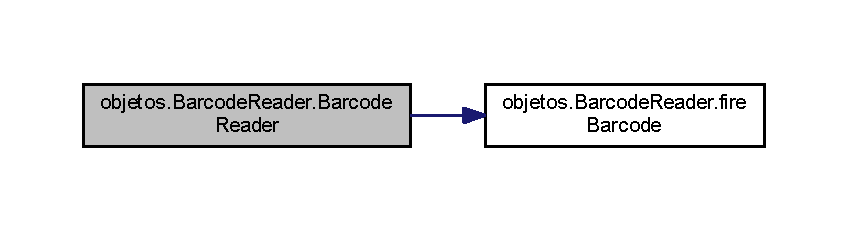
\includegraphics[width=350pt]{classobjetos_1_1_barcode_reader_a0dc943983b8313727f52c7e043805a80_cgraph}
\end{center}
\end{figure}


\subsection{Member Function Documentation}
\mbox{\Hypertarget{classobjetos_1_1_barcode_reader_a7c0a8f3e684c72a78005c97f3d9cdc24}\label{classobjetos_1_1_barcode_reader_a7c0a8f3e684c72a78005c97f3d9cdc24}} 
\index{objetos\+::\+Barcode\+Reader@{objetos\+::\+Barcode\+Reader}!add\+Barcode\+Listener@{add\+Barcode\+Listener}}
\index{add\+Barcode\+Listener@{add\+Barcode\+Listener}!objetos\+::\+Barcode\+Reader@{objetos\+::\+Barcode\+Reader}}
\subsubsection{\texorpdfstring{add\+Barcode\+Listener()}{addBarcodeListener()}}
{\footnotesize\ttfamily void objetos.\+Barcode\+Reader.\+add\+Barcode\+Listener (\begin{DoxyParamCaption}\item[{\mbox{\hyperlink{interfaceobjetos_1_1_barcode_reader_1_1_barcode_listener}{Barcode\+Listener}}}]{listener }\end{DoxyParamCaption})}



Definition at line 66 of file Barcode\+Reader.\+java.

\mbox{\Hypertarget{classobjetos_1_1_barcode_reader_a1cd53567cad388b796e540c7a9240bf7}\label{classobjetos_1_1_barcode_reader_a1cd53567cad388b796e540c7a9240bf7}} 
\index{objetos\+::\+Barcode\+Reader@{objetos\+::\+Barcode\+Reader}!fire\+Barcode@{fire\+Barcode}}
\index{fire\+Barcode@{fire\+Barcode}!objetos\+::\+Barcode\+Reader@{objetos\+::\+Barcode\+Reader}}
\subsubsection{\texorpdfstring{fire\+Barcode()}{fireBarcode()}}
{\footnotesize\ttfamily void objetos.\+Barcode\+Reader.\+fire\+Barcode (\begin{DoxyParamCaption}\item[{String}]{barcode }\end{DoxyParamCaption})\hspace{0.3cm}{\ttfamily [protected]}}



Definition at line 60 of file Barcode\+Reader.\+java.

\mbox{\Hypertarget{classobjetos_1_1_barcode_reader_a4b49668d25796160e591b78b89b287eb}\label{classobjetos_1_1_barcode_reader_a4b49668d25796160e591b78b89b287eb}} 
\index{objetos\+::\+Barcode\+Reader@{objetos\+::\+Barcode\+Reader}!remove\+Barcode\+Listener@{remove\+Barcode\+Listener}}
\index{remove\+Barcode\+Listener@{remove\+Barcode\+Listener}!objetos\+::\+Barcode\+Reader@{objetos\+::\+Barcode\+Reader}}
\subsubsection{\texorpdfstring{remove\+Barcode\+Listener()}{removeBarcodeListener()}}
{\footnotesize\ttfamily void objetos.\+Barcode\+Reader.\+remove\+Barcode\+Listener (\begin{DoxyParamCaption}\item[{\mbox{\hyperlink{interfaceobjetos_1_1_barcode_reader_1_1_barcode_listener}{Barcode\+Listener}}}]{listener }\end{DoxyParamCaption})}



Definition at line 70 of file Barcode\+Reader.\+java.



The documentation for this class was generated from the following file\+:\begin{DoxyCompactItemize}
\item 
C\+:/\+Users/jonmu/\+Desktop/\+P\+O\+P\+B\+L 4/src/objetos/\mbox{\hyperlink{_barcode_reader_8java}{Barcode\+Reader.\+java}}\end{DoxyCompactItemize}

\hypertarget{classmysql_1_1_conexion_j_d_b_c}{}\section{mysql.\+Conexion\+J\+D\+BC Class Reference}
\label{classmysql_1_1_conexion_j_d_b_c}\index{mysql.\+Conexion\+J\+D\+BC@{mysql.\+Conexion\+J\+D\+BC}}


Collaboration diagram for mysql.\+Conexion\+J\+D\+BC\+:
% FIG 0
\subsection*{Public Member Functions}
\begin{DoxyCompactItemize}
\item 
\mbox{\Hypertarget{classmysql_1_1_conexion_j_d_b_c_a342d326d6f6c9831bb117afccb912a04}\label{classmysql_1_1_conexion_j_d_b_c_a342d326d6f6c9831bb117afccb912a04}} 
Prepared\+Statement {\bfseries prepared\+Statement} (String sql)
\item 
\mbox{\Hypertarget{classmysql_1_1_conexion_j_d_b_c_a77f0c70a90a3e174114586b131f10909}\label{classmysql_1_1_conexion_j_d_b_c_a77f0c70a90a3e174114586b131f10909}} 
Result\+Set {\bfseries select} (String query)
\item 
\mbox{\Hypertarget{classmysql_1_1_conexion_j_d_b_c_a5a0abe91b83748401d0a630817c15e83}\label{classmysql_1_1_conexion_j_d_b_c_a5a0abe91b83748401d0a630817c15e83}} 
int {\bfseries update} (String query)
\item 
\mbox{\Hypertarget{classmysql_1_1_conexion_j_d_b_c_a7cb683b19298ad4ccda2ef51abb68302}\label{classmysql_1_1_conexion_j_d_b_c_a7cb683b19298ad4ccda2ef51abb68302}} 
int {\bfseries delete} (String query)
\item 
\mbox{\Hypertarget{classmysql_1_1_conexion_j_d_b_c_a05e552aeb511582e81c6dd6cba120182}\label{classmysql_1_1_conexion_j_d_b_c_a05e552aeb511582e81c6dd6cba120182}} 
void {\bfseries close} ()
\item 
\mbox{\Hypertarget{classmysql_1_1_conexion_j_d_b_c_a6d8f0cd0e2046952d9771d379c16562a}\label{classmysql_1_1_conexion_j_d_b_c_a6d8f0cd0e2046952d9771d379c16562a}} 
void {\bfseries registrar\+Pedido} (\mbox{\hyperlink{classobjetos_1_1_pedido}{Pedido}} p)
\item 
\mbox{\Hypertarget{classmysql_1_1_conexion_j_d_b_c_ab41e6e25d89ab9a807e9729fcdf5818f}\label{classmysql_1_1_conexion_j_d_b_c_ab41e6e25d89ab9a807e9729fcdf5818f}} 
void {\bfseries registrar\+Linea} (int pedido\+Id, int producto\+ID, double precio\+Producto, int cantidad\+Productos)
\item 
\mbox{\Hypertarget{classmysql_1_1_conexion_j_d_b_c_abbadbe682819495c2b2afd962afba245}\label{classmysql_1_1_conexion_j_d_b_c_abbadbe682819495c2b2afd962afba245}} 
int {\bfseries get\+Id\+Ultimo\+Pedido} ()  throws Class\+Not\+Found\+Exception, S\+Q\+L\+Exception 
\item 
\mbox{\Hypertarget{classmysql_1_1_conexion_j_d_b_c_a4dde03f79391c9a52f7a84e281c5a696}\label{classmysql_1_1_conexion_j_d_b_c_a4dde03f79391c9a52f7a84e281c5a696}} 
int {\bfseries get\+Id\+Usuario} (String usuario)  throws Class\+Not\+Found\+Exception, S\+Q\+L\+Exception 
\item 
\mbox{\Hypertarget{classmysql_1_1_conexion_j_d_b_c_afa9f004689cee7a90e6a19c359409e04}\label{classmysql_1_1_conexion_j_d_b_c_afa9f004689cee7a90e6a19c359409e04}} 
Array\+List$<$ \mbox{\hyperlink{classobjetos_1_1_usuario}{Usuario}} $>$ {\bfseries get\+Lista\+Usuarios} ()  throws Class\+Not\+Found\+Exception, S\+Q\+L\+Exception 
\item 
\mbox{\Hypertarget{classmysql_1_1_conexion_j_d_b_c_a38333a2f31d016faaf14c08901c6ffea}\label{classmysql_1_1_conexion_j_d_b_c_a38333a2f31d016faaf14c08901c6ffea}} 
Array\+List$<$ \mbox{\hyperlink{classobjetos_1_1_pedido}{Pedido}} $>$ {\bfseries get\+Lista\+Pedidos} (String usuario)  throws Class\+Not\+Found\+Exception, S\+Q\+L\+Exception 
\item 
\mbox{\Hypertarget{classmysql_1_1_conexion_j_d_b_c_a93e878bd79640edb42bbaa5e11217f8e}\label{classmysql_1_1_conexion_j_d_b_c_a93e878bd79640edb42bbaa5e11217f8e}} 
Array\+List$<$ \mbox{\hyperlink{classobjetos_1_1_producto}{Producto}} $>$ {\bfseries get\+Lista\+Productos} (int pedido\+ID)  throws Class\+Not\+Found\+Exception, S\+Q\+L\+Exception 
\item 
\mbox{\Hypertarget{classmysql_1_1_conexion_j_d_b_c_a5dbbd093ae378b5b023127bdf0ccf88e}\label{classmysql_1_1_conexion_j_d_b_c_a5dbbd093ae378b5b023127bdf0ccf88e}} 
void {\bfseries guardar\+Pedidos\+BD} (\mbox{\hyperlink{classobjetos_1_1_usuario}{Usuario}} u)
\end{DoxyCompactItemize}


The documentation for this class was generated from the following file\+:\begin{DoxyCompactItemize}
\item 
C\+:/\+Users/jonmu/\+Desktop/\+P\+O\+P\+B\+L 4/src/mysql/Conexion\+J\+D\+B\+C.\+java\end{DoxyCompactItemize}

\hypertarget{classcontroladores_1_1_controlador_acceso}{}\section{controladores.\+Controlador\+Acceso Class Reference}
\label{classcontroladores_1_1_controlador_acceso}\index{controladores.\+Controlador\+Acceso@{controladores.\+Controlador\+Acceso}}


Inheritance diagram for controladores.\+Controlador\+Acceso\+:
\nopagebreak
\begin{figure}[H]
\begin{center}
\leavevmode
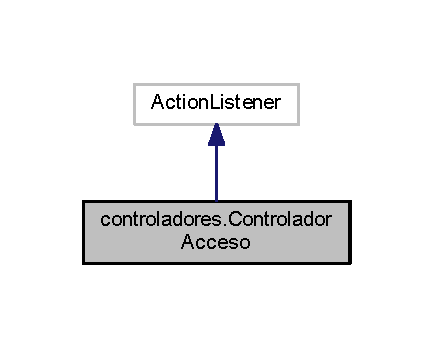
\includegraphics[width=208pt]{classcontroladores_1_1_controlador_acceso__inherit__graph}
\end{center}
\end{figure}


Collaboration diagram for controladores.\+Controlador\+Acceso\+:
\nopagebreak
\begin{figure}[H]
\begin{center}
\leavevmode
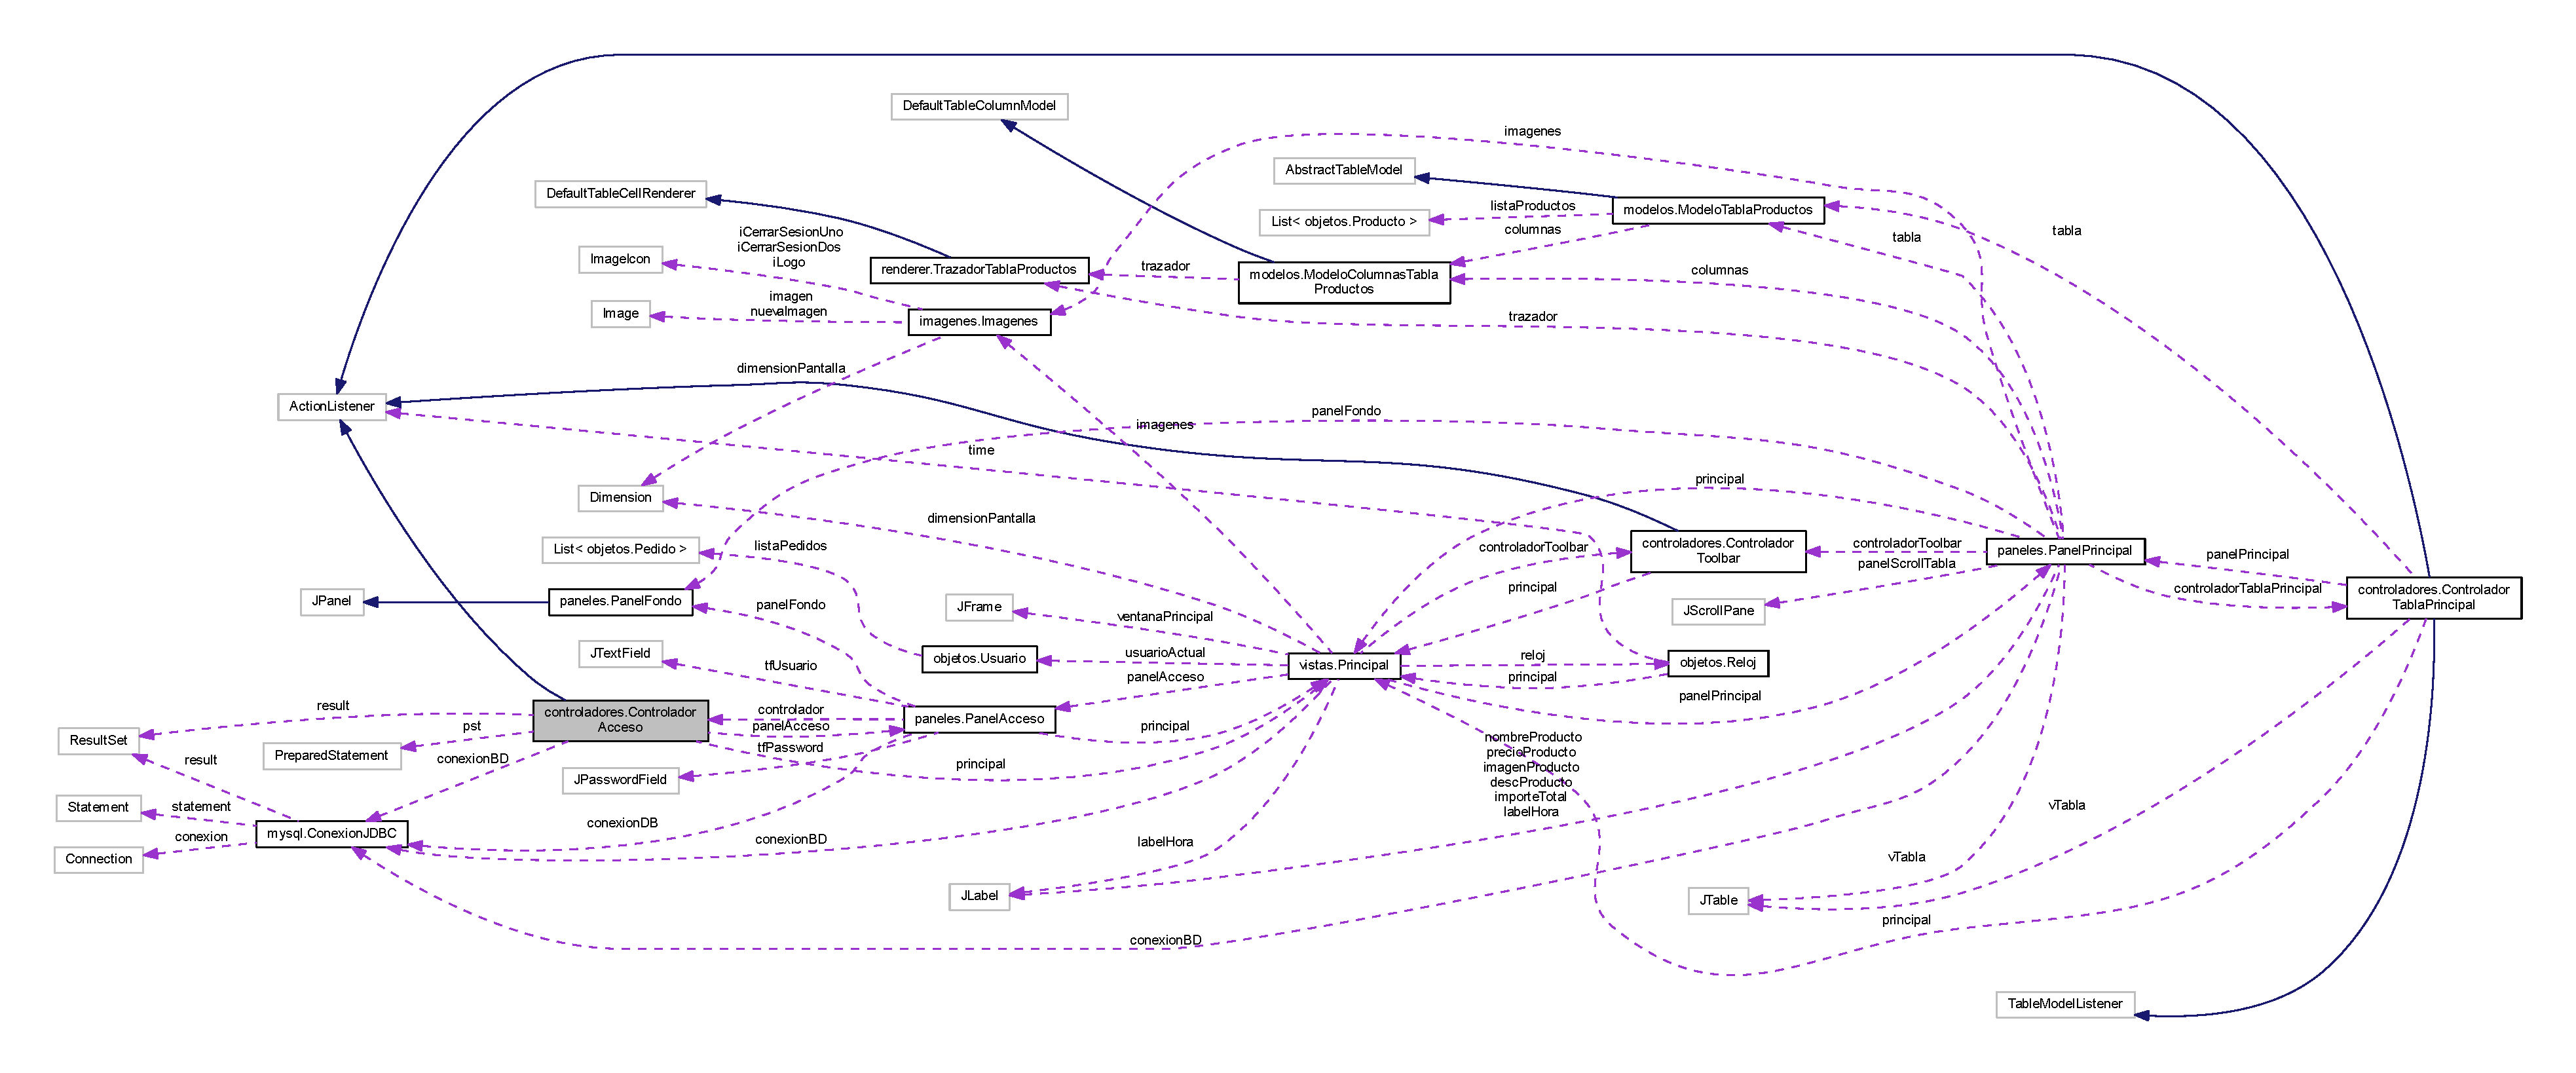
\includegraphics[width=350pt]{classcontroladores_1_1_controlador_acceso__coll__graph}
\end{center}
\end{figure}
\subsection*{Public Member Functions}
\begin{DoxyCompactItemize}
\item 
\mbox{\hyperlink{classcontroladores_1_1_controlador_acceso_ac9e7e1075d18fe14a6eb23ebcfb7b169}{Controlador\+Acceso}} (\mbox{\hyperlink{classpaneles_1_1_panel_acceso}{Panel\+Acceso}} panel\+Acceso, \mbox{\hyperlink{classmysql_1_1_conexion_j_d_b_c}{Conexion\+J\+D\+BC}} conexion\+BD, \mbox{\hyperlink{classvistas_1_1_principal}{Principal}} principal)
\item 
void \mbox{\hyperlink{classcontroladores_1_1_controlador_acceso_ab61e9c919427421412501af1772a005a}{action\+Performed}} (Action\+Event e)
\item 
String \mbox{\hyperlink{classcontroladores_1_1_controlador_acceso_a935597b08e48ed6c762ee91ad7e0f5ea}{md5}} (String pass)
\end{DoxyCompactItemize}


\subsection{Detailed Description}


Definition at line 19 of file Controlador\+Acceso.\+java.



\subsection{Constructor \& Destructor Documentation}
\mbox{\Hypertarget{classcontroladores_1_1_controlador_acceso_ac9e7e1075d18fe14a6eb23ebcfb7b169}\label{classcontroladores_1_1_controlador_acceso_ac9e7e1075d18fe14a6eb23ebcfb7b169}} 
\index{controladores\+::\+Controlador\+Acceso@{controladores\+::\+Controlador\+Acceso}!Controlador\+Acceso@{Controlador\+Acceso}}
\index{Controlador\+Acceso@{Controlador\+Acceso}!controladores\+::\+Controlador\+Acceso@{controladores\+::\+Controlador\+Acceso}}
\subsubsection{\texorpdfstring{Controlador\+Acceso()}{ControladorAcceso()}}
{\footnotesize\ttfamily controladores.\+Controlador\+Acceso.\+Controlador\+Acceso (\begin{DoxyParamCaption}\item[{\mbox{\hyperlink{classpaneles_1_1_panel_acceso}{Panel\+Acceso}}}]{panel\+Acceso,  }\item[{\mbox{\hyperlink{classmysql_1_1_conexion_j_d_b_c}{Conexion\+J\+D\+BC}}}]{conexion\+BD,  }\item[{\mbox{\hyperlink{classvistas_1_1_principal}{Principal}}}]{principal }\end{DoxyParamCaption})}



Definition at line 28 of file Controlador\+Acceso.\+java.



\subsection{Member Function Documentation}
\mbox{\Hypertarget{classcontroladores_1_1_controlador_acceso_ab61e9c919427421412501af1772a005a}\label{classcontroladores_1_1_controlador_acceso_ab61e9c919427421412501af1772a005a}} 
\index{controladores\+::\+Controlador\+Acceso@{controladores\+::\+Controlador\+Acceso}!action\+Performed@{action\+Performed}}
\index{action\+Performed@{action\+Performed}!controladores\+::\+Controlador\+Acceso@{controladores\+::\+Controlador\+Acceso}}
\subsubsection{\texorpdfstring{action\+Performed()}{actionPerformed()}}
{\footnotesize\ttfamily void controladores.\+Controlador\+Acceso.\+action\+Performed (\begin{DoxyParamCaption}\item[{Action\+Event}]{e }\end{DoxyParamCaption})}



Definition at line 35 of file Controlador\+Acceso.\+java.

Here is the call graph for this function\+:
\nopagebreak
\begin{figure}[H]
\begin{center}
\leavevmode
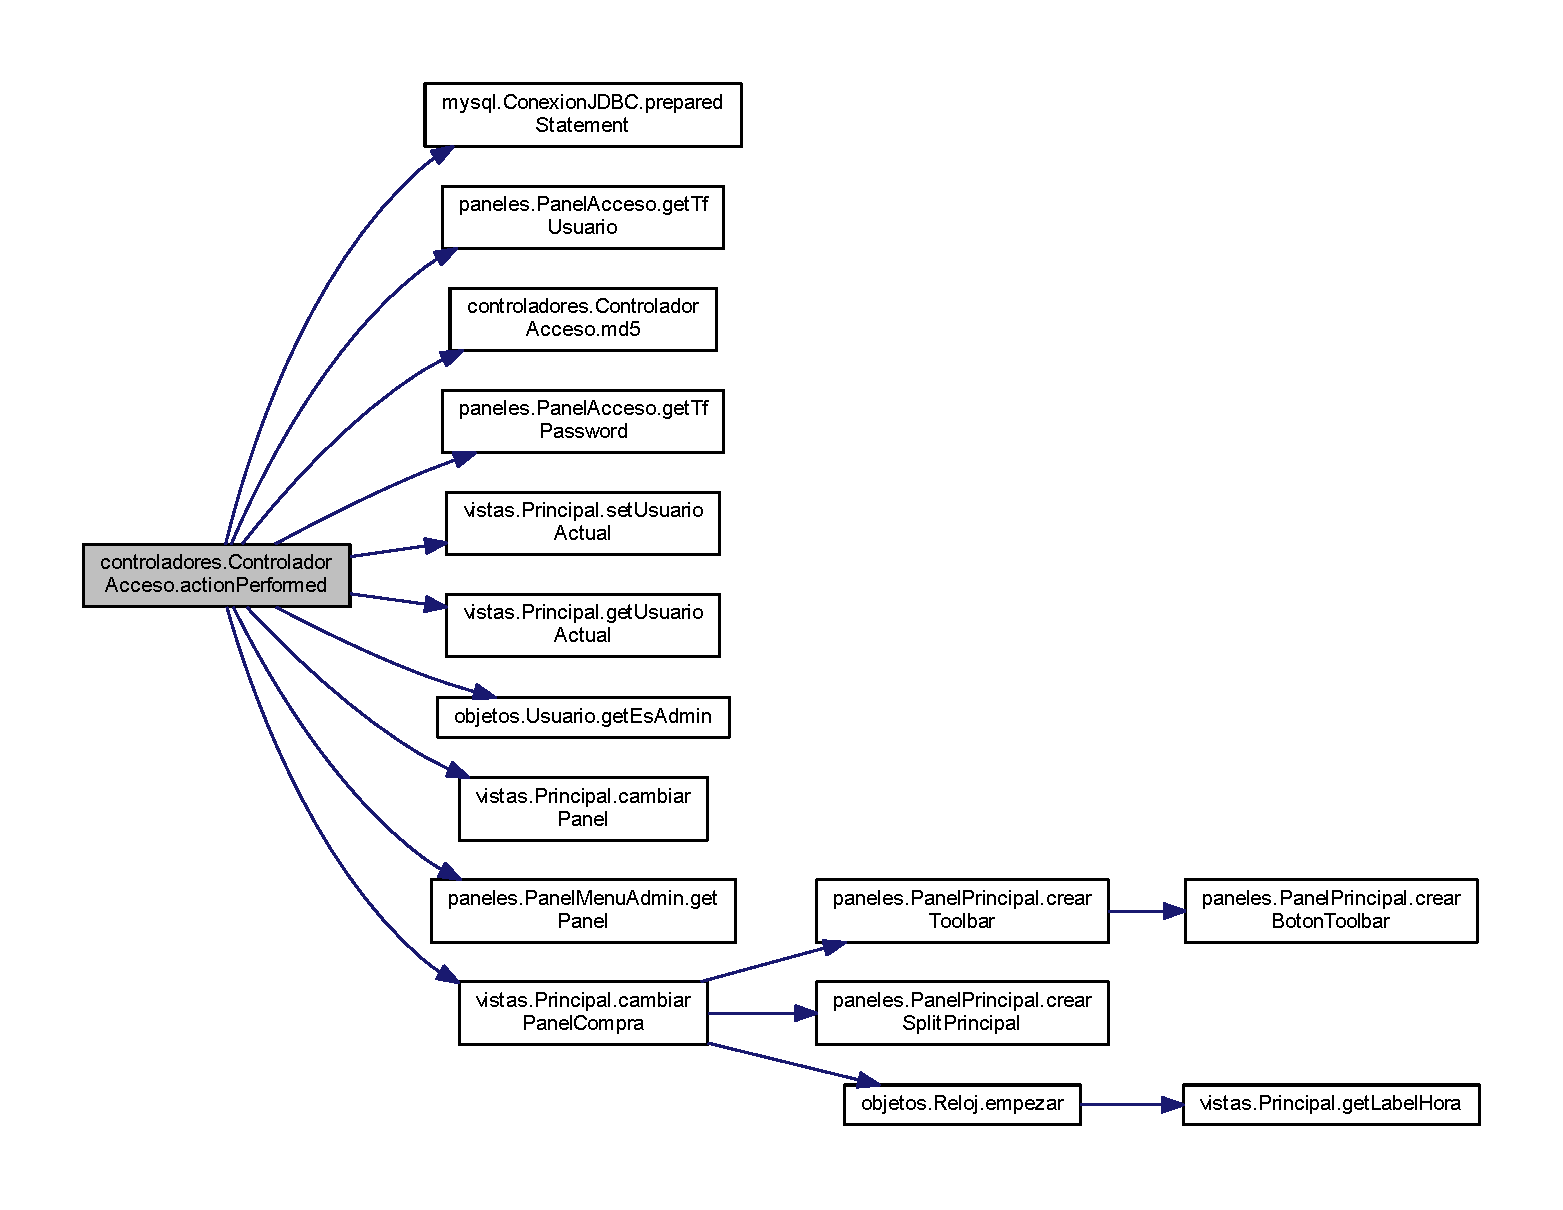
\includegraphics[width=350pt]{classcontroladores_1_1_controlador_acceso_ab61e9c919427421412501af1772a005a_cgraph}
\end{center}
\end{figure}
\mbox{\Hypertarget{classcontroladores_1_1_controlador_acceso_a935597b08e48ed6c762ee91ad7e0f5ea}\label{classcontroladores_1_1_controlador_acceso_a935597b08e48ed6c762ee91ad7e0f5ea}} 
\index{controladores\+::\+Controlador\+Acceso@{controladores\+::\+Controlador\+Acceso}!md5@{md5}}
\index{md5@{md5}!controladores\+::\+Controlador\+Acceso@{controladores\+::\+Controlador\+Acceso}}
\subsubsection{\texorpdfstring{md5()}{md5()}}
{\footnotesize\ttfamily String controladores.\+Controlador\+Acceso.\+md5 (\begin{DoxyParamCaption}\item[{String}]{pass }\end{DoxyParamCaption})}



Definition at line 80 of file Controlador\+Acceso.\+java.



The documentation for this class was generated from the following file\+:\begin{DoxyCompactItemize}
\item 
C\+:/\+Users/jonmu/\+Desktop/\+P\+O\+P\+B\+L 4/src/controladores/\mbox{\hyperlink{_controlador_acceso_8java}{Controlador\+Acceso.\+java}}\end{DoxyCompactItemize}

\hypertarget{classcontroladores_1_1_controlador_menu_admin}{}\section{controladores.\+Controlador\+Menu\+Admin Class Reference}
\label{classcontroladores_1_1_controlador_menu_admin}\index{controladores.\+Controlador\+Menu\+Admin@{controladores.\+Controlador\+Menu\+Admin}}


Inheritance diagram for controladores.\+Controlador\+Menu\+Admin\+:\nopagebreak
\begin{figure}[H]
\begin{center}
\leavevmode
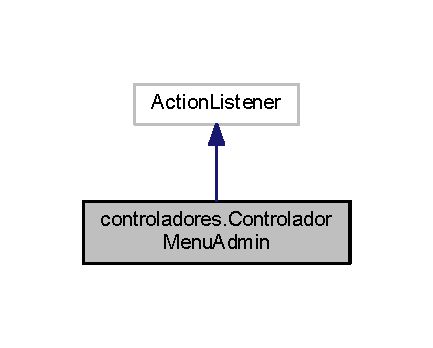
\includegraphics[width=208pt]{classcontroladores_1_1_controlador_menu_admin__inherit__graph}
\end{center}
\end{figure}


Collaboration diagram for controladores.\+Controlador\+Menu\+Admin\+:\nopagebreak
\begin{figure}[H]
\begin{center}
\leavevmode
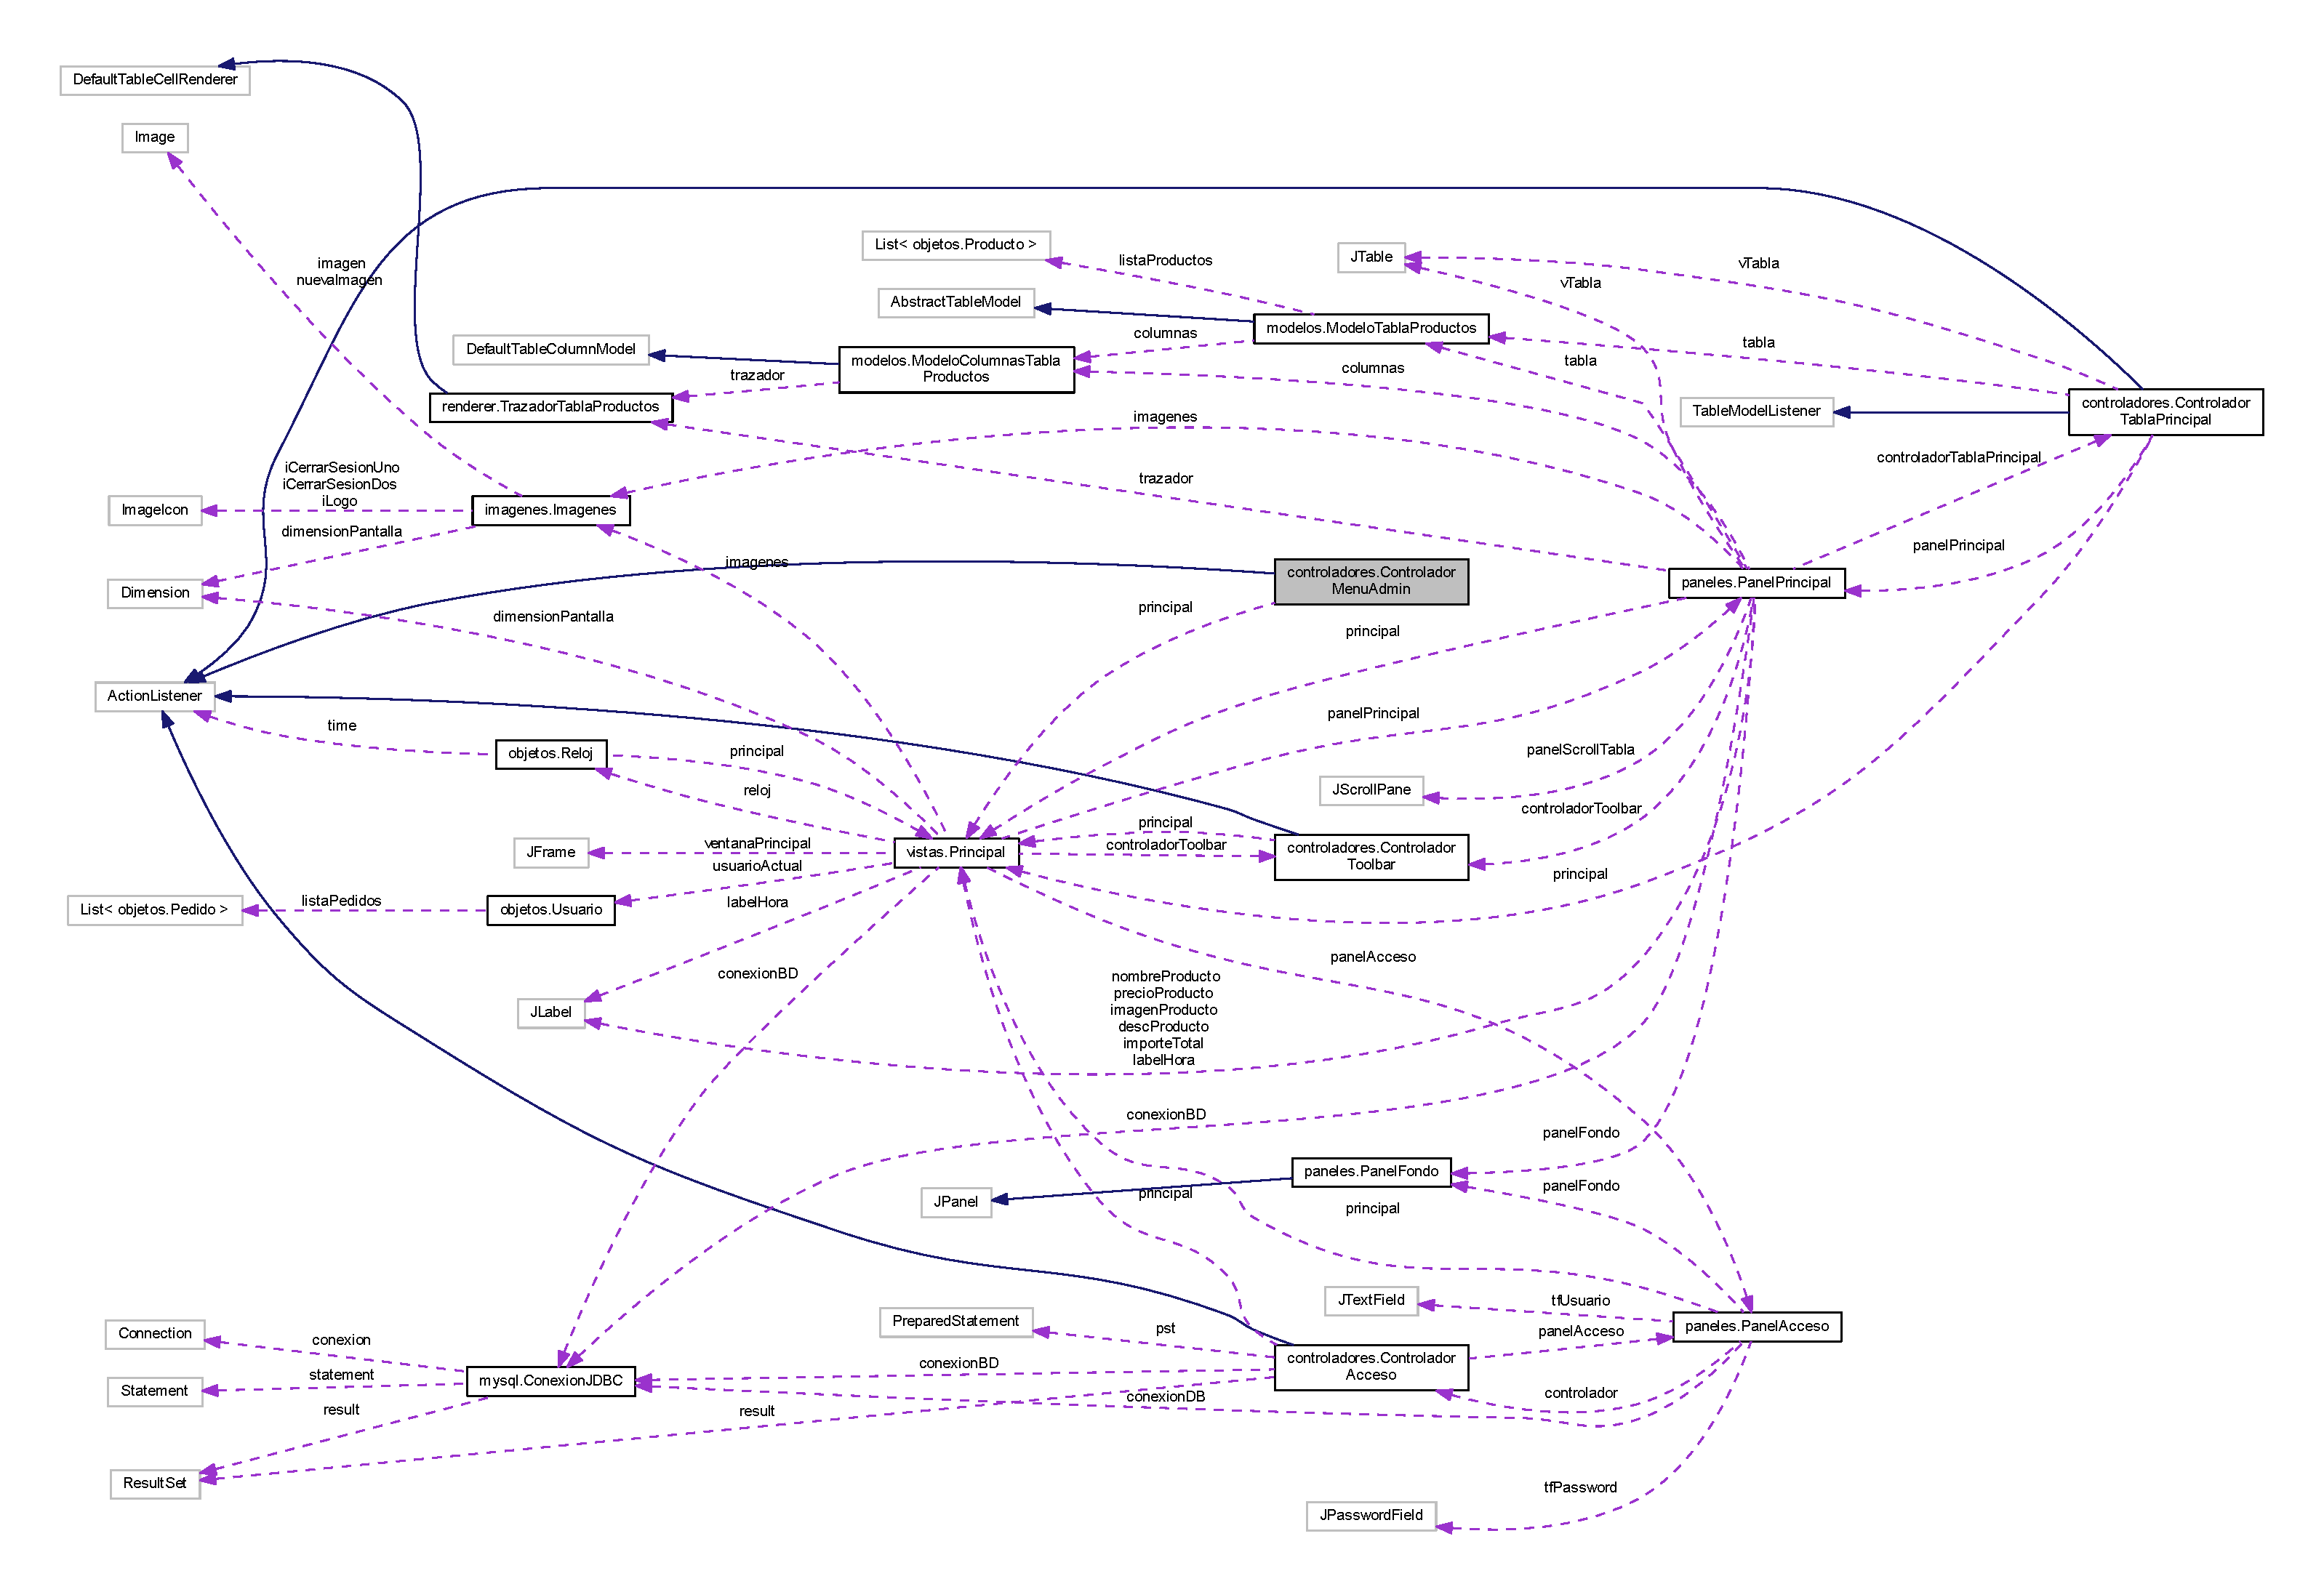
\includegraphics[width=350pt]{classcontroladores_1_1_controlador_menu_admin__coll__graph}
\end{center}
\end{figure}
\subsection*{Public Member Functions}
\begin{DoxyCompactItemize}
\item 
\mbox{\hyperlink{classcontroladores_1_1_controlador_menu_admin_a12c2b360472a2aa24c7ca77751a3880c}{Controlador\+Menu\+Admin}} (\mbox{\hyperlink{classvistas_1_1_principal}{Principal}} principal)
\item 
void \mbox{\hyperlink{classcontroladores_1_1_controlador_menu_admin_a82d2cd7e031a45484fdf83e50a82cf1e}{action\+Performed}} (Action\+Event e)
\end{DoxyCompactItemize}


\subsection{Detailed Description}


Definition at line 13 of file Controlador\+Menu\+Admin.\+java.



\subsection{Constructor \& Destructor Documentation}
\mbox{\Hypertarget{classcontroladores_1_1_controlador_menu_admin_a12c2b360472a2aa24c7ca77751a3880c}\label{classcontroladores_1_1_controlador_menu_admin_a12c2b360472a2aa24c7ca77751a3880c}} 
\index{controladores\+::\+Controlador\+Menu\+Admin@{controladores\+::\+Controlador\+Menu\+Admin}!Controlador\+Menu\+Admin@{Controlador\+Menu\+Admin}}
\index{Controlador\+Menu\+Admin@{Controlador\+Menu\+Admin}!controladores\+::\+Controlador\+Menu\+Admin@{controladores\+::\+Controlador\+Menu\+Admin}}
\subsubsection{\texorpdfstring{Controlador\+Menu\+Admin()}{ControladorMenuAdmin()}}
{\footnotesize\ttfamily controladores.\+Controlador\+Menu\+Admin.\+Controlador\+Menu\+Admin (\begin{DoxyParamCaption}\item[{\mbox{\hyperlink{classvistas_1_1_principal}{Principal}}}]{principal }\end{DoxyParamCaption})}



Definition at line 17 of file Controlador\+Menu\+Admin.\+java.



\subsection{Member Function Documentation}
\mbox{\Hypertarget{classcontroladores_1_1_controlador_menu_admin_a82d2cd7e031a45484fdf83e50a82cf1e}\label{classcontroladores_1_1_controlador_menu_admin_a82d2cd7e031a45484fdf83e50a82cf1e}} 
\index{controladores\+::\+Controlador\+Menu\+Admin@{controladores\+::\+Controlador\+Menu\+Admin}!action\+Performed@{action\+Performed}}
\index{action\+Performed@{action\+Performed}!controladores\+::\+Controlador\+Menu\+Admin@{controladores\+::\+Controlador\+Menu\+Admin}}
\subsubsection{\texorpdfstring{action\+Performed()}{actionPerformed()}}
{\footnotesize\ttfamily void controladores.\+Controlador\+Menu\+Admin.\+action\+Performed (\begin{DoxyParamCaption}\item[{Action\+Event}]{e }\end{DoxyParamCaption})}



Definition at line 22 of file Controlador\+Menu\+Admin.\+java.

Here is the call graph for this function\+:\nopagebreak
\begin{figure}[H]
\begin{center}
\leavevmode
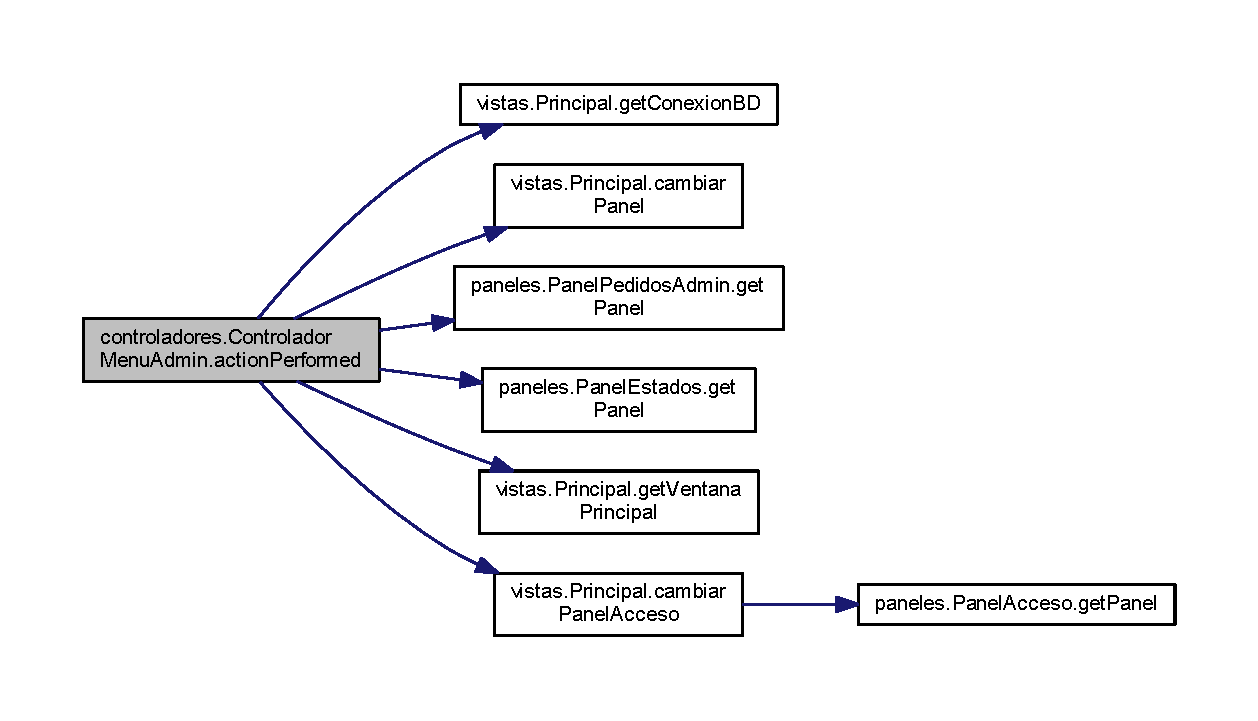
\includegraphics[width=350pt]{classcontroladores_1_1_controlador_menu_admin_a82d2cd7e031a45484fdf83e50a82cf1e_cgraph}
\end{center}
\end{figure}


The documentation for this class was generated from the following file\+:\begin{DoxyCompactItemize}
\item 
C\+:/\+Users/jonmu/\+Desktop/\+P\+O\+P\+B\+L 4/src/controladores/\mbox{\hyperlink{_controlador_menu_admin_8java}{Controlador\+Menu\+Admin.\+java}}\end{DoxyCompactItemize}

\hypertarget{classcontroladores_1_1_controlador_tabla_principal}{}\section{controladores.\+Controlador\+Tabla\+Principal Class Reference}
\label{classcontroladores_1_1_controlador_tabla_principal}\index{controladores.\+Controlador\+Tabla\+Principal@{controladores.\+Controlador\+Tabla\+Principal}}


Inheritance diagram for controladores.\+Controlador\+Tabla\+Principal\+:
\nopagebreak
\begin{figure}[H]
\begin{center}
\leavevmode
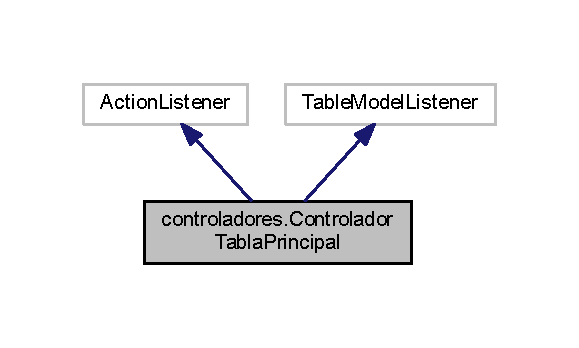
\includegraphics[width=278pt]{classcontroladores_1_1_controlador_tabla_principal__inherit__graph}
\end{center}
\end{figure}


Collaboration diagram for controladores.\+Controlador\+Tabla\+Principal\+:
\nopagebreak
\begin{figure}[H]
\begin{center}
\leavevmode
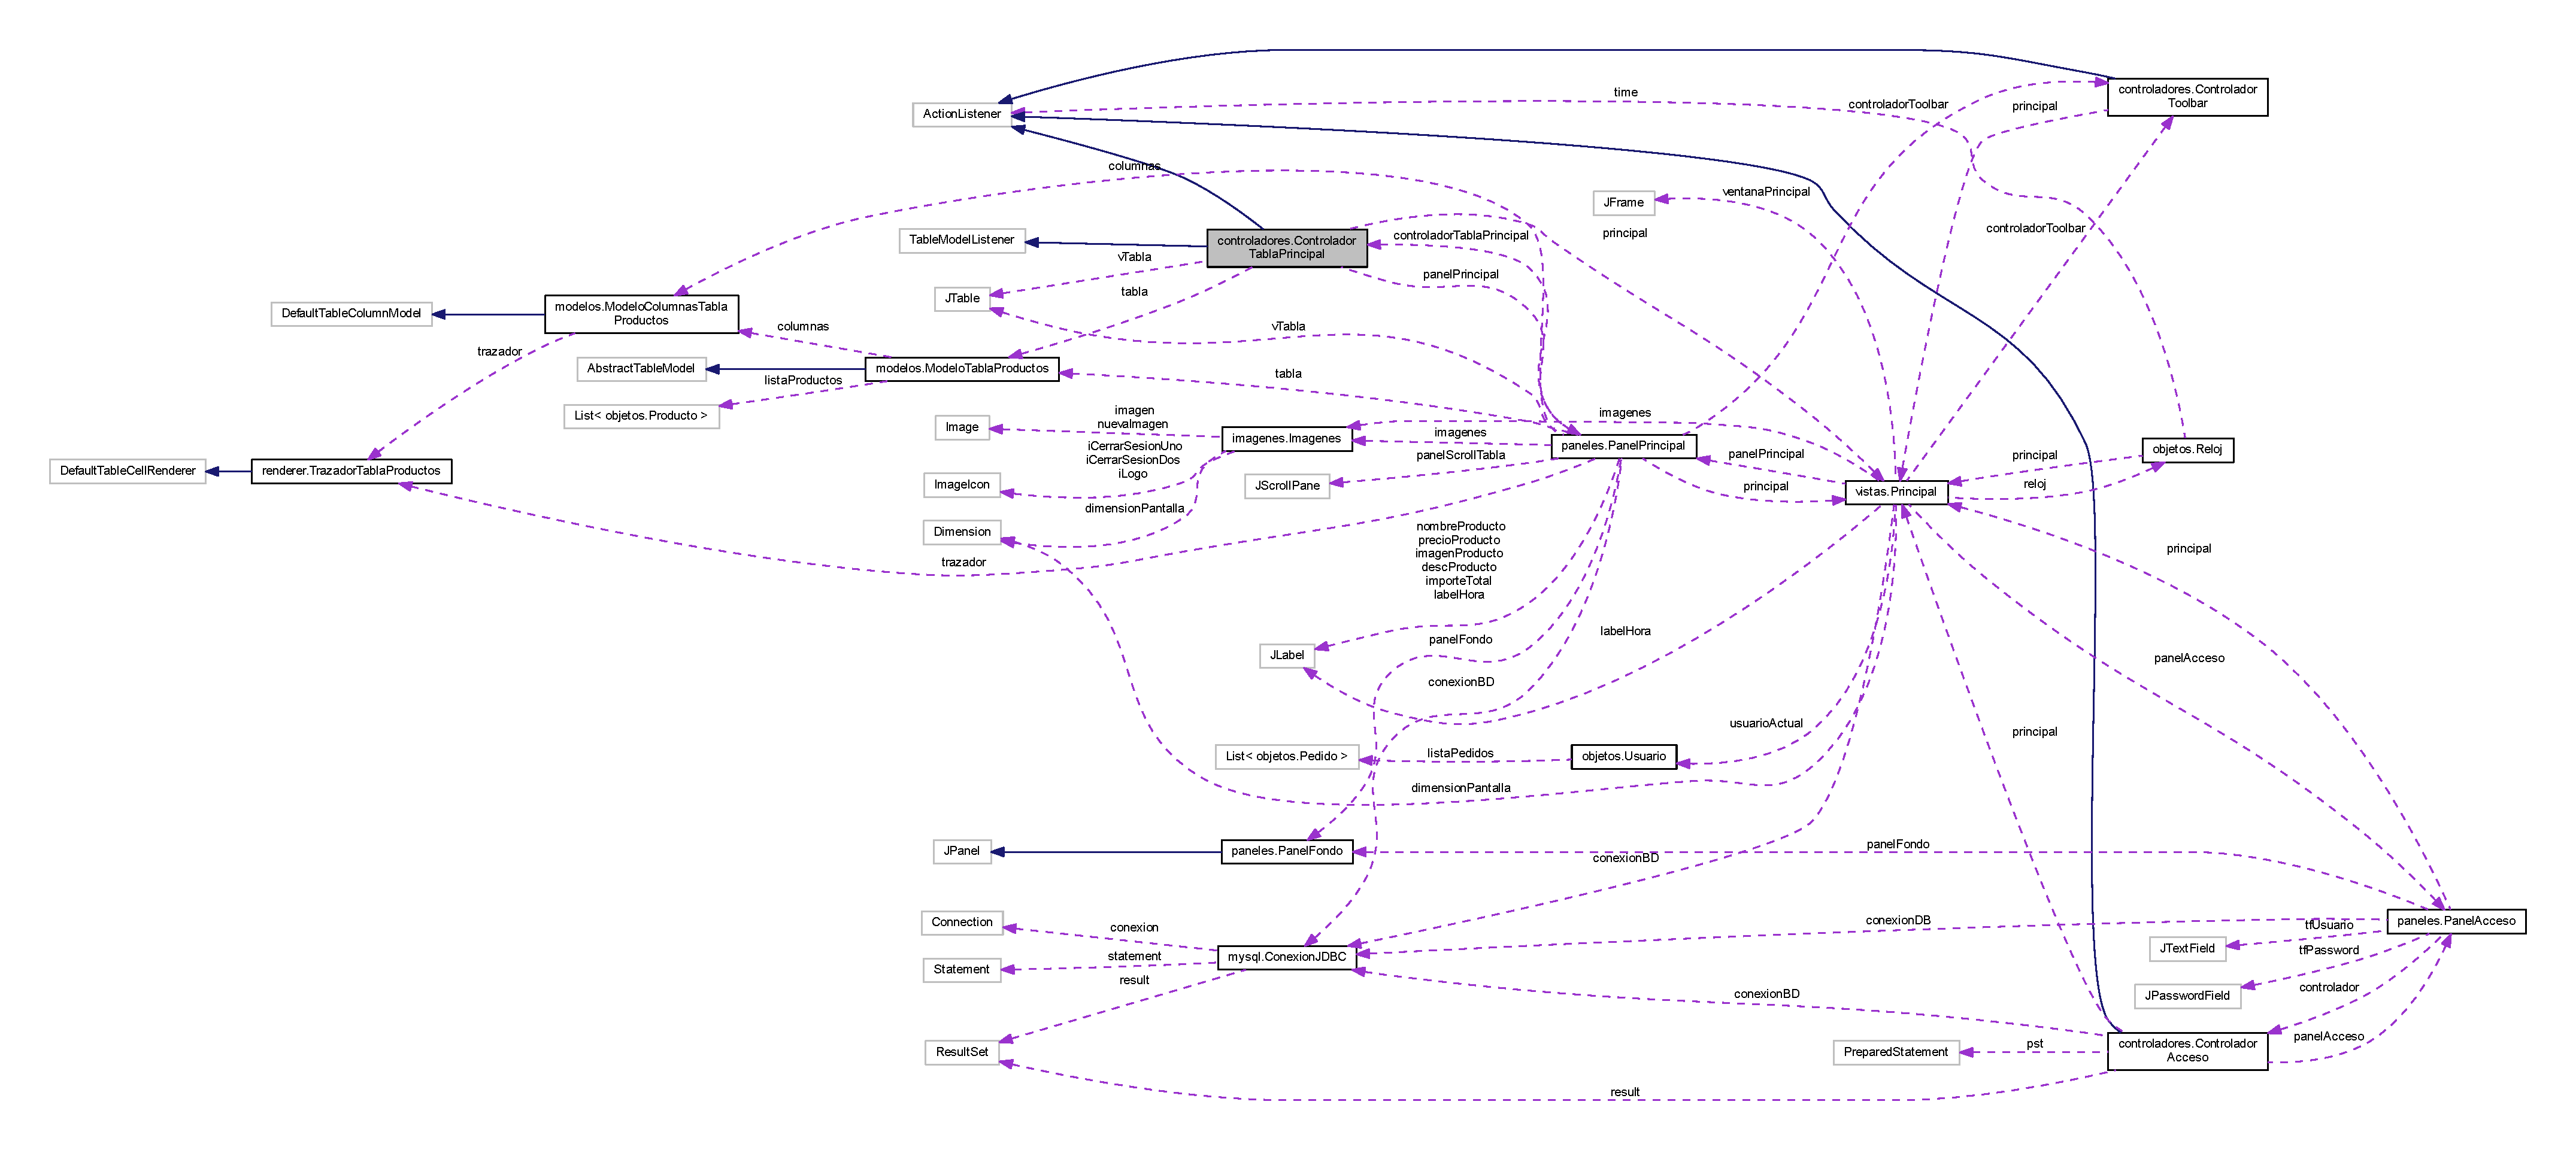
\includegraphics[width=350pt]{classcontroladores_1_1_controlador_tabla_principal__coll__graph}
\end{center}
\end{figure}
\subsection*{Public Member Functions}
\begin{DoxyCompactItemize}
\item 
\mbox{\hyperlink{classcontroladores_1_1_controlador_tabla_principal_a279325fa05462ea55845646a812d9a84}{Controlador\+Tabla\+Principal}} (\mbox{\hyperlink{classvistas_1_1_principal}{Principal}} principal, \mbox{\hyperlink{classmodelos_1_1_modelo_tabla_productos}{Modelo\+Tabla\+Productos}} tabla, J\+Table v\+Tabla, \mbox{\hyperlink{classpaneles_1_1_panel_principal}{Panel\+Principal}} panel\+Principal)
\item 
void \mbox{\hyperlink{classcontroladores_1_1_controlador_tabla_principal_a7ccd2cb9c153dbdd5d572be6d7a7aa5f}{action\+Performed}} (Action\+Event e)
\item 
void \mbox{\hyperlink{classcontroladores_1_1_controlador_tabla_principal_af223db673a317026cd0ce727b661fdea}{table\+Changed}} (Table\+Model\+Event e)
\end{DoxyCompactItemize}


\subsection{Detailed Description}


Definition at line 14 of file Controlador\+Tabla\+Principal.\+java.



\subsection{Constructor \& Destructor Documentation}
\mbox{\Hypertarget{classcontroladores_1_1_controlador_tabla_principal_a279325fa05462ea55845646a812d9a84}\label{classcontroladores_1_1_controlador_tabla_principal_a279325fa05462ea55845646a812d9a84}} 
\index{controladores\+::\+Controlador\+Tabla\+Principal@{controladores\+::\+Controlador\+Tabla\+Principal}!Controlador\+Tabla\+Principal@{Controlador\+Tabla\+Principal}}
\index{Controlador\+Tabla\+Principal@{Controlador\+Tabla\+Principal}!controladores\+::\+Controlador\+Tabla\+Principal@{controladores\+::\+Controlador\+Tabla\+Principal}}
\subsubsection{\texorpdfstring{Controlador\+Tabla\+Principal()}{ControladorTablaPrincipal()}}
{\footnotesize\ttfamily controladores.\+Controlador\+Tabla\+Principal.\+Controlador\+Tabla\+Principal (\begin{DoxyParamCaption}\item[{\mbox{\hyperlink{classvistas_1_1_principal}{Principal}}}]{principal,  }\item[{\mbox{\hyperlink{classmodelos_1_1_modelo_tabla_productos}{Modelo\+Tabla\+Productos}}}]{tabla,  }\item[{J\+Table}]{v\+Tabla,  }\item[{\mbox{\hyperlink{classpaneles_1_1_panel_principal}{Panel\+Principal}}}]{panel\+Principal }\end{DoxyParamCaption})}



Definition at line 21 of file Controlador\+Tabla\+Principal.\+java.



\subsection{Member Function Documentation}
\mbox{\Hypertarget{classcontroladores_1_1_controlador_tabla_principal_a7ccd2cb9c153dbdd5d572be6d7a7aa5f}\label{classcontroladores_1_1_controlador_tabla_principal_a7ccd2cb9c153dbdd5d572be6d7a7aa5f}} 
\index{controladores\+::\+Controlador\+Tabla\+Principal@{controladores\+::\+Controlador\+Tabla\+Principal}!action\+Performed@{action\+Performed}}
\index{action\+Performed@{action\+Performed}!controladores\+::\+Controlador\+Tabla\+Principal@{controladores\+::\+Controlador\+Tabla\+Principal}}
\subsubsection{\texorpdfstring{action\+Performed()}{actionPerformed()}}
{\footnotesize\ttfamily void controladores.\+Controlador\+Tabla\+Principal.\+action\+Performed (\begin{DoxyParamCaption}\item[{Action\+Event}]{e }\end{DoxyParamCaption})}



Definition at line 29 of file Controlador\+Tabla\+Principal.\+java.

Here is the call graph for this function\+:
\nopagebreak
\begin{figure}[H]
\begin{center}
\leavevmode
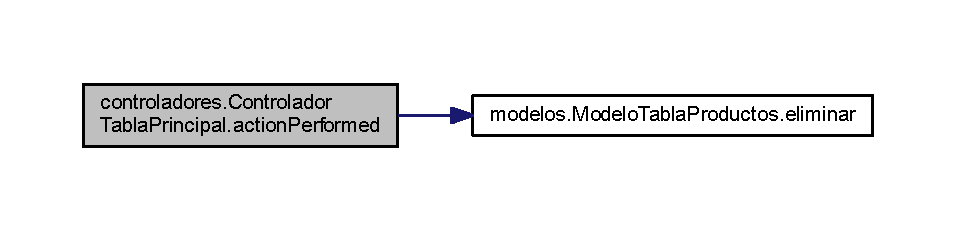
\includegraphics[width=350pt]{classcontroladores_1_1_controlador_tabla_principal_a7ccd2cb9c153dbdd5d572be6d7a7aa5f_cgraph}
\end{center}
\end{figure}
\mbox{\Hypertarget{classcontroladores_1_1_controlador_tabla_principal_af223db673a317026cd0ce727b661fdea}\label{classcontroladores_1_1_controlador_tabla_principal_af223db673a317026cd0ce727b661fdea}} 
\index{controladores\+::\+Controlador\+Tabla\+Principal@{controladores\+::\+Controlador\+Tabla\+Principal}!table\+Changed@{table\+Changed}}
\index{table\+Changed@{table\+Changed}!controladores\+::\+Controlador\+Tabla\+Principal@{controladores\+::\+Controlador\+Tabla\+Principal}}
\subsubsection{\texorpdfstring{table\+Changed()}{tableChanged()}}
{\footnotesize\ttfamily void controladores.\+Controlador\+Tabla\+Principal.\+table\+Changed (\begin{DoxyParamCaption}\item[{Table\+Model\+Event}]{e }\end{DoxyParamCaption})}



Definition at line 37 of file Controlador\+Tabla\+Principal.\+java.

Here is the call graph for this function\+:
\nopagebreak
\begin{figure}[H]
\begin{center}
\leavevmode
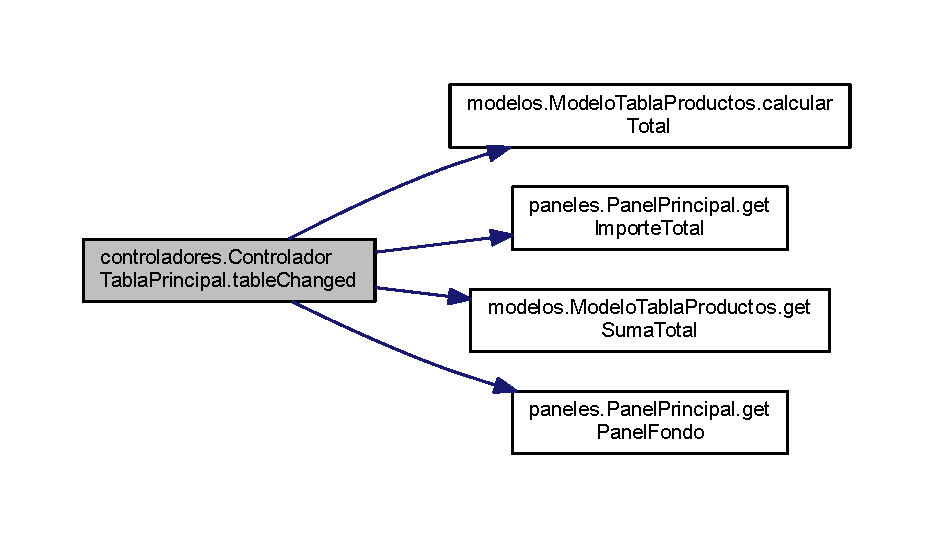
\includegraphics[width=350pt]{classcontroladores_1_1_controlador_tabla_principal_af223db673a317026cd0ce727b661fdea_cgraph}
\end{center}
\end{figure}


The documentation for this class was generated from the following file\+:\begin{DoxyCompactItemize}
\item 
C\+:/\+Users/jonmu/\+Desktop/\+P\+O\+P\+B\+L 4/src/controladores/\mbox{\hyperlink{_controlador_tabla_principal_8java}{Controlador\+Tabla\+Principal.\+java}}\end{DoxyCompactItemize}

\hypertarget{classcontroladores_1_1_controlador_toolbar}{}\section{controladores.\+Controlador\+Toolbar Class Reference}
\label{classcontroladores_1_1_controlador_toolbar}\index{controladores.\+Controlador\+Toolbar@{controladores.\+Controlador\+Toolbar}}


Inheritance diagram for controladores.\+Controlador\+Toolbar\+:
% FIG 0


Collaboration diagram for controladores.\+Controlador\+Toolbar\+:
% FIG 1
\subsection*{Public Member Functions}
\begin{DoxyCompactItemize}
\item 
\mbox{\Hypertarget{classcontroladores_1_1_controlador_toolbar_a7186864bd3fd61279fc13c4566d86cc3}\label{classcontroladores_1_1_controlador_toolbar_a7186864bd3fd61279fc13c4566d86cc3}} 
{\bfseries Controlador\+Toolbar} (\mbox{\hyperlink{classvistas_1_1_principal}{Principal}} principal)
\item 
\mbox{\Hypertarget{classcontroladores_1_1_controlador_toolbar_a21d7012349c1f101be2d87495da85fa6}\label{classcontroladores_1_1_controlador_toolbar_a21d7012349c1f101be2d87495da85fa6}} 
void {\bfseries action\+Performed} (Action\+Event e)
\end{DoxyCompactItemize}


The documentation for this class was generated from the following file\+:\begin{DoxyCompactItemize}
\item 
C\+:/\+Users/jonmu/\+Desktop/\+P\+O\+P\+B\+L 4/src/controladores/Controlador\+Toolbar.\+java\end{DoxyCompactItemize}

\hypertarget{classlineaserie_1_1_escritor}{}\section{lineaserie.\+Escritor Class Reference}
\label{classlineaserie_1_1_escritor}\index{lineaserie.\+Escritor@{lineaserie.\+Escritor}}


Inheritance diagram for lineaserie.\+Escritor\+:
\nopagebreak
\begin{figure}[H]
\begin{center}
\leavevmode
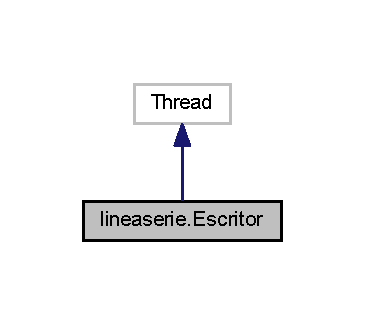
\includegraphics[width=175pt]{classlineaserie_1_1_escritor__inherit__graph}
\end{center}
\end{figure}


Collaboration diagram for lineaserie.\+Escritor\+:
\nopagebreak
\begin{figure}[H]
\begin{center}
\leavevmode
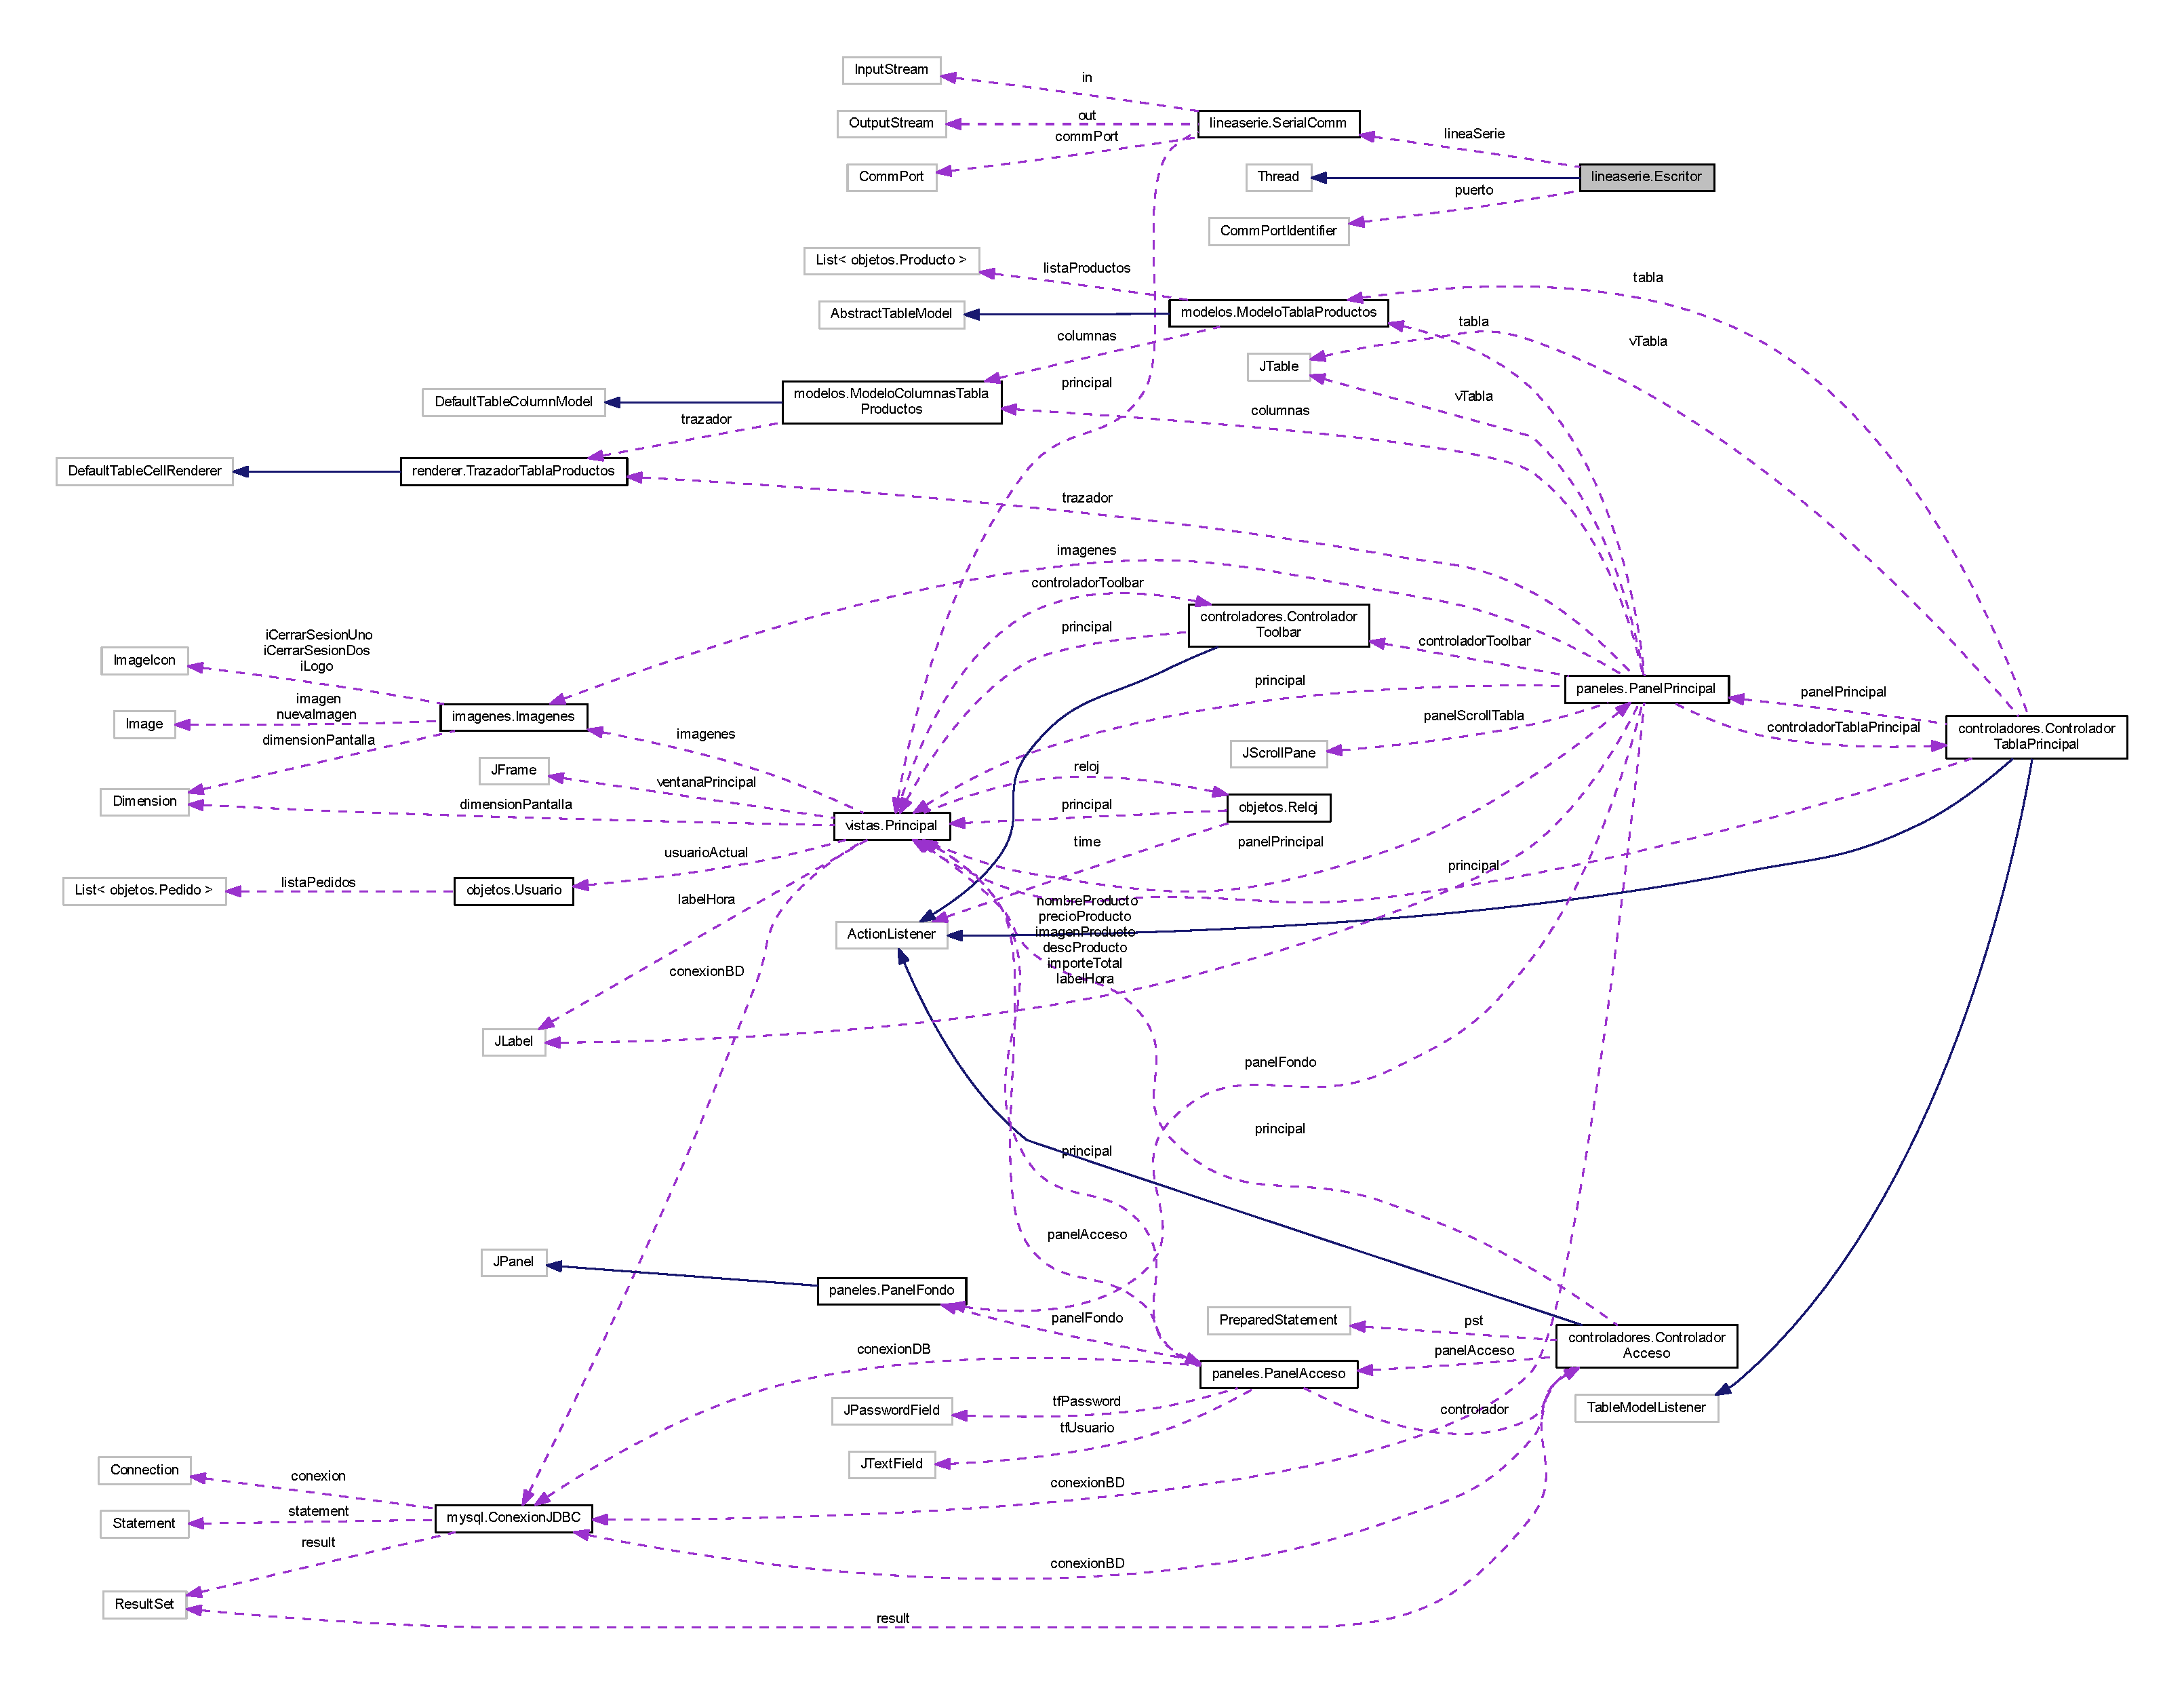
\includegraphics[width=350pt]{classlineaserie_1_1_escritor__coll__graph}
\end{center}
\end{figure}
\subsection*{Public Member Functions}
\begin{DoxyCompactItemize}
\item 
\mbox{\hyperlink{classlineaserie_1_1_escritor_a0469893e8a8e4548e89ead10694676db}{Escritor}} (\mbox{\hyperlink{classlineaserie_1_1_serial_comm}{Serial\+Comm}} linea\+Serie, Comm\+Port\+Identifier puerto)
\item 
void \mbox{\hyperlink{classlineaserie_1_1_escritor_a510a437d7f0ed6a89fb326b6d03e4d6c}{run}} ()
\item 
void \mbox{\hyperlink{classlineaserie_1_1_escritor_acd4e96fe60f601259643fa12d15b5387}{parar}} ()
\end{DoxyCompactItemize}


\subsection{Detailed Description}


Definition at line 5 of file Escritor.\+java.



\subsection{Constructor \& Destructor Documentation}
\mbox{\Hypertarget{classlineaserie_1_1_escritor_a0469893e8a8e4548e89ead10694676db}\label{classlineaserie_1_1_escritor_a0469893e8a8e4548e89ead10694676db}} 
\index{lineaserie\+::\+Escritor@{lineaserie\+::\+Escritor}!Escritor@{Escritor}}
\index{Escritor@{Escritor}!lineaserie\+::\+Escritor@{lineaserie\+::\+Escritor}}
\subsubsection{\texorpdfstring{Escritor()}{Escritor()}}
{\footnotesize\ttfamily lineaserie.\+Escritor.\+Escritor (\begin{DoxyParamCaption}\item[{\mbox{\hyperlink{classlineaserie_1_1_serial_comm}{Serial\+Comm}}}]{linea\+Serie,  }\item[{Comm\+Port\+Identifier}]{puerto }\end{DoxyParamCaption})}



Definition at line 10 of file Escritor.\+java.



\subsection{Member Function Documentation}
\mbox{\Hypertarget{classlineaserie_1_1_escritor_acd4e96fe60f601259643fa12d15b5387}\label{classlineaserie_1_1_escritor_acd4e96fe60f601259643fa12d15b5387}} 
\index{lineaserie\+::\+Escritor@{lineaserie\+::\+Escritor}!parar@{parar}}
\index{parar@{parar}!lineaserie\+::\+Escritor@{lineaserie\+::\+Escritor}}
\subsubsection{\texorpdfstring{parar()}{parar()}}
{\footnotesize\ttfamily void lineaserie.\+Escritor.\+parar (\begin{DoxyParamCaption}{ }\end{DoxyParamCaption})}



Definition at line 34 of file Escritor.\+java.

\mbox{\Hypertarget{classlineaserie_1_1_escritor_a510a437d7f0ed6a89fb326b6d03e4d6c}\label{classlineaserie_1_1_escritor_a510a437d7f0ed6a89fb326b6d03e4d6c}} 
\index{lineaserie\+::\+Escritor@{lineaserie\+::\+Escritor}!run@{run}}
\index{run@{run}!lineaserie\+::\+Escritor@{lineaserie\+::\+Escritor}}
\subsubsection{\texorpdfstring{run()}{run()}}
{\footnotesize\ttfamily void lineaserie.\+Escritor.\+run (\begin{DoxyParamCaption}{ }\end{DoxyParamCaption})}



Definition at line 17 of file Escritor.\+java.

Here is the call graph for this function\+:
\nopagebreak
\begin{figure}[H]
\begin{center}
\leavevmode
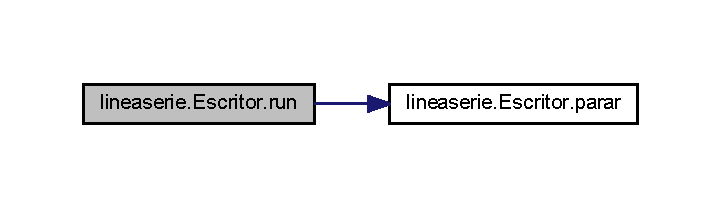
\includegraphics[width=346pt]{classlineaserie_1_1_escritor_a510a437d7f0ed6a89fb326b6d03e4d6c_cgraph}
\end{center}
\end{figure}


The documentation for this class was generated from the following file\+:\begin{DoxyCompactItemize}
\item 
C\+:/\+Users/jonmu/\+Desktop/\+P\+O\+P\+B\+L 4/src/lineaserie/\mbox{\hyperlink{_escritor_8java}{Escritor.\+java}}\end{DoxyCompactItemize}

\hypertarget{classimagenes_1_1_imagenes}{}\section{imagenes.\+Imagenes Class Reference}
\label{classimagenes_1_1_imagenes}\index{imagenes.\+Imagenes@{imagenes.\+Imagenes}}


Collaboration diagram for imagenes.\+Imagenes\+:\nopagebreak
\begin{figure}[H]
\begin{center}
\leavevmode
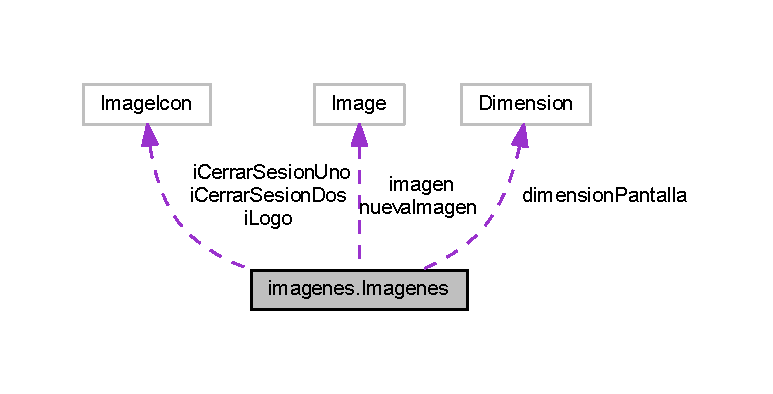
\includegraphics[width=350pt]{classimagenes_1_1_imagenes__coll__graph}
\end{center}
\end{figure}
\subsection*{Public Member Functions}
\begin{DoxyCompactItemize}
\item 
\mbox{\hyperlink{classimagenes_1_1_imagenes_a5306d3993cd1796bb3e7a027a5f2090c}{Imagenes}} ()  throws I\+O\+Exception 
\item 
Image\+Icon \mbox{\hyperlink{classimagenes_1_1_imagenes_a0f0caa5031d91592dd10a958b6b3bca0}{geti\+Dome}} ()
\item 
Image\+Icon \mbox{\hyperlink{classimagenes_1_1_imagenes_a35ea6dc13b089bcc087f73b5f5779219}{geti\+Cerrar\+Sesion\+Uno}} ()
\item 
Image\+Icon \mbox{\hyperlink{classimagenes_1_1_imagenes_a6ba10d5d816cbdf459d769b884940967}{geti\+Cerrar\+Sesion\+Dos}} ()
\end{DoxyCompactItemize}


\subsection{Detailed Description}


Definition at line 12 of file Imagenes.\+java.



\subsection{Constructor \& Destructor Documentation}
\mbox{\Hypertarget{classimagenes_1_1_imagenes_a5306d3993cd1796bb3e7a027a5f2090c}\label{classimagenes_1_1_imagenes_a5306d3993cd1796bb3e7a027a5f2090c}} 
\index{imagenes\+::\+Imagenes@{imagenes\+::\+Imagenes}!Imagenes@{Imagenes}}
\index{Imagenes@{Imagenes}!imagenes\+::\+Imagenes@{imagenes\+::\+Imagenes}}
\subsubsection{\texorpdfstring{Imagenes()}{Imagenes()}}
{\footnotesize\ttfamily imagenes.\+Imagenes.\+Imagenes (\begin{DoxyParamCaption}{ }\end{DoxyParamCaption}) throws I\+O\+Exception}



Definition at line 20 of file Imagenes.\+java.



\subsection{Member Function Documentation}
\mbox{\Hypertarget{classimagenes_1_1_imagenes_a6ba10d5d816cbdf459d769b884940967}\label{classimagenes_1_1_imagenes_a6ba10d5d816cbdf459d769b884940967}} 
\index{imagenes\+::\+Imagenes@{imagenes\+::\+Imagenes}!geti\+Cerrar\+Sesion\+Dos@{geti\+Cerrar\+Sesion\+Dos}}
\index{geti\+Cerrar\+Sesion\+Dos@{geti\+Cerrar\+Sesion\+Dos}!imagenes\+::\+Imagenes@{imagenes\+::\+Imagenes}}
\subsubsection{\texorpdfstring{geti\+Cerrar\+Sesion\+Dos()}{getiCerrarSesionDos()}}
{\footnotesize\ttfamily Image\+Icon imagenes.\+Imagenes.\+geti\+Cerrar\+Sesion\+Dos (\begin{DoxyParamCaption}{ }\end{DoxyParamCaption})}



Definition at line 54 of file Imagenes.\+java.

\mbox{\Hypertarget{classimagenes_1_1_imagenes_a35ea6dc13b089bcc087f73b5f5779219}\label{classimagenes_1_1_imagenes_a35ea6dc13b089bcc087f73b5f5779219}} 
\index{imagenes\+::\+Imagenes@{imagenes\+::\+Imagenes}!geti\+Cerrar\+Sesion\+Uno@{geti\+Cerrar\+Sesion\+Uno}}
\index{geti\+Cerrar\+Sesion\+Uno@{geti\+Cerrar\+Sesion\+Uno}!imagenes\+::\+Imagenes@{imagenes\+::\+Imagenes}}
\subsubsection{\texorpdfstring{geti\+Cerrar\+Sesion\+Uno()}{getiCerrarSesionUno()}}
{\footnotesize\ttfamily Image\+Icon imagenes.\+Imagenes.\+geti\+Cerrar\+Sesion\+Uno (\begin{DoxyParamCaption}{ }\end{DoxyParamCaption})}



Definition at line 49 of file Imagenes.\+java.

\mbox{\Hypertarget{classimagenes_1_1_imagenes_a0f0caa5031d91592dd10a958b6b3bca0}\label{classimagenes_1_1_imagenes_a0f0caa5031d91592dd10a958b6b3bca0}} 
\index{imagenes\+::\+Imagenes@{imagenes\+::\+Imagenes}!geti\+Dome@{geti\+Dome}}
\index{geti\+Dome@{geti\+Dome}!imagenes\+::\+Imagenes@{imagenes\+::\+Imagenes}}
\subsubsection{\texorpdfstring{geti\+Dome()}{getiDome()}}
{\footnotesize\ttfamily Image\+Icon imagenes.\+Imagenes.\+geti\+Dome (\begin{DoxyParamCaption}{ }\end{DoxyParamCaption})}



Definition at line 44 of file Imagenes.\+java.



The documentation for this class was generated from the following file\+:\begin{DoxyCompactItemize}
\item 
C\+:/\+Users/jonmu/\+Desktop/\+P\+O\+P\+B\+L 4/src/imagenes/\mbox{\hyperlink{_imagenes_8java}{Imagenes.\+java}}\end{DoxyCompactItemize}

\hypertarget{classlineaserie_1_1_inicializador}{}\section{lineaserie.\+Inicializador Class Reference}
\label{classlineaserie_1_1_inicializador}\index{lineaserie.\+Inicializador@{lineaserie.\+Inicializador}}


Inheritance diagram for lineaserie.\+Inicializador\+:
% FIG 0


Collaboration diagram for lineaserie.\+Inicializador\+:
% FIG 1
\subsection*{Public Member Functions}
\begin{DoxyCompactItemize}
\item 
\mbox{\Hypertarget{classlineaserie_1_1_inicializador_a86958a2a419199116654e4f259e86a66}\label{classlineaserie_1_1_inicializador_a86958a2a419199116654e4f259e86a66}} 
{\bfseries Inicializador} (\mbox{\hyperlink{classvistas_1_1_principal}{Principal}} principal)
\item 
\mbox{\Hypertarget{classlineaserie_1_1_inicializador_a8163b9059ff9417835aae96eddd8464a}\label{classlineaserie_1_1_inicializador_a8163b9059ff9417835aae96eddd8464a}} 
void {\bfseries run} ()
\end{DoxyCompactItemize}


The documentation for this class was generated from the following file\+:\begin{DoxyCompactItemize}
\item 
C\+:/\+Users/jonmu/\+Desktop/\+P\+O\+P\+B\+L 4/src/lineaserie/Inicializador.\+java\end{DoxyCompactItemize}

\hypertarget{classlineaserie_1_1_lector}{}\section{lineaserie.\+Lector Class Reference}
\label{classlineaserie_1_1_lector}\index{lineaserie.\+Lector@{lineaserie.\+Lector}}


Inheritance diagram for lineaserie.\+Lector\+:
\nopagebreak
\begin{figure}[H]
\begin{center}
\leavevmode
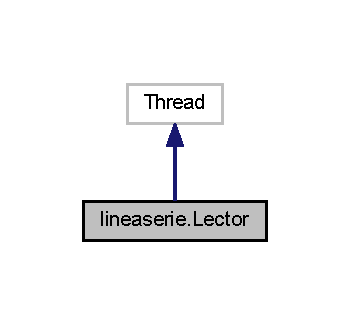
\includegraphics[width=168pt]{classlineaserie_1_1_lector__inherit__graph}
\end{center}
\end{figure}


Collaboration diagram for lineaserie.\+Lector\+:
\nopagebreak
\begin{figure}[H]
\begin{center}
\leavevmode
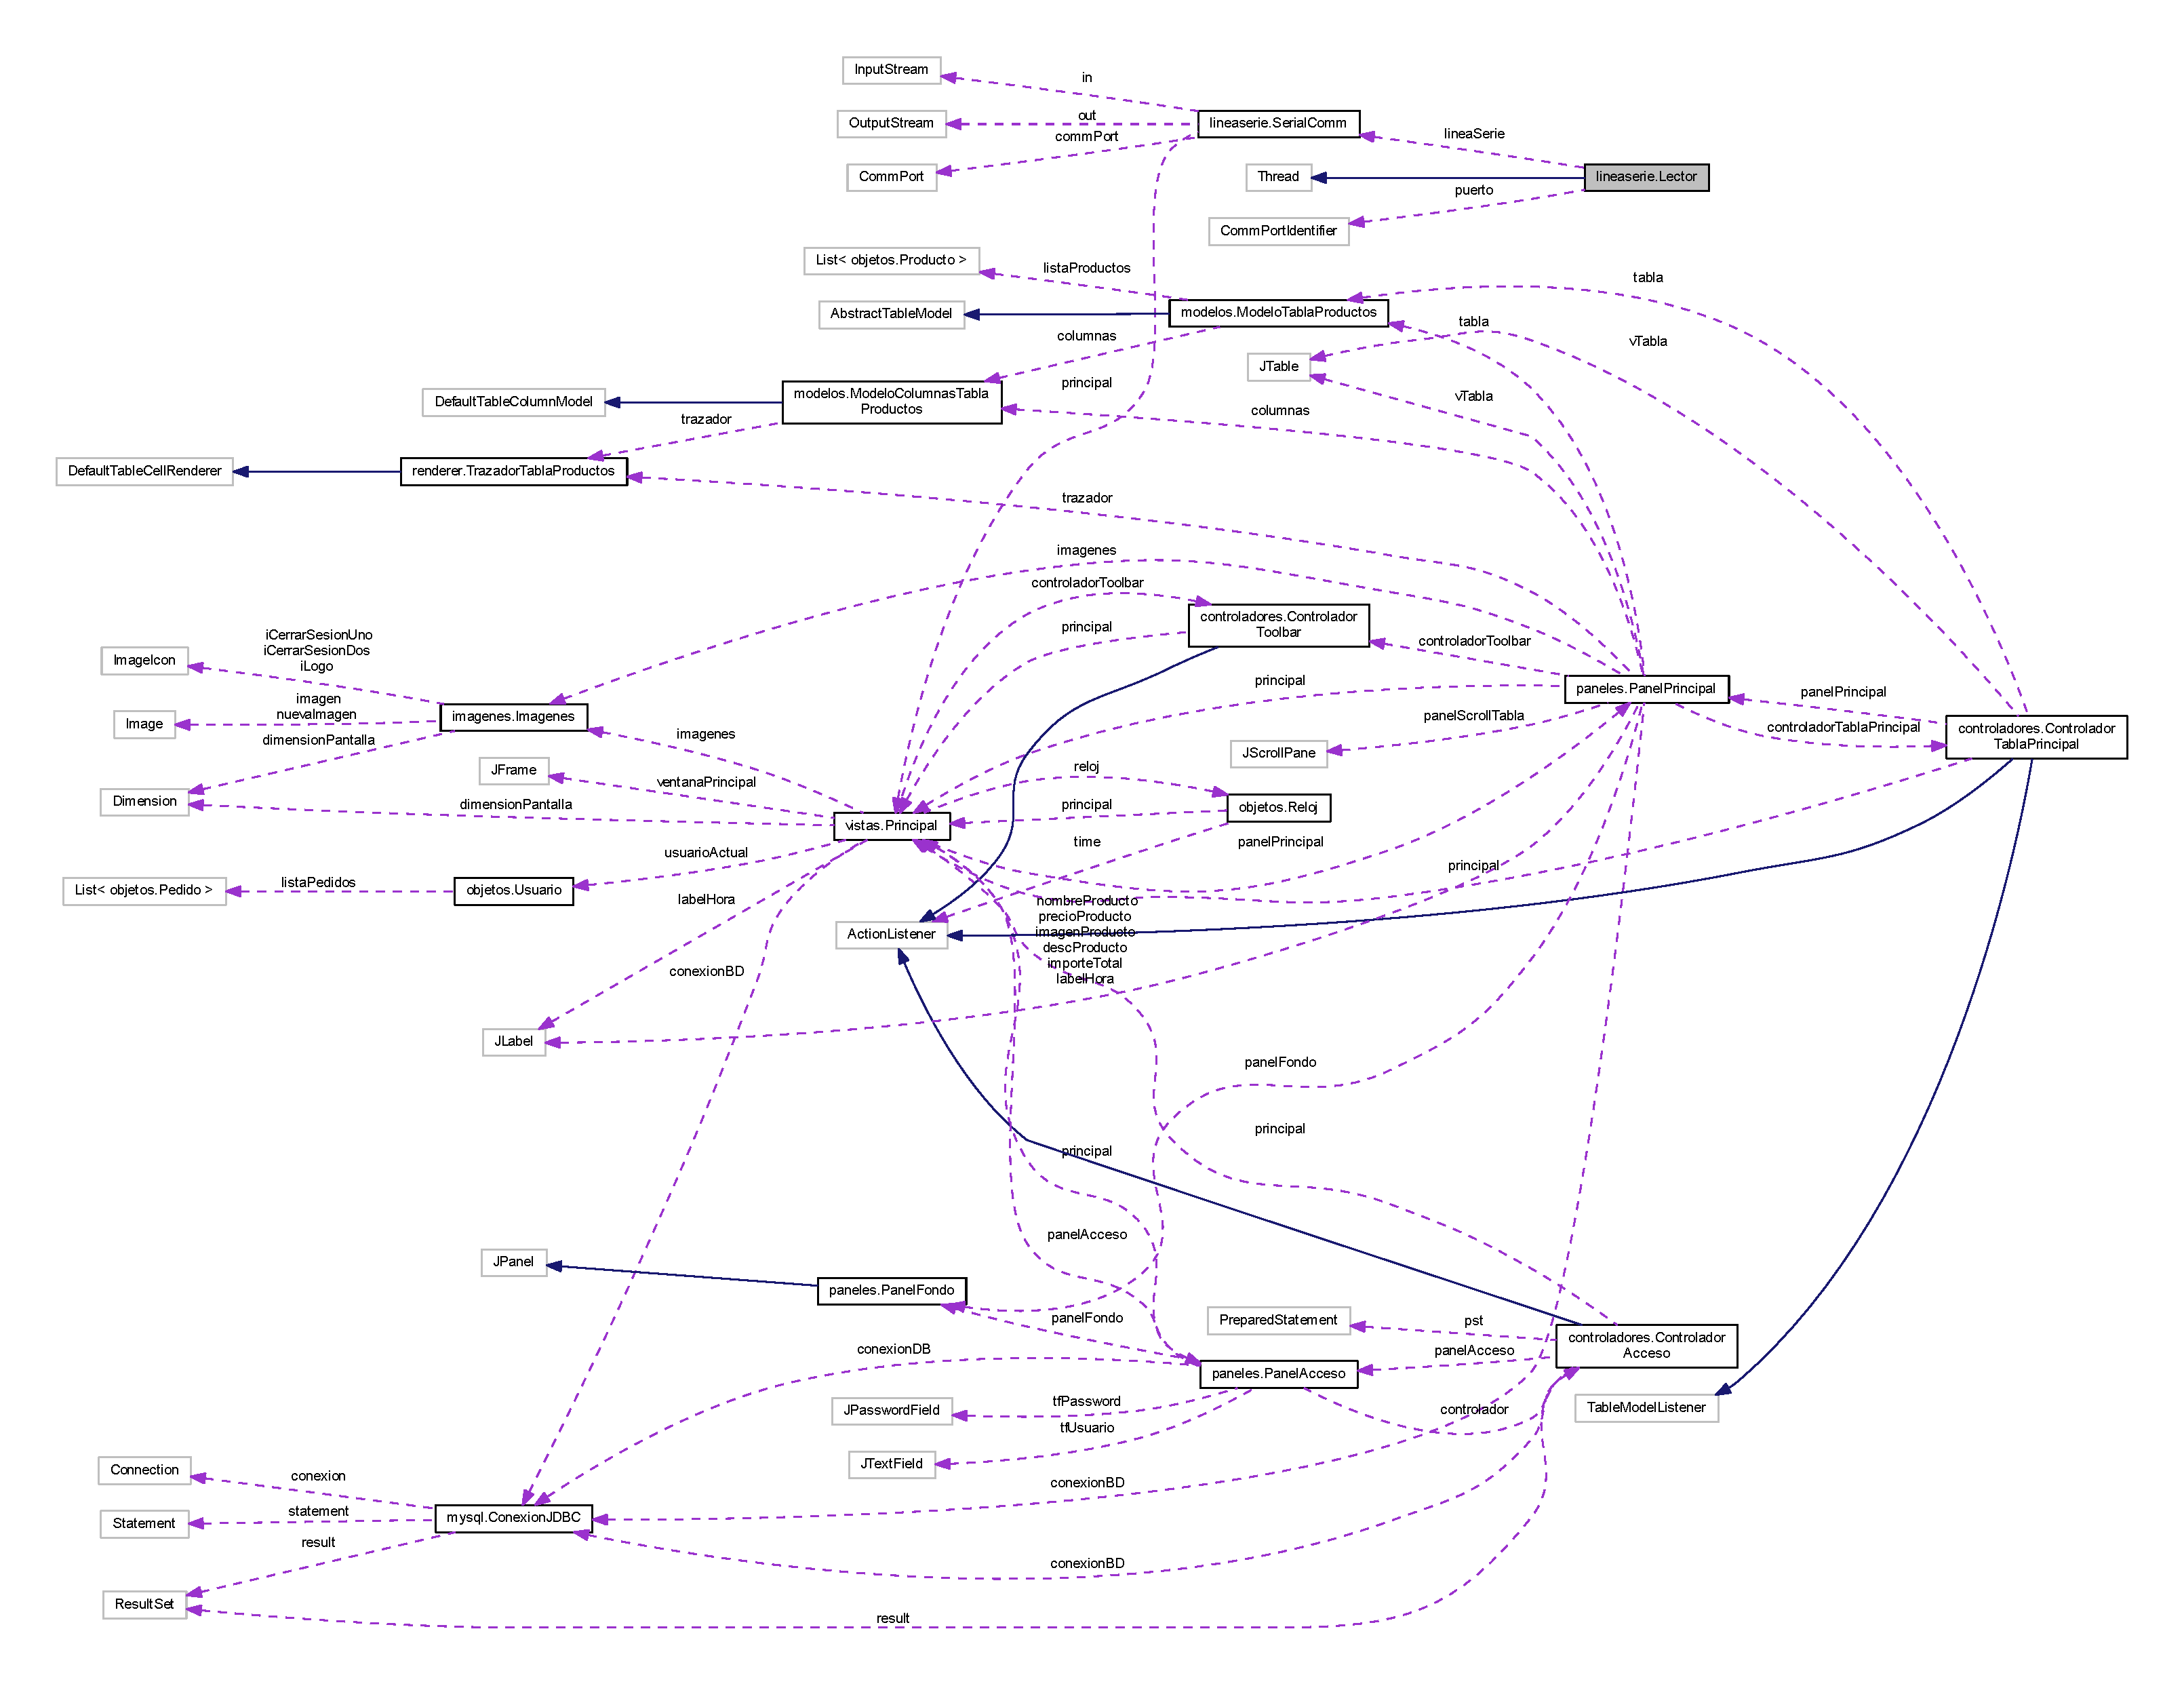
\includegraphics[width=350pt]{classlineaserie_1_1_lector__coll__graph}
\end{center}
\end{figure}
\subsection*{Public Member Functions}
\begin{DoxyCompactItemize}
\item 
\mbox{\hyperlink{classlineaserie_1_1_lector_a49947c6538f2b7e0b423b7664c252ed3}{Lector}} (\mbox{\hyperlink{classlineaserie_1_1_serial_comm}{Serial\+Comm}} linea\+Serie, Comm\+Port\+Identifier puerto)
\item 
void \mbox{\hyperlink{classlineaserie_1_1_lector_ac57211de70ab9a4bd7aa80ab491f7fca}{run}} ()
\item 
void \mbox{\hyperlink{classlineaserie_1_1_lector_a7abfb09ecc456931b8948a058cedf4c8}{parar}} ()
\end{DoxyCompactItemize}


\subsection{Detailed Description}


Definition at line 9 of file Lector.\+java.



\subsection{Constructor \& Destructor Documentation}
\mbox{\Hypertarget{classlineaserie_1_1_lector_a49947c6538f2b7e0b423b7664c252ed3}\label{classlineaserie_1_1_lector_a49947c6538f2b7e0b423b7664c252ed3}} 
\index{lineaserie\+::\+Lector@{lineaserie\+::\+Lector}!Lector@{Lector}}
\index{Lector@{Lector}!lineaserie\+::\+Lector@{lineaserie\+::\+Lector}}
\subsubsection{\texorpdfstring{Lector()}{Lector()}}
{\footnotesize\ttfamily lineaserie.\+Lector.\+Lector (\begin{DoxyParamCaption}\item[{\mbox{\hyperlink{classlineaserie_1_1_serial_comm}{Serial\+Comm}}}]{linea\+Serie,  }\item[{Comm\+Port\+Identifier}]{puerto }\end{DoxyParamCaption})}



Definition at line 15 of file Lector.\+java.



\subsection{Member Function Documentation}
\mbox{\Hypertarget{classlineaserie_1_1_lector_a7abfb09ecc456931b8948a058cedf4c8}\label{classlineaserie_1_1_lector_a7abfb09ecc456931b8948a058cedf4c8}} 
\index{lineaserie\+::\+Lector@{lineaserie\+::\+Lector}!parar@{parar}}
\index{parar@{parar}!lineaserie\+::\+Lector@{lineaserie\+::\+Lector}}
\subsubsection{\texorpdfstring{parar()}{parar()}}
{\footnotesize\ttfamily void lineaserie.\+Lector.\+parar (\begin{DoxyParamCaption}{ }\end{DoxyParamCaption})}



Definition at line 32 of file Lector.\+java.

\mbox{\Hypertarget{classlineaserie_1_1_lector_ac57211de70ab9a4bd7aa80ab491f7fca}\label{classlineaserie_1_1_lector_ac57211de70ab9a4bd7aa80ab491f7fca}} 
\index{lineaserie\+::\+Lector@{lineaserie\+::\+Lector}!run@{run}}
\index{run@{run}!lineaserie\+::\+Lector@{lineaserie\+::\+Lector}}
\subsubsection{\texorpdfstring{run()}{run()}}
{\footnotesize\ttfamily void lineaserie.\+Lector.\+run (\begin{DoxyParamCaption}{ }\end{DoxyParamCaption})}



Definition at line 22 of file Lector.\+java.

Here is the call graph for this function\+:
\nopagebreak
\begin{figure}[H]
\begin{center}
\leavevmode
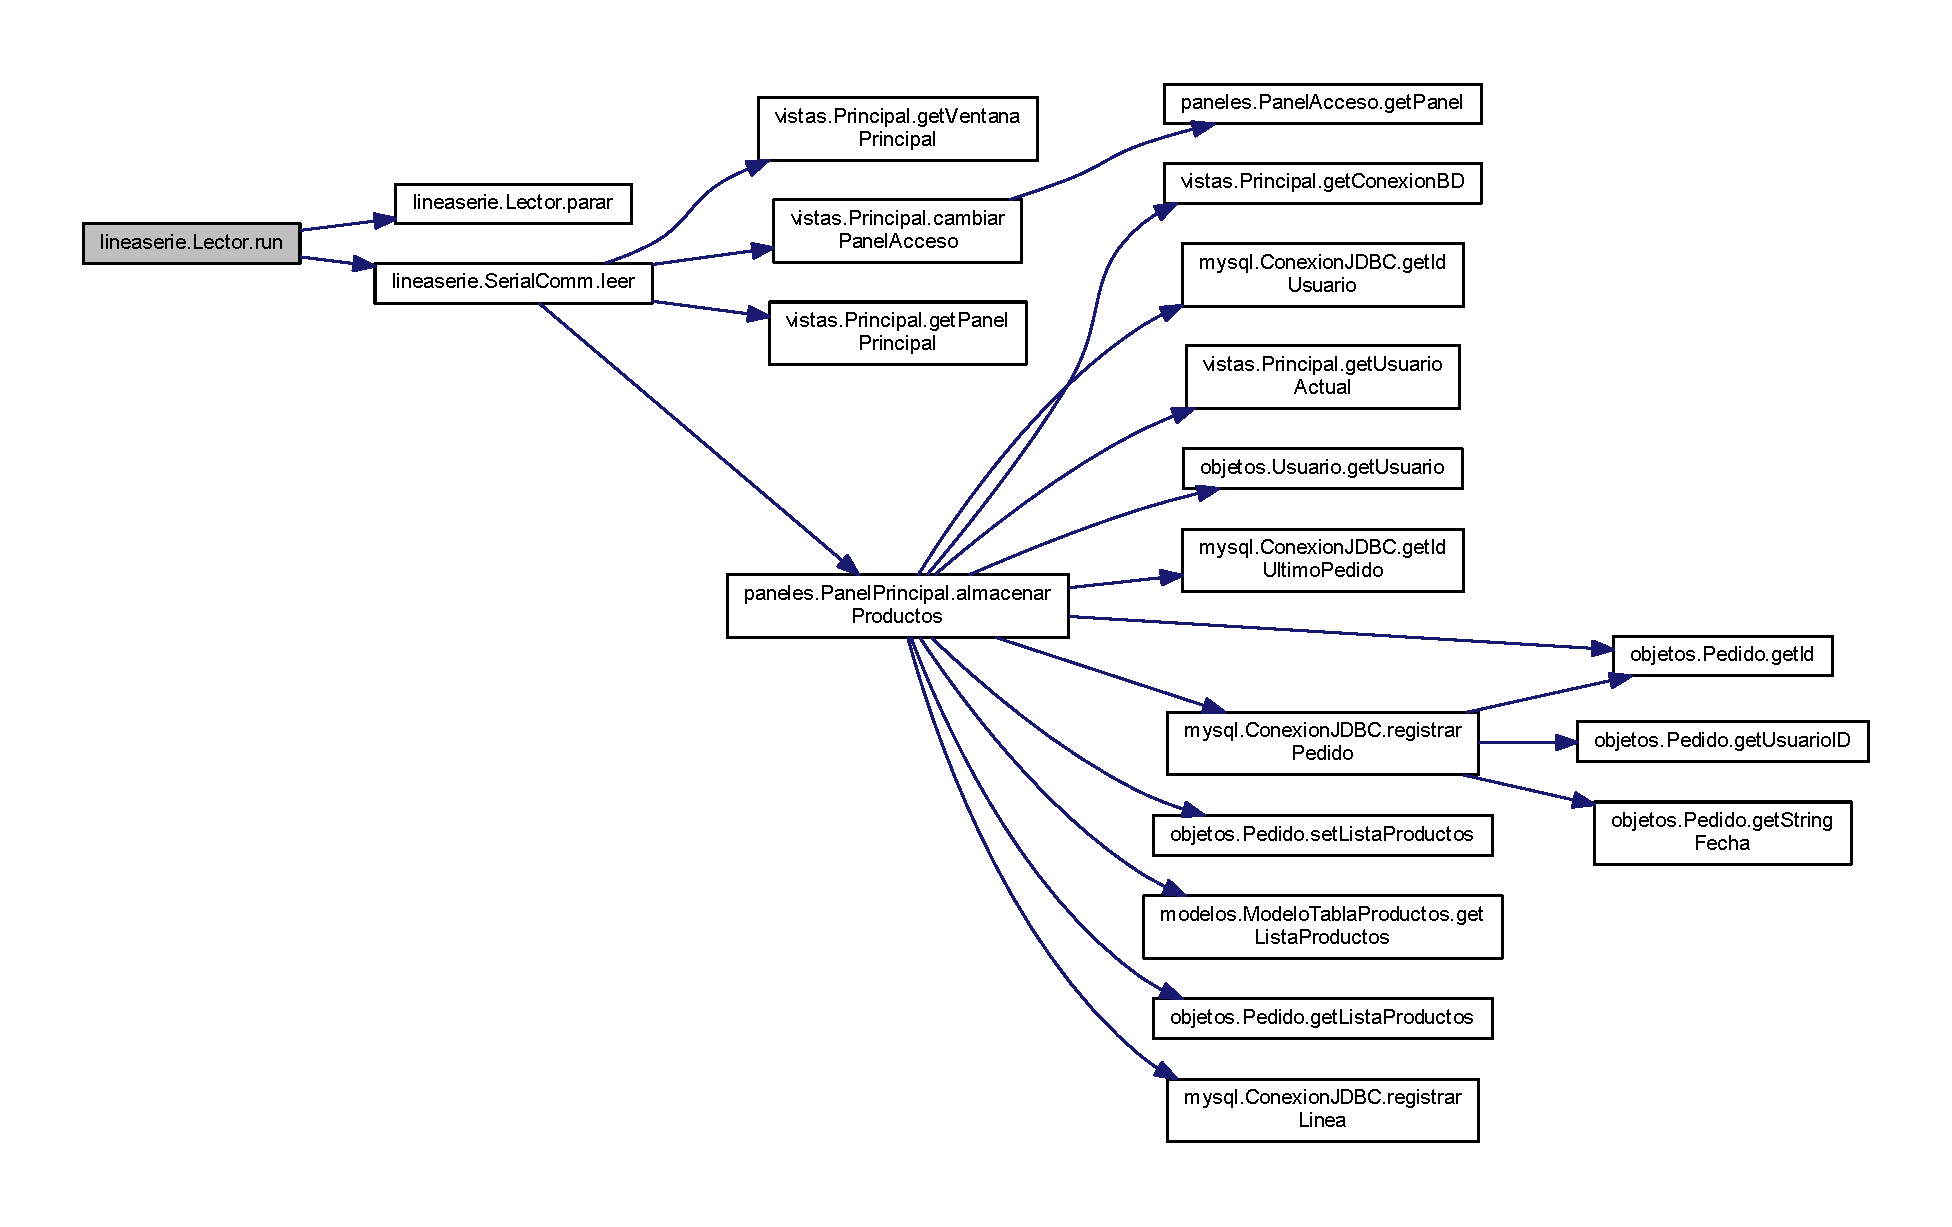
\includegraphics[width=350pt]{classlineaserie_1_1_lector_ac57211de70ab9a4bd7aa80ab491f7fca_cgraph}
\end{center}
\end{figure}


The documentation for this class was generated from the following file\+:\begin{DoxyCompactItemize}
\item 
C\+:/\+Users/jonmu/\+Desktop/\+P\+O\+P\+B\+L 4/src/lineaserie/\mbox{\hyperlink{_lector_8java}{Lector.\+java}}\end{DoxyCompactItemize}

\hypertarget{classobjetos_1_1_maquina}{}\section{objetos.\+Maquina Class Reference}
\label{classobjetos_1_1_maquina}\index{objetos.\+Maquina@{objetos.\+Maquina}}
\subsection*{Public Member Functions}
\begin{DoxyCompactItemize}
\item 
\mbox{\Hypertarget{classobjetos_1_1_maquina_abe32f06ca4367bea60d592d504a7a359}\label{classobjetos_1_1_maquina_abe32f06ca4367bea60d592d504a7a359}} 
{\bfseries Maquina} (boolean estado, int id)
\item 
\mbox{\Hypertarget{classobjetos_1_1_maquina_a03b4c97926e8db81a5a28459293c16b6}\label{classobjetos_1_1_maquina_a03b4c97926e8db81a5a28459293c16b6}} 
boolean {\bfseries is\+Estado} ()
\item 
\mbox{\Hypertarget{classobjetos_1_1_maquina_a8a5d703c85d9a8a4a7ff352b01ff085b}\label{classobjetos_1_1_maquina_a8a5d703c85d9a8a4a7ff352b01ff085b}} 
void {\bfseries set\+Estado} (boolean estado)
\item 
\mbox{\Hypertarget{classobjetos_1_1_maquina_aca30cab810f1072e9ab07024d6f97cc6}\label{classobjetos_1_1_maquina_aca30cab810f1072e9ab07024d6f97cc6}} 
int {\bfseries get\+Id} ()
\item 
\mbox{\Hypertarget{classobjetos_1_1_maquina_a8ecfb51ac52f34402a48c572aa710297}\label{classobjetos_1_1_maquina_a8ecfb51ac52f34402a48c572aa710297}} 
Class$<$?$>$ {\bfseries get\+Field\+Class} (int indice)
\item 
\mbox{\Hypertarget{classobjetos_1_1_maquina_ab50c4dec88d2de79313a9a369df0ffd3}\label{classobjetos_1_1_maquina_ab50c4dec88d2de79313a9a369df0ffd3}} 
Object {\bfseries get\+Field\+At} (int columna)
\end{DoxyCompactItemize}


The documentation for this class was generated from the following file\+:\begin{DoxyCompactItemize}
\item 
C\+:/\+Users/jonmu/\+Desktop/\+P\+O\+P\+B\+L 4/src/objetos/Maquina.\+java\end{DoxyCompactItemize}

\hypertarget{classmodelos_1_1_modelo_columnas_tabla}{}\section{modelos.\+Modelo\+Columnas\+Tabla Class Reference}
\label{classmodelos_1_1_modelo_columnas_tabla}\index{modelos.\+Modelo\+Columnas\+Tabla@{modelos.\+Modelo\+Columnas\+Tabla}}


Inheritance diagram for modelos.\+Modelo\+Columnas\+Tabla\+:
% FIG 0


Collaboration diagram for modelos.\+Modelo\+Columnas\+Tabla\+:
% FIG 1
\subsection*{Public Member Functions}
\begin{DoxyCompactItemize}
\item 
\mbox{\Hypertarget{classmodelos_1_1_modelo_columnas_tabla_a1ac636f1d60b6abb63e86834e6c8f09d}\label{classmodelos_1_1_modelo_columnas_tabla_a1ac636f1d60b6abb63e86834e6c8f09d}} 
{\bfseries Modelo\+Columnas\+Tabla} (\mbox{\hyperlink{classmodelos_1_1_trazador_tabla_maquina}{Trazador\+Tabla\+Maquina}} trazador)
\end{DoxyCompactItemize}


The documentation for this class was generated from the following file\+:\begin{DoxyCompactItemize}
\item 
C\+:/\+Users/jonmu/\+Desktop/\+P\+O\+P\+B\+L 4/src/modelos/Modelo\+Columnas\+Tabla.\+java\end{DoxyCompactItemize}

\hypertarget{classmodelos_1_1_modelo_columnas_tabla_productos}{}\section{modelos.\+Modelo\+Columnas\+Tabla\+Productos Class Reference}
\label{classmodelos_1_1_modelo_columnas_tabla_productos}\index{modelos.\+Modelo\+Columnas\+Tabla\+Productos@{modelos.\+Modelo\+Columnas\+Tabla\+Productos}}


Inheritance diagram for modelos.\+Modelo\+Columnas\+Tabla\+Productos\+:
% FIG 0


Collaboration diagram for modelos.\+Modelo\+Columnas\+Tabla\+Productos\+:
% FIG 1
\subsection*{Public Member Functions}
\begin{DoxyCompactItemize}
\item 
\mbox{\Hypertarget{classmodelos_1_1_modelo_columnas_tabla_productos_a7807b42a8c5c5630006122c92b2d9a84}\label{classmodelos_1_1_modelo_columnas_tabla_productos_a7807b42a8c5c5630006122c92b2d9a84}} 
{\bfseries Modelo\+Columnas\+Tabla\+Productos} (\mbox{\hyperlink{classrenderer_1_1_trazador_tabla_productos}{Trazador\+Tabla\+Productos}} trazador)
\end{DoxyCompactItemize}


The documentation for this class was generated from the following file\+:\begin{DoxyCompactItemize}
\item 
C\+:/\+Users/jonmu/\+Desktop/\+P\+O\+P\+B\+L 4/src/modelos/Modelo\+Columnas\+Tabla\+Productos.\+java\end{DoxyCompactItemize}

\hypertarget{classmodelos_1_1_modelo_pedidos}{}\section{modelos.\+Modelo\+Pedidos Class Reference}
\label{classmodelos_1_1_modelo_pedidos}\index{modelos.\+Modelo\+Pedidos@{modelos.\+Modelo\+Pedidos}}


Inheritance diagram for modelos.\+Modelo\+Pedidos\+:
% FIG 0


Collaboration diagram for modelos.\+Modelo\+Pedidos\+:
% FIG 1
\subsection*{Public Member Functions}
\begin{DoxyCompactItemize}
\item 
\mbox{\Hypertarget{classmodelos_1_1_modelo_pedidos_aa994e01ae994d8e3bf55be7272602fb3}\label{classmodelos_1_1_modelo_pedidos_aa994e01ae994d8e3bf55be7272602fb3}} 
void {\bfseries set\+Lista\+Pedidos} (\mbox{\hyperlink{classobjetos_1_1_usuario}{Usuario}} u)
\item 
\mbox{\Hypertarget{classmodelos_1_1_modelo_pedidos_a6e263f0ee1c3e06067671cad86e8530f}\label{classmodelos_1_1_modelo_pedidos_a6e263f0ee1c3e06067671cad86e8530f}} 
int {\bfseries get\+Size} ()
\item 
\mbox{\Hypertarget{classmodelos_1_1_modelo_pedidos_a1b9a1858545410c5447e9ec1a2c46c20}\label{classmodelos_1_1_modelo_pedidos_a1b9a1858545410c5447e9ec1a2c46c20}} 
\mbox{\hyperlink{classobjetos_1_1_pedido}{Pedido}} {\bfseries get\+Element\+At} (int index)
\item 
\mbox{\Hypertarget{classmodelos_1_1_modelo_pedidos_a6493faaa5807821e134db0a62bc93425}\label{classmodelos_1_1_modelo_pedidos_a6493faaa5807821e134db0a62bc93425}} 
void {\bfseries limpiar} ()
\item 
\mbox{\Hypertarget{classmodelos_1_1_modelo_pedidos_a6a817c290edad02cffcb390716ec3f45}\label{classmodelos_1_1_modelo_pedidos_a6a817c290edad02cffcb390716ec3f45}} 
void {\bfseries mostrar\+Todos} ()
\item 
\mbox{\Hypertarget{classmodelos_1_1_modelo_pedidos_ac040d81e35f1db869c8d0664bf6b0b60}\label{classmodelos_1_1_modelo_pedidos_ac040d81e35f1db869c8d0664bf6b0b60}} 
void {\bfseries filtrar\+Por\+A�o} (String filtro)
\item 
\mbox{\Hypertarget{classmodelos_1_1_modelo_pedidos_a404af1e93f8946cb06aa531e8043c62c}\label{classmodelos_1_1_modelo_pedidos_a404af1e93f8946cb06aa531e8043c62c}} 
void {\bfseries filtrar\+Por\+Mes} (String filtro)
\item 
\mbox{\Hypertarget{classmodelos_1_1_modelo_pedidos_ae7e731e868e782dcc6296250e759b436}\label{classmodelos_1_1_modelo_pedidos_ae7e731e868e782dcc6296250e759b436}} 
void {\bfseries filtrar\+Por\+Mes\+Y\+A�o} (String filtro1, String filtro2)
\end{DoxyCompactItemize}


The documentation for this class was generated from the following file\+:\begin{DoxyCompactItemize}
\item 
C\+:/\+Users/jonmu/\+Desktop/\+P\+O\+P\+B\+L 4/src/modelos/Modelo\+Pedidos.\+java\end{DoxyCompactItemize}

\hypertarget{classmodelos_1_1_modelo_tabla_maquina}{}\section{modelos.\+Modelo\+Tabla\+Maquina Class Reference}
\label{classmodelos_1_1_modelo_tabla_maquina}\index{modelos.\+Modelo\+Tabla\+Maquina@{modelos.\+Modelo\+Tabla\+Maquina}}


Inheritance diagram for modelos.\+Modelo\+Tabla\+Maquina\+:
\nopagebreak
\begin{figure}[H]
\begin{center}
\leavevmode
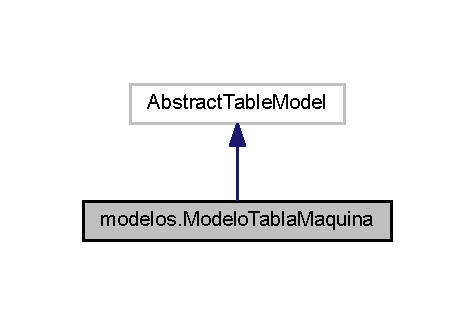
\includegraphics[width=228pt]{classmodelos_1_1_modelo_tabla_maquina__inherit__graph}
\end{center}
\end{figure}


Collaboration diagram for modelos.\+Modelo\+Tabla\+Maquina\+:
\nopagebreak
\begin{figure}[H]
\begin{center}
\leavevmode
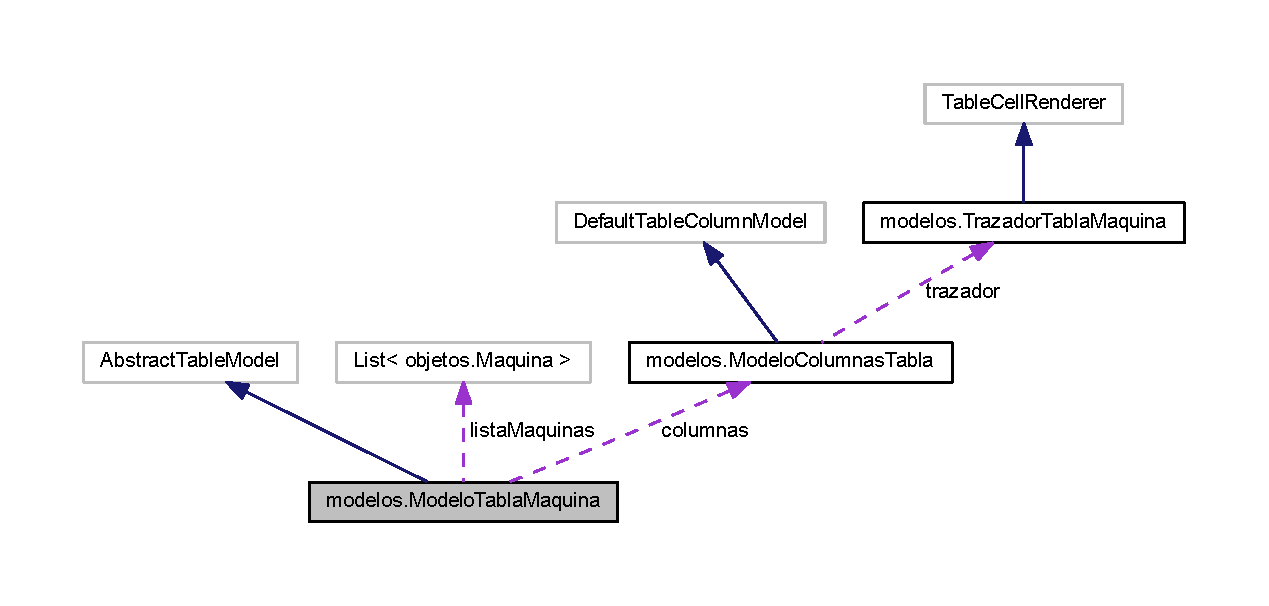
\includegraphics[width=350pt]{classmodelos_1_1_modelo_tabla_maquina__coll__graph}
\end{center}
\end{figure}
\subsection*{Public Member Functions}
\begin{DoxyCompactItemize}
\item 
\mbox{\hyperlink{classmodelos_1_1_modelo_tabla_maquina_a1a20d87af57c2ec9a090f9f164f616cc}{Modelo\+Tabla\+Maquina}} (\mbox{\hyperlink{classmodelos_1_1_modelo_columnas_tabla}{Modelo\+Columnas\+Tabla}} columnas, List$<$ \mbox{\hyperlink{classobjetos_1_1_maquina}{Maquina}} $>$ lista)
\item 
void \mbox{\hyperlink{classmodelos_1_1_modelo_tabla_maquina_aac1f2793dfa5765b8e66c17891753e10}{delete}} (int index)
\item 
void \mbox{\hyperlink{classmodelos_1_1_modelo_tabla_maquina_aa49c15eda1d441b2a17159f0aa80cef4}{add}} (\mbox{\hyperlink{classobjetos_1_1_maquina}{Maquina}} e)
\item 
List$<$ \mbox{\hyperlink{classobjetos_1_1_maquina}{Maquina}} $>$ \mbox{\hyperlink{classmodelos_1_1_modelo_tabla_maquina_a557771e167f337141e22d3d4a0432b7b}{getlista\+Maquinas}} ()
\item 
void \mbox{\hyperlink{classmodelos_1_1_modelo_tabla_maquina_a559a21bd653aa7b639fa598ff22fa5f7}{setlista\+Maquinas}} (List$<$ \mbox{\hyperlink{classobjetos_1_1_maquina}{Maquina}} $>$ lista\+Maquinas)
\item 
void \mbox{\hyperlink{classmodelos_1_1_modelo_tabla_maquina_ab8ce1d5c3842d65c11a8c8cb10f5b7f7}{cambiar\+Estado}} (int indice)
\item 
void \mbox{\hyperlink{classmodelos_1_1_modelo_tabla_maquina_a48d1751bbb3bfb91d50eb5bd2a80207e}{refrescar\+Tabla}} ()
\item 
int \mbox{\hyperlink{classmodelos_1_1_modelo_tabla_maquina_aa380cce066ff74a0a7f95ae4d9388eb9}{get\+Row\+Count}} ()
\item 
Boolean \mbox{\hyperlink{classmodelos_1_1_modelo_tabla_maquina_a76d930fbec2a211e91095ac641f030cb}{get\+Value\+At2}} (int fila, int columna)
\item 
Object \mbox{\hyperlink{classmodelos_1_1_modelo_tabla_maquina_ae6611198ecf631949ddb041b8231da95}{get\+Value\+At}} (int fila, int columna)
\item 
boolean \mbox{\hyperlink{classmodelos_1_1_modelo_tabla_maquina_ab81f2b02aa2cc4c0f9c93111ba345df8}{is\+Cell\+Editable}} (int row\+Index, int column\+Index)
\item 
Class$<$?$>$ \mbox{\hyperlink{classmodelos_1_1_modelo_tabla_maquina_a29f3df9756e2a5e9a66bde094a1ee56e}{get\+Column\+Class}} (int column\+Index)
\item 
int \mbox{\hyperlink{classmodelos_1_1_modelo_tabla_maquina_a83f4d721197d932523e11de1155cbad6}{get\+Column\+Count}} ()
\end{DoxyCompactItemize}


\subsection{Detailed Description}


Definition at line 9 of file Modelo\+Tabla\+Maquina.\+java.



\subsection{Constructor \& Destructor Documentation}
\mbox{\Hypertarget{classmodelos_1_1_modelo_tabla_maquina_a1a20d87af57c2ec9a090f9f164f616cc}\label{classmodelos_1_1_modelo_tabla_maquina_a1a20d87af57c2ec9a090f9f164f616cc}} 
\index{modelos\+::\+Modelo\+Tabla\+Maquina@{modelos\+::\+Modelo\+Tabla\+Maquina}!Modelo\+Tabla\+Maquina@{Modelo\+Tabla\+Maquina}}
\index{Modelo\+Tabla\+Maquina@{Modelo\+Tabla\+Maquina}!modelos\+::\+Modelo\+Tabla\+Maquina@{modelos\+::\+Modelo\+Tabla\+Maquina}}
\subsubsection{\texorpdfstring{Modelo\+Tabla\+Maquina()}{ModeloTablaMaquina()}}
{\footnotesize\ttfamily modelos.\+Modelo\+Tabla\+Maquina.\+Modelo\+Tabla\+Maquina (\begin{DoxyParamCaption}\item[{\mbox{\hyperlink{classmodelos_1_1_modelo_columnas_tabla}{Modelo\+Columnas\+Tabla}}}]{columnas,  }\item[{List$<$ \mbox{\hyperlink{classobjetos_1_1_maquina}{Maquina}} $>$}]{lista }\end{DoxyParamCaption})}



Definition at line 18 of file Modelo\+Tabla\+Maquina.\+java.



\subsection{Member Function Documentation}
\mbox{\Hypertarget{classmodelos_1_1_modelo_tabla_maquina_aa49c15eda1d441b2a17159f0aa80cef4}\label{classmodelos_1_1_modelo_tabla_maquina_aa49c15eda1d441b2a17159f0aa80cef4}} 
\index{modelos\+::\+Modelo\+Tabla\+Maquina@{modelos\+::\+Modelo\+Tabla\+Maquina}!add@{add}}
\index{add@{add}!modelos\+::\+Modelo\+Tabla\+Maquina@{modelos\+::\+Modelo\+Tabla\+Maquina}}
\subsubsection{\texorpdfstring{add()}{add()}}
{\footnotesize\ttfamily void modelos.\+Modelo\+Tabla\+Maquina.\+add (\begin{DoxyParamCaption}\item[{\mbox{\hyperlink{classobjetos_1_1_maquina}{Maquina}}}]{e }\end{DoxyParamCaption})}



Definition at line 30 of file Modelo\+Tabla\+Maquina.\+java.

\mbox{\Hypertarget{classmodelos_1_1_modelo_tabla_maquina_ab8ce1d5c3842d65c11a8c8cb10f5b7f7}\label{classmodelos_1_1_modelo_tabla_maquina_ab8ce1d5c3842d65c11a8c8cb10f5b7f7}} 
\index{modelos\+::\+Modelo\+Tabla\+Maquina@{modelos\+::\+Modelo\+Tabla\+Maquina}!cambiar\+Estado@{cambiar\+Estado}}
\index{cambiar\+Estado@{cambiar\+Estado}!modelos\+::\+Modelo\+Tabla\+Maquina@{modelos\+::\+Modelo\+Tabla\+Maquina}}
\subsubsection{\texorpdfstring{cambiar\+Estado()}{cambiarEstado()}}
{\footnotesize\ttfamily void modelos.\+Modelo\+Tabla\+Maquina.\+cambiar\+Estado (\begin{DoxyParamCaption}\item[{int}]{indice }\end{DoxyParamCaption})}



Definition at line 43 of file Modelo\+Tabla\+Maquina.\+java.

\mbox{\Hypertarget{classmodelos_1_1_modelo_tabla_maquina_aac1f2793dfa5765b8e66c17891753e10}\label{classmodelos_1_1_modelo_tabla_maquina_aac1f2793dfa5765b8e66c17891753e10}} 
\index{modelos\+::\+Modelo\+Tabla\+Maquina@{modelos\+::\+Modelo\+Tabla\+Maquina}!delete@{delete}}
\index{delete@{delete}!modelos\+::\+Modelo\+Tabla\+Maquina@{modelos\+::\+Modelo\+Tabla\+Maquina}}
\subsubsection{\texorpdfstring{delete()}{delete()}}
{\footnotesize\ttfamily void modelos.\+Modelo\+Tabla\+Maquina.\+delete (\begin{DoxyParamCaption}\item[{int}]{index }\end{DoxyParamCaption})}



Definition at line 25 of file Modelo\+Tabla\+Maquina.\+java.

\mbox{\Hypertarget{classmodelos_1_1_modelo_tabla_maquina_a29f3df9756e2a5e9a66bde094a1ee56e}\label{classmodelos_1_1_modelo_tabla_maquina_a29f3df9756e2a5e9a66bde094a1ee56e}} 
\index{modelos\+::\+Modelo\+Tabla\+Maquina@{modelos\+::\+Modelo\+Tabla\+Maquina}!get\+Column\+Class@{get\+Column\+Class}}
\index{get\+Column\+Class@{get\+Column\+Class}!modelos\+::\+Modelo\+Tabla\+Maquina@{modelos\+::\+Modelo\+Tabla\+Maquina}}
\subsubsection{\texorpdfstring{get\+Column\+Class()}{getColumnClass()}}
{\footnotesize\ttfamily Class$<$?$>$ modelos.\+Modelo\+Tabla\+Maquina.\+get\+Column\+Class (\begin{DoxyParamCaption}\item[{int}]{column\+Index }\end{DoxyParamCaption})}



Definition at line 84 of file Modelo\+Tabla\+Maquina.\+java.

Here is the call graph for this function\+:
\nopagebreak
\begin{figure}[H]
\begin{center}
\leavevmode
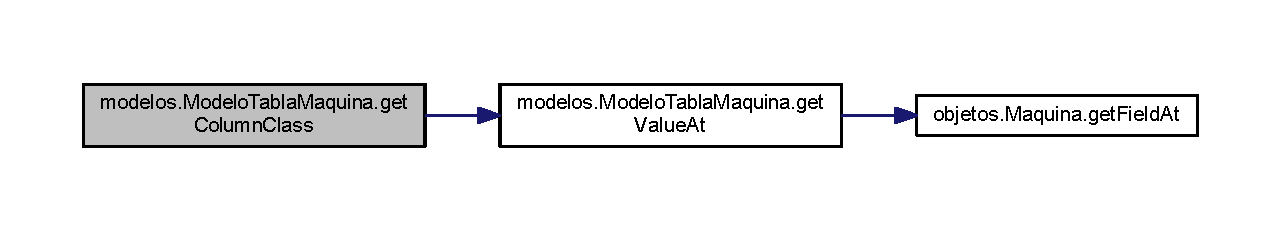
\includegraphics[width=350pt]{classmodelos_1_1_modelo_tabla_maquina_a29f3df9756e2a5e9a66bde094a1ee56e_cgraph}
\end{center}
\end{figure}
\mbox{\Hypertarget{classmodelos_1_1_modelo_tabla_maquina_a83f4d721197d932523e11de1155cbad6}\label{classmodelos_1_1_modelo_tabla_maquina_a83f4d721197d932523e11de1155cbad6}} 
\index{modelos\+::\+Modelo\+Tabla\+Maquina@{modelos\+::\+Modelo\+Tabla\+Maquina}!get\+Column\+Count@{get\+Column\+Count}}
\index{get\+Column\+Count@{get\+Column\+Count}!modelos\+::\+Modelo\+Tabla\+Maquina@{modelos\+::\+Modelo\+Tabla\+Maquina}}
\subsubsection{\texorpdfstring{get\+Column\+Count()}{getColumnCount()}}
{\footnotesize\ttfamily int modelos.\+Modelo\+Tabla\+Maquina.\+get\+Column\+Count (\begin{DoxyParamCaption}{ }\end{DoxyParamCaption})}



Definition at line 90 of file Modelo\+Tabla\+Maquina.\+java.

\mbox{\Hypertarget{classmodelos_1_1_modelo_tabla_maquina_a557771e167f337141e22d3d4a0432b7b}\label{classmodelos_1_1_modelo_tabla_maquina_a557771e167f337141e22d3d4a0432b7b}} 
\index{modelos\+::\+Modelo\+Tabla\+Maquina@{modelos\+::\+Modelo\+Tabla\+Maquina}!getlista\+Maquinas@{getlista\+Maquinas}}
\index{getlista\+Maquinas@{getlista\+Maquinas}!modelos\+::\+Modelo\+Tabla\+Maquina@{modelos\+::\+Modelo\+Tabla\+Maquina}}
\subsubsection{\texorpdfstring{getlista\+Maquinas()}{getlistaMaquinas()}}
{\footnotesize\ttfamily List$<$\mbox{\hyperlink{classobjetos_1_1_maquina}{Maquina}}$>$ modelos.\+Modelo\+Tabla\+Maquina.\+getlista\+Maquinas (\begin{DoxyParamCaption}{ }\end{DoxyParamCaption})}



Definition at line 35 of file Modelo\+Tabla\+Maquina.\+java.

\mbox{\Hypertarget{classmodelos_1_1_modelo_tabla_maquina_aa380cce066ff74a0a7f95ae4d9388eb9}\label{classmodelos_1_1_modelo_tabla_maquina_aa380cce066ff74a0a7f95ae4d9388eb9}} 
\index{modelos\+::\+Modelo\+Tabla\+Maquina@{modelos\+::\+Modelo\+Tabla\+Maquina}!get\+Row\+Count@{get\+Row\+Count}}
\index{get\+Row\+Count@{get\+Row\+Count}!modelos\+::\+Modelo\+Tabla\+Maquina@{modelos\+::\+Modelo\+Tabla\+Maquina}}
\subsubsection{\texorpdfstring{get\+Row\+Count()}{getRowCount()}}
{\footnotesize\ttfamily int modelos.\+Modelo\+Tabla\+Maquina.\+get\+Row\+Count (\begin{DoxyParamCaption}{ }\end{DoxyParamCaption})}



Definition at line 57 of file Modelo\+Tabla\+Maquina.\+java.

\mbox{\Hypertarget{classmodelos_1_1_modelo_tabla_maquina_ae6611198ecf631949ddb041b8231da95}\label{classmodelos_1_1_modelo_tabla_maquina_ae6611198ecf631949ddb041b8231da95}} 
\index{modelos\+::\+Modelo\+Tabla\+Maquina@{modelos\+::\+Modelo\+Tabla\+Maquina}!get\+Value\+At@{get\+Value\+At}}
\index{get\+Value\+At@{get\+Value\+At}!modelos\+::\+Modelo\+Tabla\+Maquina@{modelos\+::\+Modelo\+Tabla\+Maquina}}
\subsubsection{\texorpdfstring{get\+Value\+At()}{getValueAt()}}
{\footnotesize\ttfamily Object modelos.\+Modelo\+Tabla\+Maquina.\+get\+Value\+At (\begin{DoxyParamCaption}\item[{int}]{fila,  }\item[{int}]{columna }\end{DoxyParamCaption})}



Definition at line 72 of file Modelo\+Tabla\+Maquina.\+java.

Here is the call graph for this function\+:
\nopagebreak
\begin{figure}[H]
\begin{center}
\leavevmode
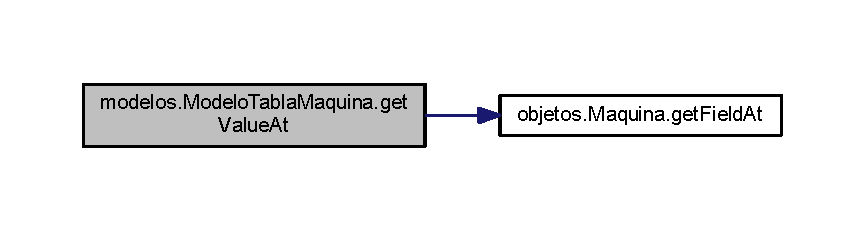
\includegraphics[width=350pt]{classmodelos_1_1_modelo_tabla_maquina_ae6611198ecf631949ddb041b8231da95_cgraph}
\end{center}
\end{figure}
\mbox{\Hypertarget{classmodelos_1_1_modelo_tabla_maquina_a76d930fbec2a211e91095ac641f030cb}\label{classmodelos_1_1_modelo_tabla_maquina_a76d930fbec2a211e91095ac641f030cb}} 
\index{modelos\+::\+Modelo\+Tabla\+Maquina@{modelos\+::\+Modelo\+Tabla\+Maquina}!get\+Value\+At2@{get\+Value\+At2}}
\index{get\+Value\+At2@{get\+Value\+At2}!modelos\+::\+Modelo\+Tabla\+Maquina@{modelos\+::\+Modelo\+Tabla\+Maquina}}
\subsubsection{\texorpdfstring{get\+Value\+At2()}{getValueAt2()}}
{\footnotesize\ttfamily Boolean modelos.\+Modelo\+Tabla\+Maquina.\+get\+Value\+At2 (\begin{DoxyParamCaption}\item[{int}]{fila,  }\item[{int}]{columna }\end{DoxyParamCaption})}



Definition at line 61 of file Modelo\+Tabla\+Maquina.\+java.

Here is the call graph for this function\+:
\nopagebreak
\begin{figure}[H]
\begin{center}
\leavevmode
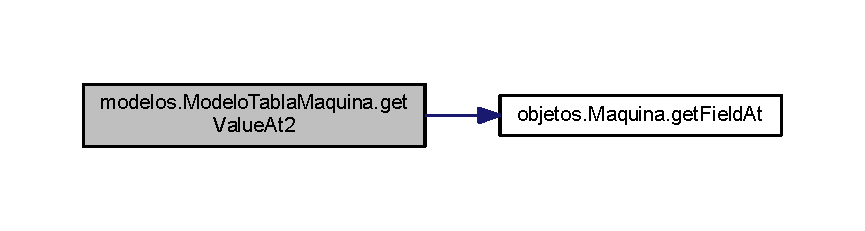
\includegraphics[width=350pt]{classmodelos_1_1_modelo_tabla_maquina_a76d930fbec2a211e91095ac641f030cb_cgraph}
\end{center}
\end{figure}
\mbox{\Hypertarget{classmodelos_1_1_modelo_tabla_maquina_ab81f2b02aa2cc4c0f9c93111ba345df8}\label{classmodelos_1_1_modelo_tabla_maquina_ab81f2b02aa2cc4c0f9c93111ba345df8}} 
\index{modelos\+::\+Modelo\+Tabla\+Maquina@{modelos\+::\+Modelo\+Tabla\+Maquina}!is\+Cell\+Editable@{is\+Cell\+Editable}}
\index{is\+Cell\+Editable@{is\+Cell\+Editable}!modelos\+::\+Modelo\+Tabla\+Maquina@{modelos\+::\+Modelo\+Tabla\+Maquina}}
\subsubsection{\texorpdfstring{is\+Cell\+Editable()}{isCellEditable()}}
{\footnotesize\ttfamily boolean modelos.\+Modelo\+Tabla\+Maquina.\+is\+Cell\+Editable (\begin{DoxyParamCaption}\item[{int}]{row\+Index,  }\item[{int}]{column\+Index }\end{DoxyParamCaption})}



Definition at line 79 of file Modelo\+Tabla\+Maquina.\+java.

\mbox{\Hypertarget{classmodelos_1_1_modelo_tabla_maquina_a48d1751bbb3bfb91d50eb5bd2a80207e}\label{classmodelos_1_1_modelo_tabla_maquina_a48d1751bbb3bfb91d50eb5bd2a80207e}} 
\index{modelos\+::\+Modelo\+Tabla\+Maquina@{modelos\+::\+Modelo\+Tabla\+Maquina}!refrescar\+Tabla@{refrescar\+Tabla}}
\index{refrescar\+Tabla@{refrescar\+Tabla}!modelos\+::\+Modelo\+Tabla\+Maquina@{modelos\+::\+Modelo\+Tabla\+Maquina}}
\subsubsection{\texorpdfstring{refrescar\+Tabla()}{refrescarTabla()}}
{\footnotesize\ttfamily void modelos.\+Modelo\+Tabla\+Maquina.\+refrescar\+Tabla (\begin{DoxyParamCaption}{ }\end{DoxyParamCaption})}



Definition at line 52 of file Modelo\+Tabla\+Maquina.\+java.

\mbox{\Hypertarget{classmodelos_1_1_modelo_tabla_maquina_a559a21bd653aa7b639fa598ff22fa5f7}\label{classmodelos_1_1_modelo_tabla_maquina_a559a21bd653aa7b639fa598ff22fa5f7}} 
\index{modelos\+::\+Modelo\+Tabla\+Maquina@{modelos\+::\+Modelo\+Tabla\+Maquina}!setlista\+Maquinas@{setlista\+Maquinas}}
\index{setlista\+Maquinas@{setlista\+Maquinas}!modelos\+::\+Modelo\+Tabla\+Maquina@{modelos\+::\+Modelo\+Tabla\+Maquina}}
\subsubsection{\texorpdfstring{setlista\+Maquinas()}{setlistaMaquinas()}}
{\footnotesize\ttfamily void modelos.\+Modelo\+Tabla\+Maquina.\+setlista\+Maquinas (\begin{DoxyParamCaption}\item[{List$<$ \mbox{\hyperlink{classobjetos_1_1_maquina}{Maquina}} $>$}]{lista\+Maquinas }\end{DoxyParamCaption})}



Definition at line 39 of file Modelo\+Tabla\+Maquina.\+java.



The documentation for this class was generated from the following file\+:\begin{DoxyCompactItemize}
\item 
C\+:/\+Users/jonmu/\+Desktop/\+P\+O\+P\+B\+L 4/src/modelos/\mbox{\hyperlink{_modelo_tabla_maquina_8java}{Modelo\+Tabla\+Maquina.\+java}}\end{DoxyCompactItemize}

\hypertarget{classmodelos_1_1_modelo_tabla_productos}{}\section{modelos.\+Modelo\+Tabla\+Productos Class Reference}
\label{classmodelos_1_1_modelo_tabla_productos}\index{modelos.\+Modelo\+Tabla\+Productos@{modelos.\+Modelo\+Tabla\+Productos}}


Inheritance diagram for modelos.\+Modelo\+Tabla\+Productos\+:\nopagebreak
\begin{figure}[H]
\begin{center}
\leavevmode
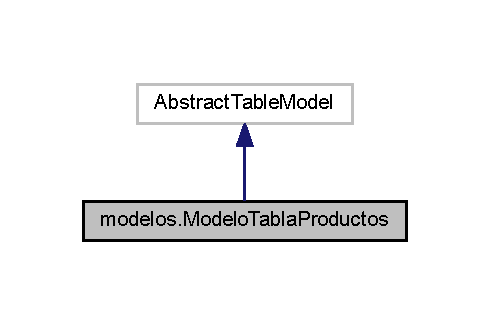
\includegraphics[width=235pt]{classmodelos_1_1_modelo_tabla_productos__inherit__graph}
\end{center}
\end{figure}


Collaboration diagram for modelos.\+Modelo\+Tabla\+Productos\+:\nopagebreak
\begin{figure}[H]
\begin{center}
\leavevmode
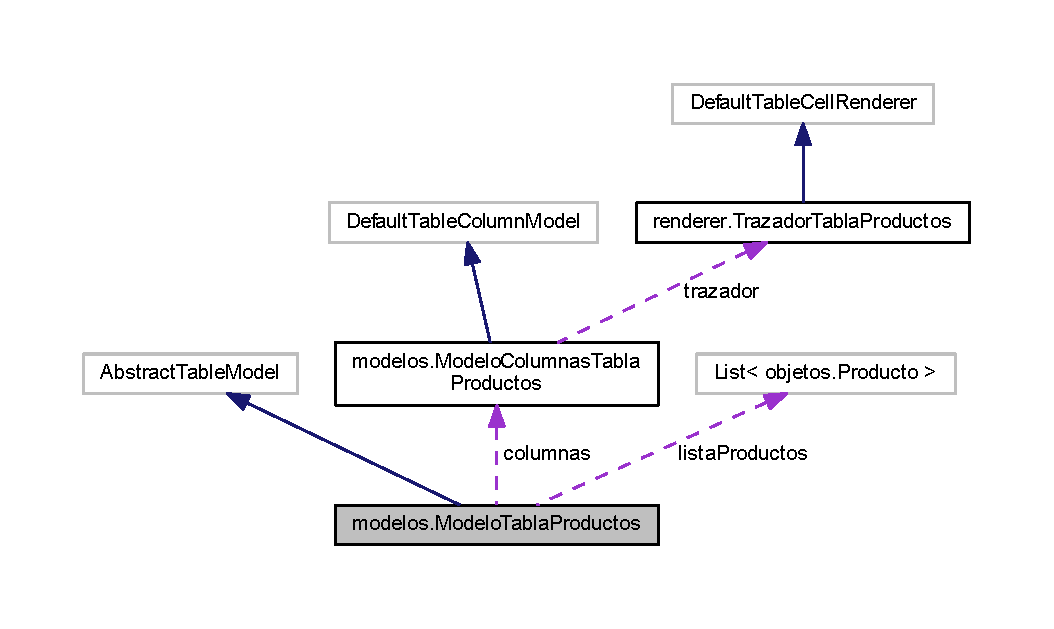
\includegraphics[width=350pt]{classmodelos_1_1_modelo_tabla_productos__coll__graph}
\end{center}
\end{figure}
\subsection*{Public Member Functions}
\begin{DoxyCompactItemize}
\item 
\mbox{\hyperlink{classmodelos_1_1_modelo_tabla_productos_ab5f5d0799330e203798a748c83667a9c}{Modelo\+Tabla\+Productos}} (\mbox{\hyperlink{classmodelos_1_1_modelo_columnas_tabla_productos}{Modelo\+Columnas\+Tabla\+Productos}} columnas)
\item 
void \mbox{\hyperlink{classmodelos_1_1_modelo_tabla_productos_ab0e461fbc9ca41944463eeeebf8a0625}{a�adir}} (\mbox{\hyperlink{classobjetos_1_1_producto}{Producto}} p)
\item 
void \mbox{\hyperlink{classmodelos_1_1_modelo_tabla_productos_af3b18a2452fc0a940ed50b2b7fb66141}{eliminar}} (int indice)
\item 
void \mbox{\hyperlink{classmodelos_1_1_modelo_tabla_productos_a70a7f512df5156d6b8a31f12afd8a570}{calcular\+Total}} ()
\item 
double \mbox{\hyperlink{classmodelos_1_1_modelo_tabla_productos_a731f5572c48b05c966a25ec8843d57cd}{get\+Suma\+Total}} ()
\item 
int \mbox{\hyperlink{classmodelos_1_1_modelo_tabla_productos_aa96dc58d192873c59a2f93019ae863fa}{get\+Row\+Count}} ()
\item 
Object \mbox{\hyperlink{classmodelos_1_1_modelo_tabla_productos_a4c91c243cd2d6689592284213fceaa0b}{get\+Value\+At}} (int fila, int columna)
\item 
boolean \mbox{\hyperlink{classmodelos_1_1_modelo_tabla_productos_adcb2c78b3c808f116830f02f84afb2c7}{is\+Cell\+Editable}} (int row\+Index, int column\+Index)
\item 
Class$<$?$>$ \mbox{\hyperlink{classmodelos_1_1_modelo_tabla_productos_a026132fca397cfb0fe320cc6dc7fbf3d}{get\+Column\+Class}} (int column\+Index)
\item 
int \mbox{\hyperlink{classmodelos_1_1_modelo_tabla_productos_ac56966c494669df1ea4a61da25cb75d3}{get\+Column\+Count}} ()
\item 
void \mbox{\hyperlink{classmodelos_1_1_modelo_tabla_productos_a24e1a6fceb277de8501c5410125d27ca}{set\+Lista\+Productos}} (\mbox{\hyperlink{classobjetos_1_1_pedido}{Pedido}} p)
\item 
List$<$ \mbox{\hyperlink{classobjetos_1_1_producto}{Producto}} $>$ \mbox{\hyperlink{classmodelos_1_1_modelo_tabla_productos_ac85802b2d07288879883d1826e2d7bd3}{get\+Lista\+Productos}} ()
\end{DoxyCompactItemize}


\subsection{Detailed Description}


Definition at line 12 of file Modelo\+Tabla\+Productos.\+java.



\subsection{Constructor \& Destructor Documentation}
\mbox{\Hypertarget{classmodelos_1_1_modelo_tabla_productos_ab5f5d0799330e203798a748c83667a9c}\label{classmodelos_1_1_modelo_tabla_productos_ab5f5d0799330e203798a748c83667a9c}} 
\index{modelos\+::\+Modelo\+Tabla\+Productos@{modelos\+::\+Modelo\+Tabla\+Productos}!Modelo\+Tabla\+Productos@{Modelo\+Tabla\+Productos}}
\index{Modelo\+Tabla\+Productos@{Modelo\+Tabla\+Productos}!modelos\+::\+Modelo\+Tabla\+Productos@{modelos\+::\+Modelo\+Tabla\+Productos}}
\subsubsection{\texorpdfstring{Modelo\+Tabla\+Productos()}{ModeloTablaProductos()}}
{\footnotesize\ttfamily modelos.\+Modelo\+Tabla\+Productos.\+Modelo\+Tabla\+Productos (\begin{DoxyParamCaption}\item[{\mbox{\hyperlink{classmodelos_1_1_modelo_columnas_tabla_productos}{Modelo\+Columnas\+Tabla\+Productos}}}]{columnas }\end{DoxyParamCaption})}



Definition at line 23 of file Modelo\+Tabla\+Productos.\+java.



\subsection{Member Function Documentation}
\mbox{\Hypertarget{classmodelos_1_1_modelo_tabla_productos_ab0e461fbc9ca41944463eeeebf8a0625}\label{classmodelos_1_1_modelo_tabla_productos_ab0e461fbc9ca41944463eeeebf8a0625}} 
\index{modelos\+::\+Modelo\+Tabla\+Productos@{modelos\+::\+Modelo\+Tabla\+Productos}!a�adir@{a�adir}}
\index{a�adir@{a�adir}!modelos\+::\+Modelo\+Tabla\+Productos@{modelos\+::\+Modelo\+Tabla\+Productos}}
\subsubsection{\texorpdfstring{a�adir()}{a�adir()}}
{\footnotesize\ttfamily void modelos.\+Modelo\+Tabla\+Productos.\+a�adir (\begin{DoxyParamCaption}\item[{\mbox{\hyperlink{classobjetos_1_1_producto}{Producto}}}]{p }\end{DoxyParamCaption})}



Definition at line 30 of file Modelo\+Tabla\+Productos.\+java.

\mbox{\Hypertarget{classmodelos_1_1_modelo_tabla_productos_a70a7f512df5156d6b8a31f12afd8a570}\label{classmodelos_1_1_modelo_tabla_productos_a70a7f512df5156d6b8a31f12afd8a570}} 
\index{modelos\+::\+Modelo\+Tabla\+Productos@{modelos\+::\+Modelo\+Tabla\+Productos}!calcular\+Total@{calcular\+Total}}
\index{calcular\+Total@{calcular\+Total}!modelos\+::\+Modelo\+Tabla\+Productos@{modelos\+::\+Modelo\+Tabla\+Productos}}
\subsubsection{\texorpdfstring{calcular\+Total()}{calcularTotal()}}
{\footnotesize\ttfamily void modelos.\+Modelo\+Tabla\+Productos.\+calcular\+Total (\begin{DoxyParamCaption}{ }\end{DoxyParamCaption})}



Definition at line 41 of file Modelo\+Tabla\+Productos.\+java.

\mbox{\Hypertarget{classmodelos_1_1_modelo_tabla_productos_af3b18a2452fc0a940ed50b2b7fb66141}\label{classmodelos_1_1_modelo_tabla_productos_af3b18a2452fc0a940ed50b2b7fb66141}} 
\index{modelos\+::\+Modelo\+Tabla\+Productos@{modelos\+::\+Modelo\+Tabla\+Productos}!eliminar@{eliminar}}
\index{eliminar@{eliminar}!modelos\+::\+Modelo\+Tabla\+Productos@{modelos\+::\+Modelo\+Tabla\+Productos}}
\subsubsection{\texorpdfstring{eliminar()}{eliminar()}}
{\footnotesize\ttfamily void modelos.\+Modelo\+Tabla\+Productos.\+eliminar (\begin{DoxyParamCaption}\item[{int}]{indice }\end{DoxyParamCaption})}



Definition at line 35 of file Modelo\+Tabla\+Productos.\+java.

\mbox{\Hypertarget{classmodelos_1_1_modelo_tabla_productos_a026132fca397cfb0fe320cc6dc7fbf3d}\label{classmodelos_1_1_modelo_tabla_productos_a026132fca397cfb0fe320cc6dc7fbf3d}} 
\index{modelos\+::\+Modelo\+Tabla\+Productos@{modelos\+::\+Modelo\+Tabla\+Productos}!get\+Column\+Class@{get\+Column\+Class}}
\index{get\+Column\+Class@{get\+Column\+Class}!modelos\+::\+Modelo\+Tabla\+Productos@{modelos\+::\+Modelo\+Tabla\+Productos}}
\subsubsection{\texorpdfstring{get\+Column\+Class()}{getColumnClass()}}
{\footnotesize\ttfamily Class$<$?$>$ modelos.\+Modelo\+Tabla\+Productos.\+get\+Column\+Class (\begin{DoxyParamCaption}\item[{int}]{column\+Index }\end{DoxyParamCaption})}



Definition at line 70 of file Modelo\+Tabla\+Productos.\+java.

Here is the call graph for this function\+:\nopagebreak
\begin{figure}[H]
\begin{center}
\leavevmode
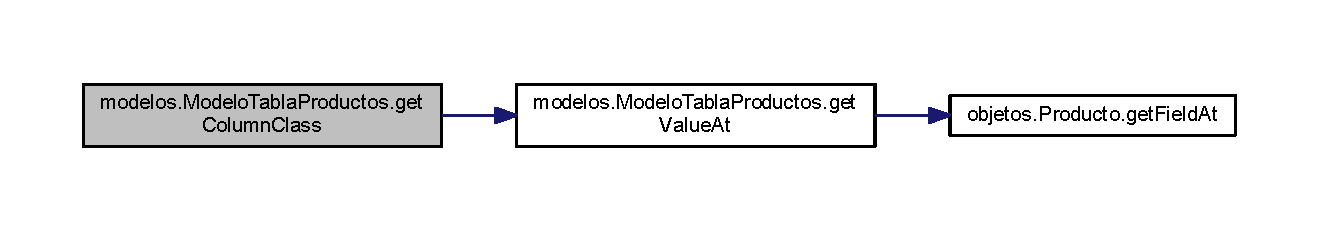
\includegraphics[width=350pt]{classmodelos_1_1_modelo_tabla_productos_a026132fca397cfb0fe320cc6dc7fbf3d_cgraph}
\end{center}
\end{figure}
\mbox{\Hypertarget{classmodelos_1_1_modelo_tabla_productos_ac56966c494669df1ea4a61da25cb75d3}\label{classmodelos_1_1_modelo_tabla_productos_ac56966c494669df1ea4a61da25cb75d3}} 
\index{modelos\+::\+Modelo\+Tabla\+Productos@{modelos\+::\+Modelo\+Tabla\+Productos}!get\+Column\+Count@{get\+Column\+Count}}
\index{get\+Column\+Count@{get\+Column\+Count}!modelos\+::\+Modelo\+Tabla\+Productos@{modelos\+::\+Modelo\+Tabla\+Productos}}
\subsubsection{\texorpdfstring{get\+Column\+Count()}{getColumnCount()}}
{\footnotesize\ttfamily int modelos.\+Modelo\+Tabla\+Productos.\+get\+Column\+Count (\begin{DoxyParamCaption}{ }\end{DoxyParamCaption})}



Definition at line 75 of file Modelo\+Tabla\+Productos.\+java.

\mbox{\Hypertarget{classmodelos_1_1_modelo_tabla_productos_ac85802b2d07288879883d1826e2d7bd3}\label{classmodelos_1_1_modelo_tabla_productos_ac85802b2d07288879883d1826e2d7bd3}} 
\index{modelos\+::\+Modelo\+Tabla\+Productos@{modelos\+::\+Modelo\+Tabla\+Productos}!get\+Lista\+Productos@{get\+Lista\+Productos}}
\index{get\+Lista\+Productos@{get\+Lista\+Productos}!modelos\+::\+Modelo\+Tabla\+Productos@{modelos\+::\+Modelo\+Tabla\+Productos}}
\subsubsection{\texorpdfstring{get\+Lista\+Productos()}{getListaProductos()}}
{\footnotesize\ttfamily List$<$\mbox{\hyperlink{classobjetos_1_1_producto}{Producto}}$>$ modelos.\+Modelo\+Tabla\+Productos.\+get\+Lista\+Productos (\begin{DoxyParamCaption}{ }\end{DoxyParamCaption})}



Definition at line 84 of file Modelo\+Tabla\+Productos.\+java.

\mbox{\Hypertarget{classmodelos_1_1_modelo_tabla_productos_aa96dc58d192873c59a2f93019ae863fa}\label{classmodelos_1_1_modelo_tabla_productos_aa96dc58d192873c59a2f93019ae863fa}} 
\index{modelos\+::\+Modelo\+Tabla\+Productos@{modelos\+::\+Modelo\+Tabla\+Productos}!get\+Row\+Count@{get\+Row\+Count}}
\index{get\+Row\+Count@{get\+Row\+Count}!modelos\+::\+Modelo\+Tabla\+Productos@{modelos\+::\+Modelo\+Tabla\+Productos}}
\subsubsection{\texorpdfstring{get\+Row\+Count()}{getRowCount()}}
{\footnotesize\ttfamily int modelos.\+Modelo\+Tabla\+Productos.\+get\+Row\+Count (\begin{DoxyParamCaption}{ }\end{DoxyParamCaption})}



Definition at line 54 of file Modelo\+Tabla\+Productos.\+java.

\mbox{\Hypertarget{classmodelos_1_1_modelo_tabla_productos_a731f5572c48b05c966a25ec8843d57cd}\label{classmodelos_1_1_modelo_tabla_productos_a731f5572c48b05c966a25ec8843d57cd}} 
\index{modelos\+::\+Modelo\+Tabla\+Productos@{modelos\+::\+Modelo\+Tabla\+Productos}!get\+Suma\+Total@{get\+Suma\+Total}}
\index{get\+Suma\+Total@{get\+Suma\+Total}!modelos\+::\+Modelo\+Tabla\+Productos@{modelos\+::\+Modelo\+Tabla\+Productos}}
\subsubsection{\texorpdfstring{get\+Suma\+Total()}{getSumaTotal()}}
{\footnotesize\ttfamily double modelos.\+Modelo\+Tabla\+Productos.\+get\+Suma\+Total (\begin{DoxyParamCaption}{ }\end{DoxyParamCaption})}



Definition at line 49 of file Modelo\+Tabla\+Productos.\+java.

\mbox{\Hypertarget{classmodelos_1_1_modelo_tabla_productos_a4c91c243cd2d6689592284213fceaa0b}\label{classmodelos_1_1_modelo_tabla_productos_a4c91c243cd2d6689592284213fceaa0b}} 
\index{modelos\+::\+Modelo\+Tabla\+Productos@{modelos\+::\+Modelo\+Tabla\+Productos}!get\+Value\+At@{get\+Value\+At}}
\index{get\+Value\+At@{get\+Value\+At}!modelos\+::\+Modelo\+Tabla\+Productos@{modelos\+::\+Modelo\+Tabla\+Productos}}
\subsubsection{\texorpdfstring{get\+Value\+At()}{getValueAt()}}
{\footnotesize\ttfamily Object modelos.\+Modelo\+Tabla\+Productos.\+get\+Value\+At (\begin{DoxyParamCaption}\item[{int}]{fila,  }\item[{int}]{columna }\end{DoxyParamCaption})}



Definition at line 59 of file Modelo\+Tabla\+Productos.\+java.

Here is the call graph for this function\+:\nopagebreak
\begin{figure}[H]
\begin{center}
\leavevmode
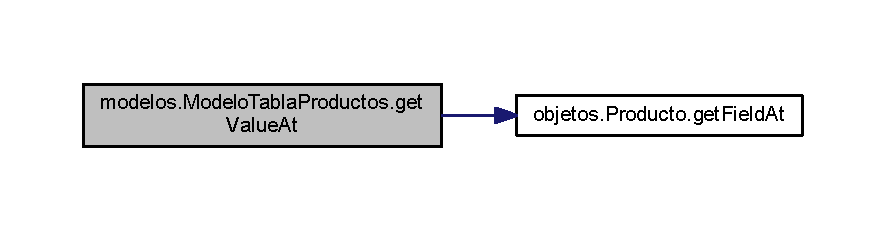
\includegraphics[width=350pt]{classmodelos_1_1_modelo_tabla_productos_a4c91c243cd2d6689592284213fceaa0b_cgraph}
\end{center}
\end{figure}
\mbox{\Hypertarget{classmodelos_1_1_modelo_tabla_productos_adcb2c78b3c808f116830f02f84afb2c7}\label{classmodelos_1_1_modelo_tabla_productos_adcb2c78b3c808f116830f02f84afb2c7}} 
\index{modelos\+::\+Modelo\+Tabla\+Productos@{modelos\+::\+Modelo\+Tabla\+Productos}!is\+Cell\+Editable@{is\+Cell\+Editable}}
\index{is\+Cell\+Editable@{is\+Cell\+Editable}!modelos\+::\+Modelo\+Tabla\+Productos@{modelos\+::\+Modelo\+Tabla\+Productos}}
\subsubsection{\texorpdfstring{is\+Cell\+Editable()}{isCellEditable()}}
{\footnotesize\ttfamily boolean modelos.\+Modelo\+Tabla\+Productos.\+is\+Cell\+Editable (\begin{DoxyParamCaption}\item[{int}]{row\+Index,  }\item[{int}]{column\+Index }\end{DoxyParamCaption})}



Definition at line 65 of file Modelo\+Tabla\+Productos.\+java.

\mbox{\Hypertarget{classmodelos_1_1_modelo_tabla_productos_a24e1a6fceb277de8501c5410125d27ca}\label{classmodelos_1_1_modelo_tabla_productos_a24e1a6fceb277de8501c5410125d27ca}} 
\index{modelos\+::\+Modelo\+Tabla\+Productos@{modelos\+::\+Modelo\+Tabla\+Productos}!set\+Lista\+Productos@{set\+Lista\+Productos}}
\index{set\+Lista\+Productos@{set\+Lista\+Productos}!modelos\+::\+Modelo\+Tabla\+Productos@{modelos\+::\+Modelo\+Tabla\+Productos}}
\subsubsection{\texorpdfstring{set\+Lista\+Productos()}{setListaProductos()}}
{\footnotesize\ttfamily void modelos.\+Modelo\+Tabla\+Productos.\+set\+Lista\+Productos (\begin{DoxyParamCaption}\item[{\mbox{\hyperlink{classobjetos_1_1_pedido}{Pedido}}}]{p }\end{DoxyParamCaption})}



Definition at line 79 of file Modelo\+Tabla\+Productos.\+java.

Here is the call graph for this function\+:\nopagebreak
\begin{figure}[H]
\begin{center}
\leavevmode
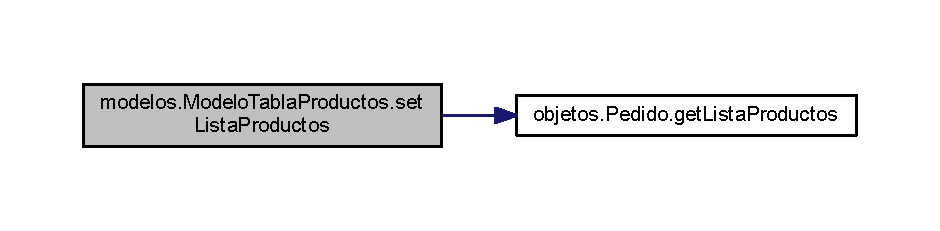
\includegraphics[width=350pt]{classmodelos_1_1_modelo_tabla_productos_a24e1a6fceb277de8501c5410125d27ca_cgraph}
\end{center}
\end{figure}


The documentation for this class was generated from the following file\+:\begin{DoxyCompactItemize}
\item 
C\+:/\+Users/jonmu/\+Desktop/\+P\+O\+P\+B\+L 4/src/modelos/\mbox{\hyperlink{_modelo_tabla_productos_8java}{Modelo\+Tabla\+Productos.\+java}}\end{DoxyCompactItemize}

\hypertarget{classmodelos_1_1_modelo_usuarios}{}\section{modelos.\+Modelo\+Usuarios Class Reference}
\label{classmodelos_1_1_modelo_usuarios}\index{modelos.\+Modelo\+Usuarios@{modelos.\+Modelo\+Usuarios}}


Inheritance diagram for modelos.\+Modelo\+Usuarios\+:
\nopagebreak
\begin{figure}[H]
\begin{center}
\leavevmode
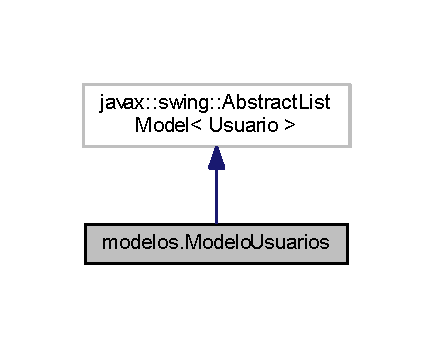
\includegraphics[width=208pt]{classmodelos_1_1_modelo_usuarios__inherit__graph}
\end{center}
\end{figure}


Collaboration diagram for modelos.\+Modelo\+Usuarios\+:
\nopagebreak
\begin{figure}[H]
\begin{center}
\leavevmode
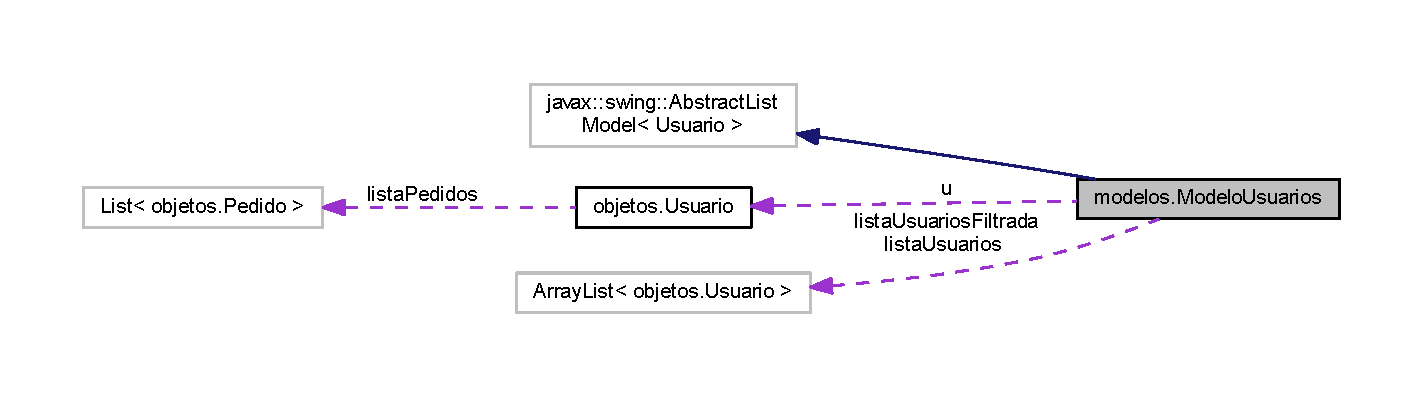
\includegraphics[width=350pt]{classmodelos_1_1_modelo_usuarios__coll__graph}
\end{center}
\end{figure}
\subsection*{Public Member Functions}
\begin{DoxyCompactItemize}
\item 
\mbox{\hyperlink{classmodelos_1_1_modelo_usuarios_a29eb753e9f246c911e679e28a7ba7173}{Modelo\+Usuarios}} (Array\+List$<$ \mbox{\hyperlink{classobjetos_1_1_usuario}{Usuario}} $>$ lista\+Usuarios)
\item 
void \mbox{\hyperlink{classmodelos_1_1_modelo_usuarios_a43fe9d71b2cb14a67af32df76c93f1ec}{filtrar\+Por\+Usuario}} (String filtro)
\item 
void \mbox{\hyperlink{classmodelos_1_1_modelo_usuarios_a32302d42fef716e596f45c6ed27a3641}{filtrar\+Por\+Codigo\+Postal}} (String filtro)
\item 
void \mbox{\hyperlink{classmodelos_1_1_modelo_usuarios_aa19c41161c68beb4f84f553bd3cca8b3}{filtrar\+Por\+Poblacion}} (String filtro)
\item 
void \mbox{\hyperlink{classmodelos_1_1_modelo_usuarios_a319bbe3d654caccba263e75ae64e9f37}{mostrar\+Todos}} ()
\item 
void \mbox{\hyperlink{classmodelos_1_1_modelo_usuarios_a65777b1abda04e3dd05762d1e5a4cc1d}{filtrar\+Por\+Dni}} (String filtro)
\item 
int \mbox{\hyperlink{classmodelos_1_1_modelo_usuarios_a35b3ac033cacc65073296b297d92eb0b}{get\+Size}} ()
\item 
\mbox{\hyperlink{classobjetos_1_1_usuario}{Usuario}} \mbox{\hyperlink{classmodelos_1_1_modelo_usuarios_ae477676a4f06527dc6f70b160ab5f426}{get\+Element\+At}} (int index)
\end{DoxyCompactItemize}


\subsection{Detailed Description}


Definition at line 13 of file Modelo\+Usuarios.\+java.



\subsection{Constructor \& Destructor Documentation}
\mbox{\Hypertarget{classmodelos_1_1_modelo_usuarios_a29eb753e9f246c911e679e28a7ba7173}\label{classmodelos_1_1_modelo_usuarios_a29eb753e9f246c911e679e28a7ba7173}} 
\index{modelos\+::\+Modelo\+Usuarios@{modelos\+::\+Modelo\+Usuarios}!Modelo\+Usuarios@{Modelo\+Usuarios}}
\index{Modelo\+Usuarios@{Modelo\+Usuarios}!modelos\+::\+Modelo\+Usuarios@{modelos\+::\+Modelo\+Usuarios}}
\subsubsection{\texorpdfstring{Modelo\+Usuarios()}{ModeloUsuarios()}}
{\footnotesize\ttfamily modelos.\+Modelo\+Usuarios.\+Modelo\+Usuarios (\begin{DoxyParamCaption}\item[{Array\+List$<$ \mbox{\hyperlink{classobjetos_1_1_usuario}{Usuario}} $>$}]{lista\+Usuarios }\end{DoxyParamCaption})}



Definition at line 24 of file Modelo\+Usuarios.\+java.



\subsection{Member Function Documentation}
\mbox{\Hypertarget{classmodelos_1_1_modelo_usuarios_a32302d42fef716e596f45c6ed27a3641}\label{classmodelos_1_1_modelo_usuarios_a32302d42fef716e596f45c6ed27a3641}} 
\index{modelos\+::\+Modelo\+Usuarios@{modelos\+::\+Modelo\+Usuarios}!filtrar\+Por\+Codigo\+Postal@{filtrar\+Por\+Codigo\+Postal}}
\index{filtrar\+Por\+Codigo\+Postal@{filtrar\+Por\+Codigo\+Postal}!modelos\+::\+Modelo\+Usuarios@{modelos\+::\+Modelo\+Usuarios}}
\subsubsection{\texorpdfstring{filtrar\+Por\+Codigo\+Postal()}{filtrarPorCodigoPostal()}}
{\footnotesize\ttfamily void modelos.\+Modelo\+Usuarios.\+filtrar\+Por\+Codigo\+Postal (\begin{DoxyParamCaption}\item[{String}]{filtro }\end{DoxyParamCaption})}



Definition at line 42 of file Modelo\+Usuarios.\+java.

\mbox{\Hypertarget{classmodelos_1_1_modelo_usuarios_a65777b1abda04e3dd05762d1e5a4cc1d}\label{classmodelos_1_1_modelo_usuarios_a65777b1abda04e3dd05762d1e5a4cc1d}} 
\index{modelos\+::\+Modelo\+Usuarios@{modelos\+::\+Modelo\+Usuarios}!filtrar\+Por\+Dni@{filtrar\+Por\+Dni}}
\index{filtrar\+Por\+Dni@{filtrar\+Por\+Dni}!modelos\+::\+Modelo\+Usuarios@{modelos\+::\+Modelo\+Usuarios}}
\subsubsection{\texorpdfstring{filtrar\+Por\+Dni()}{filtrarPorDni()}}
{\footnotesize\ttfamily void modelos.\+Modelo\+Usuarios.\+filtrar\+Por\+Dni (\begin{DoxyParamCaption}\item[{String}]{filtro }\end{DoxyParamCaption})}



Definition at line 67 of file Modelo\+Usuarios.\+java.

\mbox{\Hypertarget{classmodelos_1_1_modelo_usuarios_aa19c41161c68beb4f84f553bd3cca8b3}\label{classmodelos_1_1_modelo_usuarios_aa19c41161c68beb4f84f553bd3cca8b3}} 
\index{modelos\+::\+Modelo\+Usuarios@{modelos\+::\+Modelo\+Usuarios}!filtrar\+Por\+Poblacion@{filtrar\+Por\+Poblacion}}
\index{filtrar\+Por\+Poblacion@{filtrar\+Por\+Poblacion}!modelos\+::\+Modelo\+Usuarios@{modelos\+::\+Modelo\+Usuarios}}
\subsubsection{\texorpdfstring{filtrar\+Por\+Poblacion()}{filtrarPorPoblacion()}}
{\footnotesize\ttfamily void modelos.\+Modelo\+Usuarios.\+filtrar\+Por\+Poblacion (\begin{DoxyParamCaption}\item[{String}]{filtro }\end{DoxyParamCaption})}



Definition at line 50 of file Modelo\+Usuarios.\+java.

\mbox{\Hypertarget{classmodelos_1_1_modelo_usuarios_a43fe9d71b2cb14a67af32df76c93f1ec}\label{classmodelos_1_1_modelo_usuarios_a43fe9d71b2cb14a67af32df76c93f1ec}} 
\index{modelos\+::\+Modelo\+Usuarios@{modelos\+::\+Modelo\+Usuarios}!filtrar\+Por\+Usuario@{filtrar\+Por\+Usuario}}
\index{filtrar\+Por\+Usuario@{filtrar\+Por\+Usuario}!modelos\+::\+Modelo\+Usuarios@{modelos\+::\+Modelo\+Usuarios}}
\subsubsection{\texorpdfstring{filtrar\+Por\+Usuario()}{filtrarPorUsuario()}}
{\footnotesize\ttfamily void modelos.\+Modelo\+Usuarios.\+filtrar\+Por\+Usuario (\begin{DoxyParamCaption}\item[{String}]{filtro }\end{DoxyParamCaption})}



Definition at line 33 of file Modelo\+Usuarios.\+java.

\mbox{\Hypertarget{classmodelos_1_1_modelo_usuarios_ae477676a4f06527dc6f70b160ab5f426}\label{classmodelos_1_1_modelo_usuarios_ae477676a4f06527dc6f70b160ab5f426}} 
\index{modelos\+::\+Modelo\+Usuarios@{modelos\+::\+Modelo\+Usuarios}!get\+Element\+At@{get\+Element\+At}}
\index{get\+Element\+At@{get\+Element\+At}!modelos\+::\+Modelo\+Usuarios@{modelos\+::\+Modelo\+Usuarios}}
\subsubsection{\texorpdfstring{get\+Element\+At()}{getElementAt()}}
{\footnotesize\ttfamily \mbox{\hyperlink{classobjetos_1_1_usuario}{Usuario}} modelos.\+Modelo\+Usuarios.\+get\+Element\+At (\begin{DoxyParamCaption}\item[{int}]{index }\end{DoxyParamCaption})}



Definition at line 81 of file Modelo\+Usuarios.\+java.

\mbox{\Hypertarget{classmodelos_1_1_modelo_usuarios_a35b3ac033cacc65073296b297d92eb0b}\label{classmodelos_1_1_modelo_usuarios_a35b3ac033cacc65073296b297d92eb0b}} 
\index{modelos\+::\+Modelo\+Usuarios@{modelos\+::\+Modelo\+Usuarios}!get\+Size@{get\+Size}}
\index{get\+Size@{get\+Size}!modelos\+::\+Modelo\+Usuarios@{modelos\+::\+Modelo\+Usuarios}}
\subsubsection{\texorpdfstring{get\+Size()}{getSize()}}
{\footnotesize\ttfamily int modelos.\+Modelo\+Usuarios.\+get\+Size (\begin{DoxyParamCaption}{ }\end{DoxyParamCaption})}



Definition at line 76 of file Modelo\+Usuarios.\+java.

\mbox{\Hypertarget{classmodelos_1_1_modelo_usuarios_a319bbe3d654caccba263e75ae64e9f37}\label{classmodelos_1_1_modelo_usuarios_a319bbe3d654caccba263e75ae64e9f37}} 
\index{modelos\+::\+Modelo\+Usuarios@{modelos\+::\+Modelo\+Usuarios}!mostrar\+Todos@{mostrar\+Todos}}
\index{mostrar\+Todos@{mostrar\+Todos}!modelos\+::\+Modelo\+Usuarios@{modelos\+::\+Modelo\+Usuarios}}
\subsubsection{\texorpdfstring{mostrar\+Todos()}{mostrarTodos()}}
{\footnotesize\ttfamily void modelos.\+Modelo\+Usuarios.\+mostrar\+Todos (\begin{DoxyParamCaption}{ }\end{DoxyParamCaption})}



Definition at line 58 of file Modelo\+Usuarios.\+java.



The documentation for this class was generated from the following file\+:\begin{DoxyCompactItemize}
\item 
C\+:/\+Users/jonmu/\+Desktop/\+P\+O\+P\+B\+L 4/src/modelos/\mbox{\hyperlink{_modelo_usuarios_8java}{Modelo\+Usuarios.\+java}}\end{DoxyCompactItemize}

\hypertarget{classpaneles_1_1_panel_acceso}{}\section{paneles.\+Panel\+Acceso Class Reference}
\label{classpaneles_1_1_panel_acceso}\index{paneles.\+Panel\+Acceso@{paneles.\+Panel\+Acceso}}


Collaboration diagram for paneles.\+Panel\+Acceso\+:
\nopagebreak
\begin{figure}[H]
\begin{center}
\leavevmode
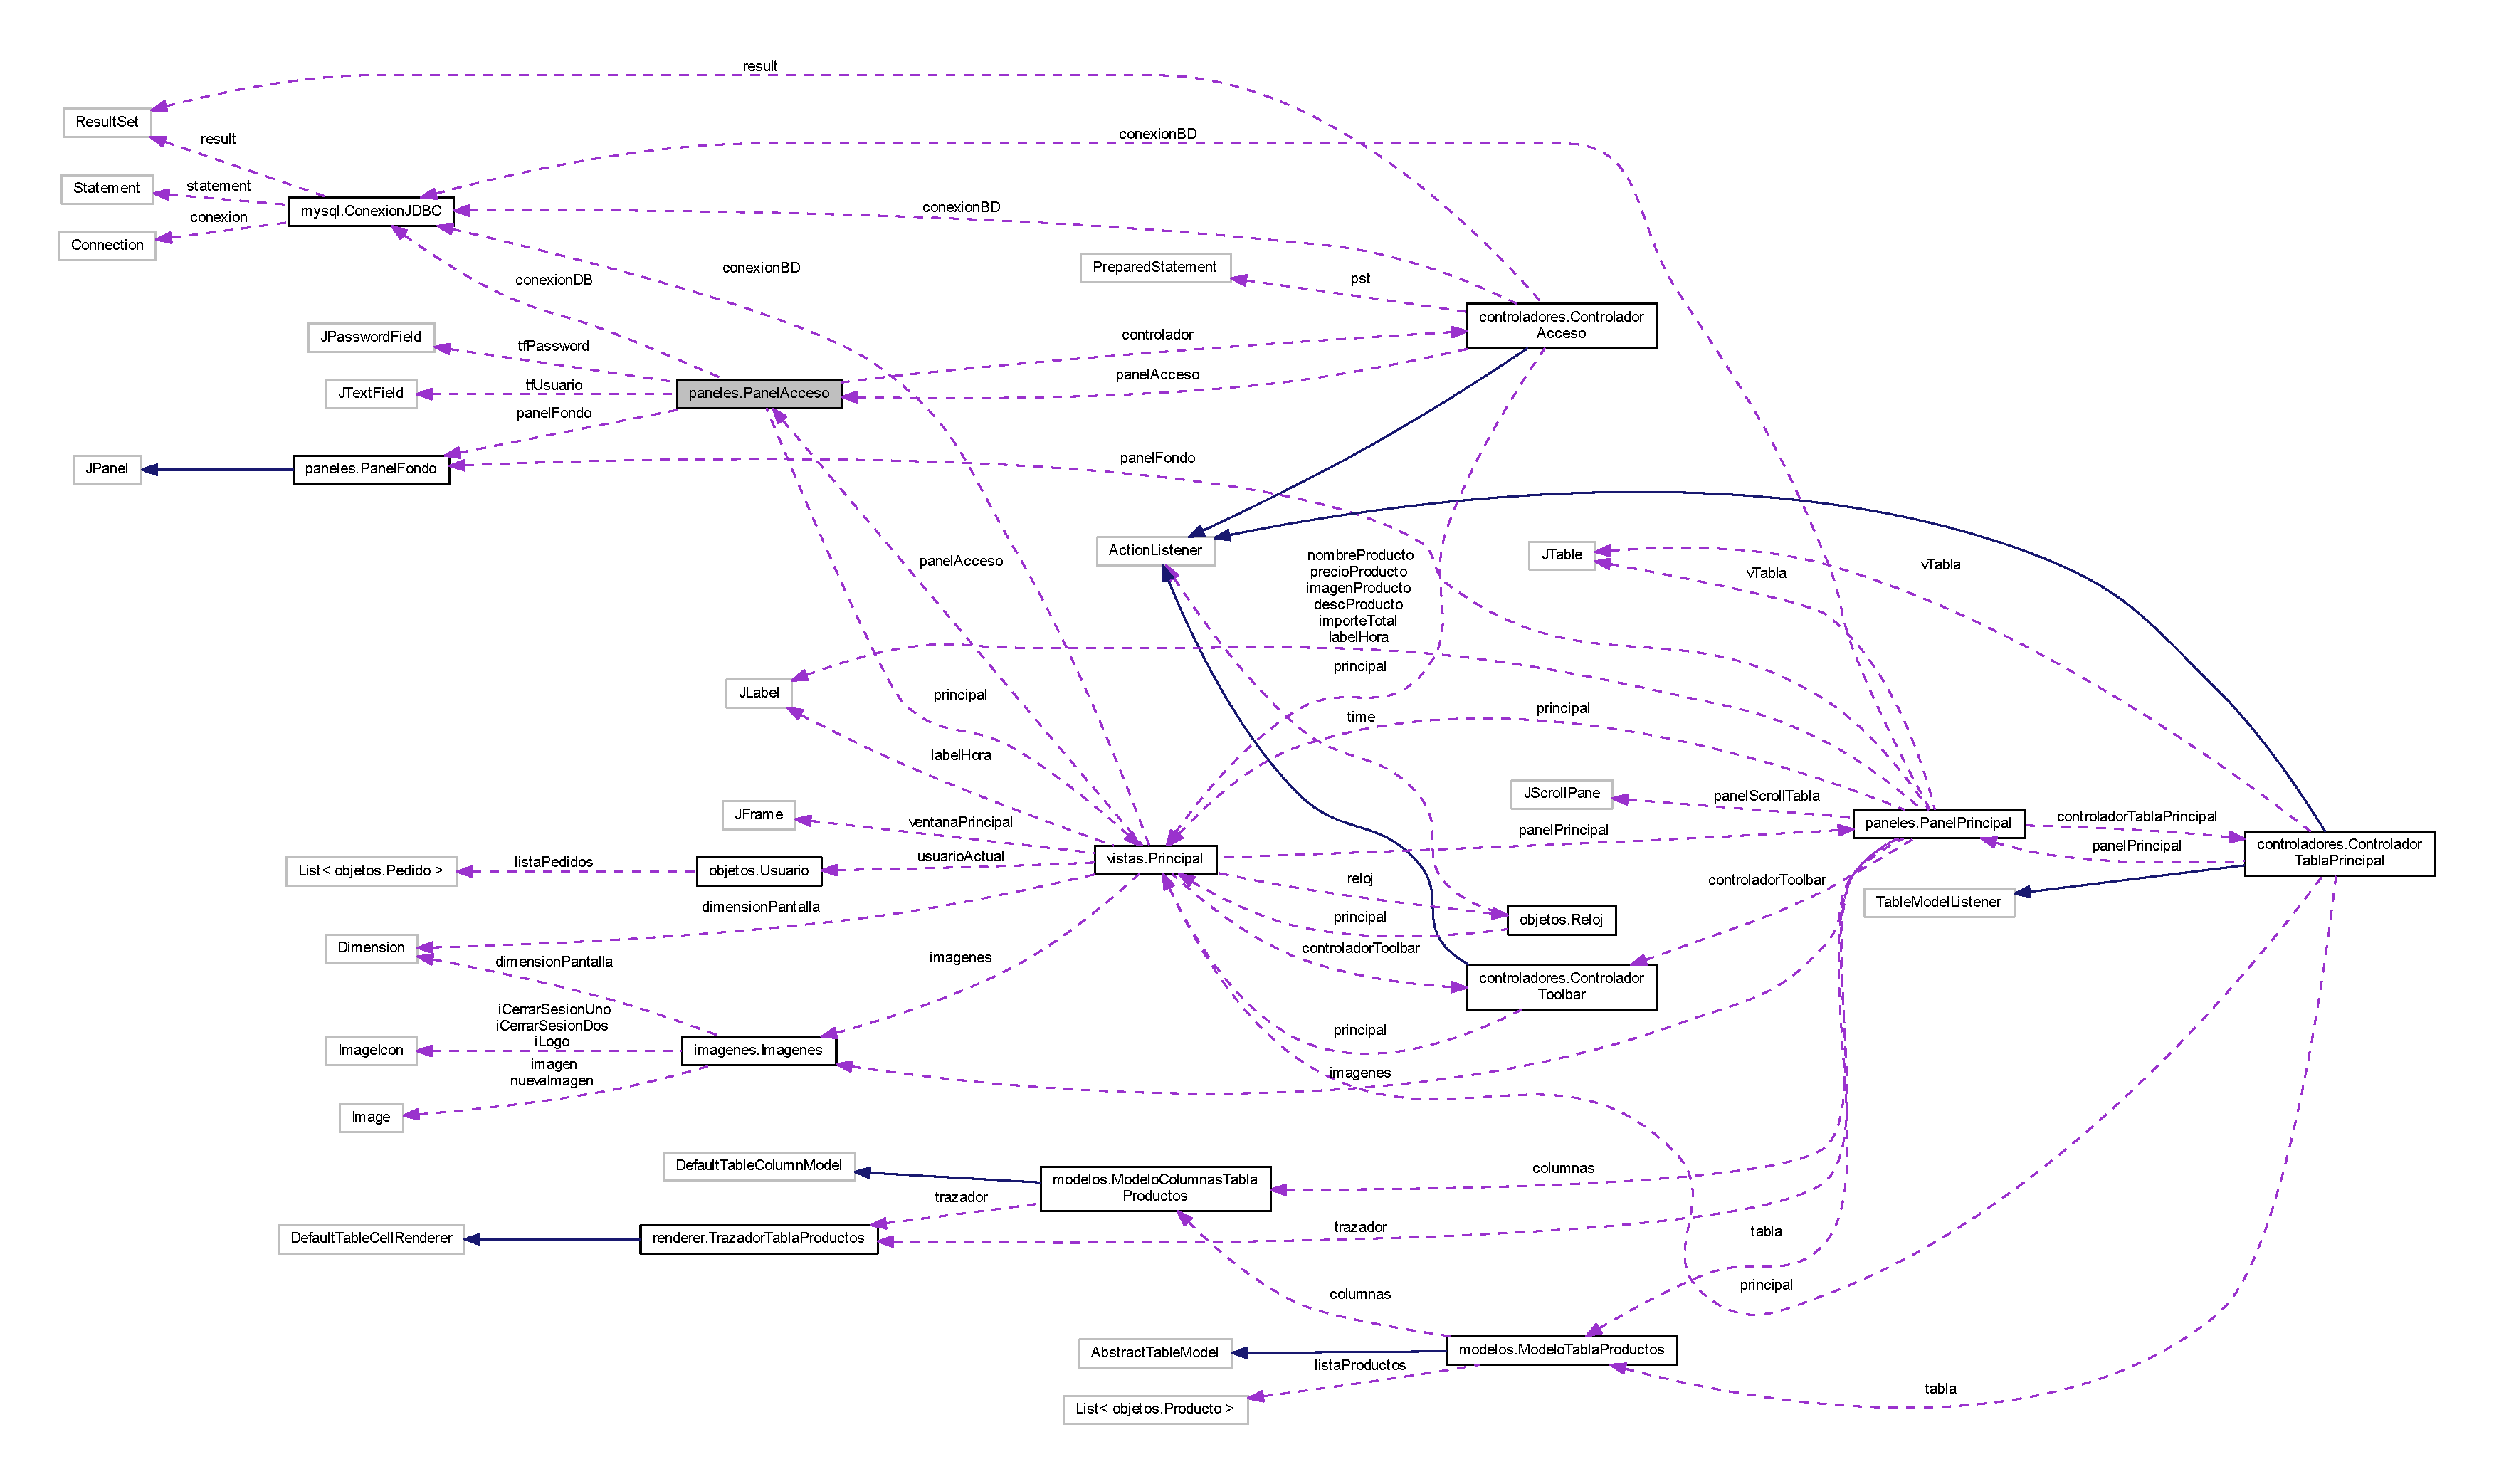
\includegraphics[width=350pt]{classpaneles_1_1_panel_acceso__coll__graph}
\end{center}
\end{figure}
\subsection*{Public Member Functions}
\begin{DoxyCompactItemize}
\item 
\mbox{\hyperlink{classpaneles_1_1_panel_acceso_ab19590219a09f461529209808b8dbd25}{Panel\+Acceso}} (\mbox{\hyperlink{classvistas_1_1_principal}{Principal}} principal, \mbox{\hyperlink{classmysql_1_1_conexion_j_d_b_c}{Conexion\+J\+D\+BC}} conexion\+DB)
\item 
J\+Panel \mbox{\hyperlink{classpaneles_1_1_panel_acceso_ac978a2c0e1aef22aa66b19abe354b02b}{get\+Panel}} ()
\item 
J\+Text\+Field \mbox{\hyperlink{classpaneles_1_1_panel_acceso_a2e9e57df2c86935dcee9830931a7d3ec}{get\+Tf\+Usuario}} ()
\item 
J\+Password\+Field \mbox{\hyperlink{classpaneles_1_1_panel_acceso_acff0ecd448fa0435276817069e088492}{get\+Tf\+Password}} ()
\end{DoxyCompactItemize}


\subsection{Detailed Description}


Definition at line 25 of file Panel\+Acceso.\+java.



\subsection{Constructor \& Destructor Documentation}
\mbox{\Hypertarget{classpaneles_1_1_panel_acceso_ab19590219a09f461529209808b8dbd25}\label{classpaneles_1_1_panel_acceso_ab19590219a09f461529209808b8dbd25}} 
\index{paneles\+::\+Panel\+Acceso@{paneles\+::\+Panel\+Acceso}!Panel\+Acceso@{Panel\+Acceso}}
\index{Panel\+Acceso@{Panel\+Acceso}!paneles\+::\+Panel\+Acceso@{paneles\+::\+Panel\+Acceso}}
\subsubsection{\texorpdfstring{Panel\+Acceso()}{PanelAcceso()}}
{\footnotesize\ttfamily paneles.\+Panel\+Acceso.\+Panel\+Acceso (\begin{DoxyParamCaption}\item[{\mbox{\hyperlink{classvistas_1_1_principal}{Principal}}}]{principal,  }\item[{\mbox{\hyperlink{classmysql_1_1_conexion_j_d_b_c}{Conexion\+J\+D\+BC}}}]{conexion\+DB }\end{DoxyParamCaption})}



Definition at line 35 of file Panel\+Acceso.\+java.

Here is the call graph for this function\+:
\nopagebreak
\begin{figure}[H]
\begin{center}
\leavevmode
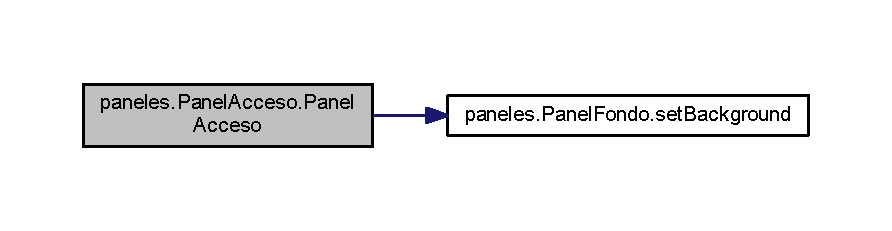
\includegraphics[width=350pt]{classpaneles_1_1_panel_acceso_ab19590219a09f461529209808b8dbd25_cgraph}
\end{center}
\end{figure}


\subsection{Member Function Documentation}
\mbox{\Hypertarget{classpaneles_1_1_panel_acceso_ac978a2c0e1aef22aa66b19abe354b02b}\label{classpaneles_1_1_panel_acceso_ac978a2c0e1aef22aa66b19abe354b02b}} 
\index{paneles\+::\+Panel\+Acceso@{paneles\+::\+Panel\+Acceso}!get\+Panel@{get\+Panel}}
\index{get\+Panel@{get\+Panel}!paneles\+::\+Panel\+Acceso@{paneles\+::\+Panel\+Acceso}}
\subsubsection{\texorpdfstring{get\+Panel()}{getPanel()}}
{\footnotesize\ttfamily J\+Panel paneles.\+Panel\+Acceso.\+get\+Panel (\begin{DoxyParamCaption}{ }\end{DoxyParamCaption})}



Definition at line 150 of file Panel\+Acceso.\+java.

\mbox{\Hypertarget{classpaneles_1_1_panel_acceso_acff0ecd448fa0435276817069e088492}\label{classpaneles_1_1_panel_acceso_acff0ecd448fa0435276817069e088492}} 
\index{paneles\+::\+Panel\+Acceso@{paneles\+::\+Panel\+Acceso}!get\+Tf\+Password@{get\+Tf\+Password}}
\index{get\+Tf\+Password@{get\+Tf\+Password}!paneles\+::\+Panel\+Acceso@{paneles\+::\+Panel\+Acceso}}
\subsubsection{\texorpdfstring{get\+Tf\+Password()}{getTfPassword()}}
{\footnotesize\ttfamily J\+Password\+Field paneles.\+Panel\+Acceso.\+get\+Tf\+Password (\begin{DoxyParamCaption}{ }\end{DoxyParamCaption})}



Definition at line 158 of file Panel\+Acceso.\+java.

\mbox{\Hypertarget{classpaneles_1_1_panel_acceso_a2e9e57df2c86935dcee9830931a7d3ec}\label{classpaneles_1_1_panel_acceso_a2e9e57df2c86935dcee9830931a7d3ec}} 
\index{paneles\+::\+Panel\+Acceso@{paneles\+::\+Panel\+Acceso}!get\+Tf\+Usuario@{get\+Tf\+Usuario}}
\index{get\+Tf\+Usuario@{get\+Tf\+Usuario}!paneles\+::\+Panel\+Acceso@{paneles\+::\+Panel\+Acceso}}
\subsubsection{\texorpdfstring{get\+Tf\+Usuario()}{getTfUsuario()}}
{\footnotesize\ttfamily J\+Text\+Field paneles.\+Panel\+Acceso.\+get\+Tf\+Usuario (\begin{DoxyParamCaption}{ }\end{DoxyParamCaption})}



Definition at line 154 of file Panel\+Acceso.\+java.



The documentation for this class was generated from the following file\+:\begin{DoxyCompactItemize}
\item 
C\+:/\+Users/jonmu/\+Desktop/\+P\+O\+P\+B\+L 4/src/paneles/\mbox{\hyperlink{_panel_acceso_8java}{Panel\+Acceso.\+java}}\end{DoxyCompactItemize}

\hypertarget{classpaneles_1_1_panel_estados}{}\section{paneles.\+Panel\+Estados Class Reference}
\label{classpaneles_1_1_panel_estados}\index{paneles.\+Panel\+Estados@{paneles.\+Panel\+Estados}}


Inheritance diagram for paneles.\+Panel\+Estados\+:
% FIG 0


Collaboration diagram for paneles.\+Panel\+Estados\+:
% FIG 1
\subsection*{Public Member Functions}
\begin{DoxyCompactItemize}
\item 
\mbox{\Hypertarget{classpaneles_1_1_panel_estados_a58b73ebb992e4dd681a60d7d1d8497c2}\label{classpaneles_1_1_panel_estados_a58b73ebb992e4dd681a60d7d1d8497c2}} 
{\bfseries Panel\+Estados} (\mbox{\hyperlink{classvistas_1_1_principal}{Principal}} principal)
\item 
\mbox{\Hypertarget{classpaneles_1_1_panel_estados_ae62e5c6656177ec67c97cc2fe48d1e54}\label{classpaneles_1_1_panel_estados_ae62e5c6656177ec67c97cc2fe48d1e54}} 
Component {\bfseries crear\+Toolbar} ()
\item 
\mbox{\Hypertarget{classpaneles_1_1_panel_estados_af627b3edddac65046fd93dc774904597}\label{classpaneles_1_1_panel_estados_af627b3edddac65046fd93dc774904597}} 
Component {\bfseries crear\+Boton\+Toolbar} (String nombre\+Boton)
\item 
\mbox{\Hypertarget{classpaneles_1_1_panel_estados_a8f949a32d4a35371a2f2b37a66ede21c}\label{classpaneles_1_1_panel_estados_a8f949a32d4a35371a2f2b37a66ede21c}} 
J\+Panel {\bfseries get\+Panel} ()
\item 
\mbox{\Hypertarget{classpaneles_1_1_panel_estados_a317a78c32717a2c06cbb82f990e411ff}\label{classpaneles_1_1_panel_estados_a317a78c32717a2c06cbb82f990e411ff}} 
void {\bfseries table\+Changed} (Table\+Model\+Event e)
\item 
\mbox{\Hypertarget{classpaneles_1_1_panel_estados_a2042bfd835f4ceea6a1e055cc388add5}\label{classpaneles_1_1_panel_estados_a2042bfd835f4ceea6a1e055cc388add5}} 
void {\bfseries mouse\+Clicked} (Mouse\+Event e)
\item 
\mbox{\Hypertarget{classpaneles_1_1_panel_estados_a4bb90c78460058ff38dd8d70d4bc4db8}\label{classpaneles_1_1_panel_estados_a4bb90c78460058ff38dd8d70d4bc4db8}} 
void {\bfseries mouse\+Pressed} (Mouse\+Event e)
\item 
\mbox{\Hypertarget{classpaneles_1_1_panel_estados_a1a35a3b4c3144a440153fccd3da616fd}\label{classpaneles_1_1_panel_estados_a1a35a3b4c3144a440153fccd3da616fd}} 
void {\bfseries mouse\+Released} (Mouse\+Event e)
\item 
\mbox{\Hypertarget{classpaneles_1_1_panel_estados_a6636a93391632082ad778cea6d6189b7}\label{classpaneles_1_1_panel_estados_a6636a93391632082ad778cea6d6189b7}} 
void {\bfseries mouse\+Entered} (Mouse\+Event e)
\item 
\mbox{\Hypertarget{classpaneles_1_1_panel_estados_a1e46995f291f6fbbb7686c141a24d4da}\label{classpaneles_1_1_panel_estados_a1e46995f291f6fbbb7686c141a24d4da}} 
void {\bfseries mouse\+Exited} (Mouse\+Event e)
\end{DoxyCompactItemize}


The documentation for this class was generated from the following file\+:\begin{DoxyCompactItemize}
\item 
C\+:/\+Users/jonmu/\+Desktop/\+P\+O\+P\+B\+L 4/src/paneles/Panel\+Estados.\+java\end{DoxyCompactItemize}

\hypertarget{classpaneles_1_1_panel_fondo}{}\section{paneles.\+Panel\+Fondo Class Reference}
\label{classpaneles_1_1_panel_fondo}\index{paneles.\+Panel\+Fondo@{paneles.\+Panel\+Fondo}}


Inheritance diagram for paneles.\+Panel\+Fondo\+:
\nopagebreak
\begin{figure}[H]
\begin{center}
\leavevmode
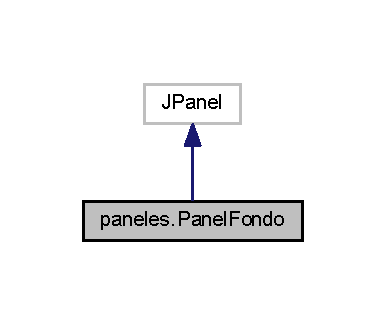
\includegraphics[width=185pt]{classpaneles_1_1_panel_fondo__inherit__graph}
\end{center}
\end{figure}


Collaboration diagram for paneles.\+Panel\+Fondo\+:
\nopagebreak
\begin{figure}[H]
\begin{center}
\leavevmode
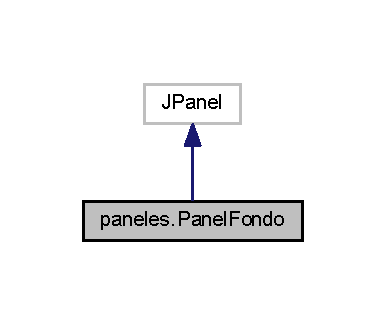
\includegraphics[width=185pt]{classpaneles_1_1_panel_fondo__coll__graph}
\end{center}
\end{figure}
\subsection*{Public Member Functions}
\begin{DoxyCompactItemize}
\item 
\mbox{\hyperlink{classpaneles_1_1_panel_fondo_a64adb64396f808c54e8d9c5383a45531}{Panel\+Fondo}} ()
\item 
void \mbox{\hyperlink{classpaneles_1_1_panel_fondo_aeaeb3ac61110f0e637b22afc5111e9d7}{paint\+Component}} (Graphics g)
\item 
void \mbox{\hyperlink{classpaneles_1_1_panel_fondo_ae95bde361bef113903c6fa6b1b65acf2}{set\+Background}} (String image\+Path)
\end{DoxyCompactItemize}


\subsection{Detailed Description}


Definition at line 10 of file Panel\+Fondo.\+java.



\subsection{Constructor \& Destructor Documentation}
\mbox{\Hypertarget{classpaneles_1_1_panel_fondo_a64adb64396f808c54e8d9c5383a45531}\label{classpaneles_1_1_panel_fondo_a64adb64396f808c54e8d9c5383a45531}} 
\index{paneles\+::\+Panel\+Fondo@{paneles\+::\+Panel\+Fondo}!Panel\+Fondo@{Panel\+Fondo}}
\index{Panel\+Fondo@{Panel\+Fondo}!paneles\+::\+Panel\+Fondo@{paneles\+::\+Panel\+Fondo}}
\subsubsection{\texorpdfstring{Panel\+Fondo()}{PanelFondo()}}
{\footnotesize\ttfamily paneles.\+Panel\+Fondo.\+Panel\+Fondo (\begin{DoxyParamCaption}{ }\end{DoxyParamCaption})}



Definition at line 14 of file Panel\+Fondo.\+java.



\subsection{Member Function Documentation}
\mbox{\Hypertarget{classpaneles_1_1_panel_fondo_aeaeb3ac61110f0e637b22afc5111e9d7}\label{classpaneles_1_1_panel_fondo_aeaeb3ac61110f0e637b22afc5111e9d7}} 
\index{paneles\+::\+Panel\+Fondo@{paneles\+::\+Panel\+Fondo}!paint\+Component@{paint\+Component}}
\index{paint\+Component@{paint\+Component}!paneles\+::\+Panel\+Fondo@{paneles\+::\+Panel\+Fondo}}
\subsubsection{\texorpdfstring{paint\+Component()}{paintComponent()}}
{\footnotesize\ttfamily void paneles.\+Panel\+Fondo.\+paint\+Component (\begin{DoxyParamCaption}\item[{Graphics}]{g }\end{DoxyParamCaption})}



Definition at line 17 of file Panel\+Fondo.\+java.

\mbox{\Hypertarget{classpaneles_1_1_panel_fondo_ae95bde361bef113903c6fa6b1b65acf2}\label{classpaneles_1_1_panel_fondo_ae95bde361bef113903c6fa6b1b65acf2}} 
\index{paneles\+::\+Panel\+Fondo@{paneles\+::\+Panel\+Fondo}!set\+Background@{set\+Background}}
\index{set\+Background@{set\+Background}!paneles\+::\+Panel\+Fondo@{paneles\+::\+Panel\+Fondo}}
\subsubsection{\texorpdfstring{set\+Background()}{setBackground()}}
{\footnotesize\ttfamily void paneles.\+Panel\+Fondo.\+set\+Background (\begin{DoxyParamCaption}\item[{String}]{image\+Path }\end{DoxyParamCaption})}



Definition at line 27 of file Panel\+Fondo.\+java.



The documentation for this class was generated from the following file\+:\begin{DoxyCompactItemize}
\item 
C\+:/\+Users/jonmu/\+Desktop/\+P\+O\+P\+B\+L 4/src/paneles/\mbox{\hyperlink{_panel_fondo_8java}{Panel\+Fondo.\+java}}\end{DoxyCompactItemize}

\hypertarget{classpaneles_1_1_panel_menu_admin}{}\section{paneles.\+Panel\+Menu\+Admin Class Reference}
\label{classpaneles_1_1_panel_menu_admin}\index{paneles.\+Panel\+Menu\+Admin@{paneles.\+Panel\+Menu\+Admin}}


Collaboration diagram for paneles.\+Panel\+Menu\+Admin\+:
% FIG 0
\subsection*{Public Member Functions}
\begin{DoxyCompactItemize}
\item 
\mbox{\Hypertarget{classpaneles_1_1_panel_menu_admin_ae686f35c694b90e334b64c385aa959ee}\label{classpaneles_1_1_panel_menu_admin_ae686f35c694b90e334b64c385aa959ee}} 
{\bfseries Panel\+Menu\+Admin} (\mbox{\hyperlink{classvistas_1_1_principal}{Principal}} principal)
\item 
\mbox{\Hypertarget{classpaneles_1_1_panel_menu_admin_a45a3165ede4cd4e1d926a7d07cedc8a1}\label{classpaneles_1_1_panel_menu_admin_a45a3165ede4cd4e1d926a7d07cedc8a1}} 
J\+Panel {\bfseries get\+Panel} ()
\end{DoxyCompactItemize}


The documentation for this class was generated from the following file\+:\begin{DoxyCompactItemize}
\item 
C\+:/\+Users/jonmu/\+Desktop/\+P\+O\+P\+B\+L 4/src/paneles/Panel\+Menu\+Admin.\+java\end{DoxyCompactItemize}

\hypertarget{classpaneles_1_1_panel_pedidos_admin}{}\section{paneles.\+Panel\+Pedidos\+Admin Class Reference}
\label{classpaneles_1_1_panel_pedidos_admin}\index{paneles.\+Panel\+Pedidos\+Admin@{paneles.\+Panel\+Pedidos\+Admin}}


Inheritance diagram for paneles.\+Panel\+Pedidos\+Admin\+:
\nopagebreak
\begin{figure}[H]
\begin{center}
\leavevmode
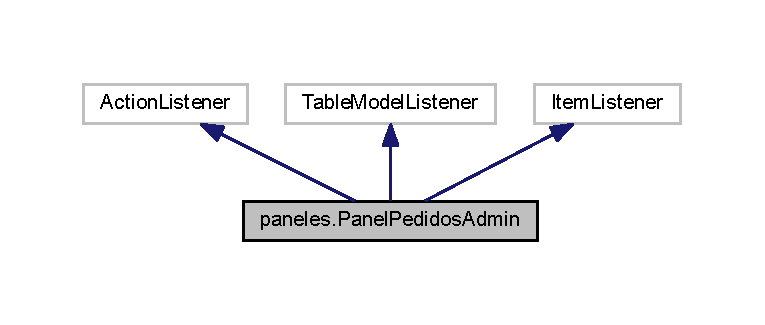
\includegraphics[width=350pt]{classpaneles_1_1_panel_pedidos_admin__inherit__graph}
\end{center}
\end{figure}


Collaboration diagram for paneles.\+Panel\+Pedidos\+Admin\+:
\nopagebreak
\begin{figure}[H]
\begin{center}
\leavevmode
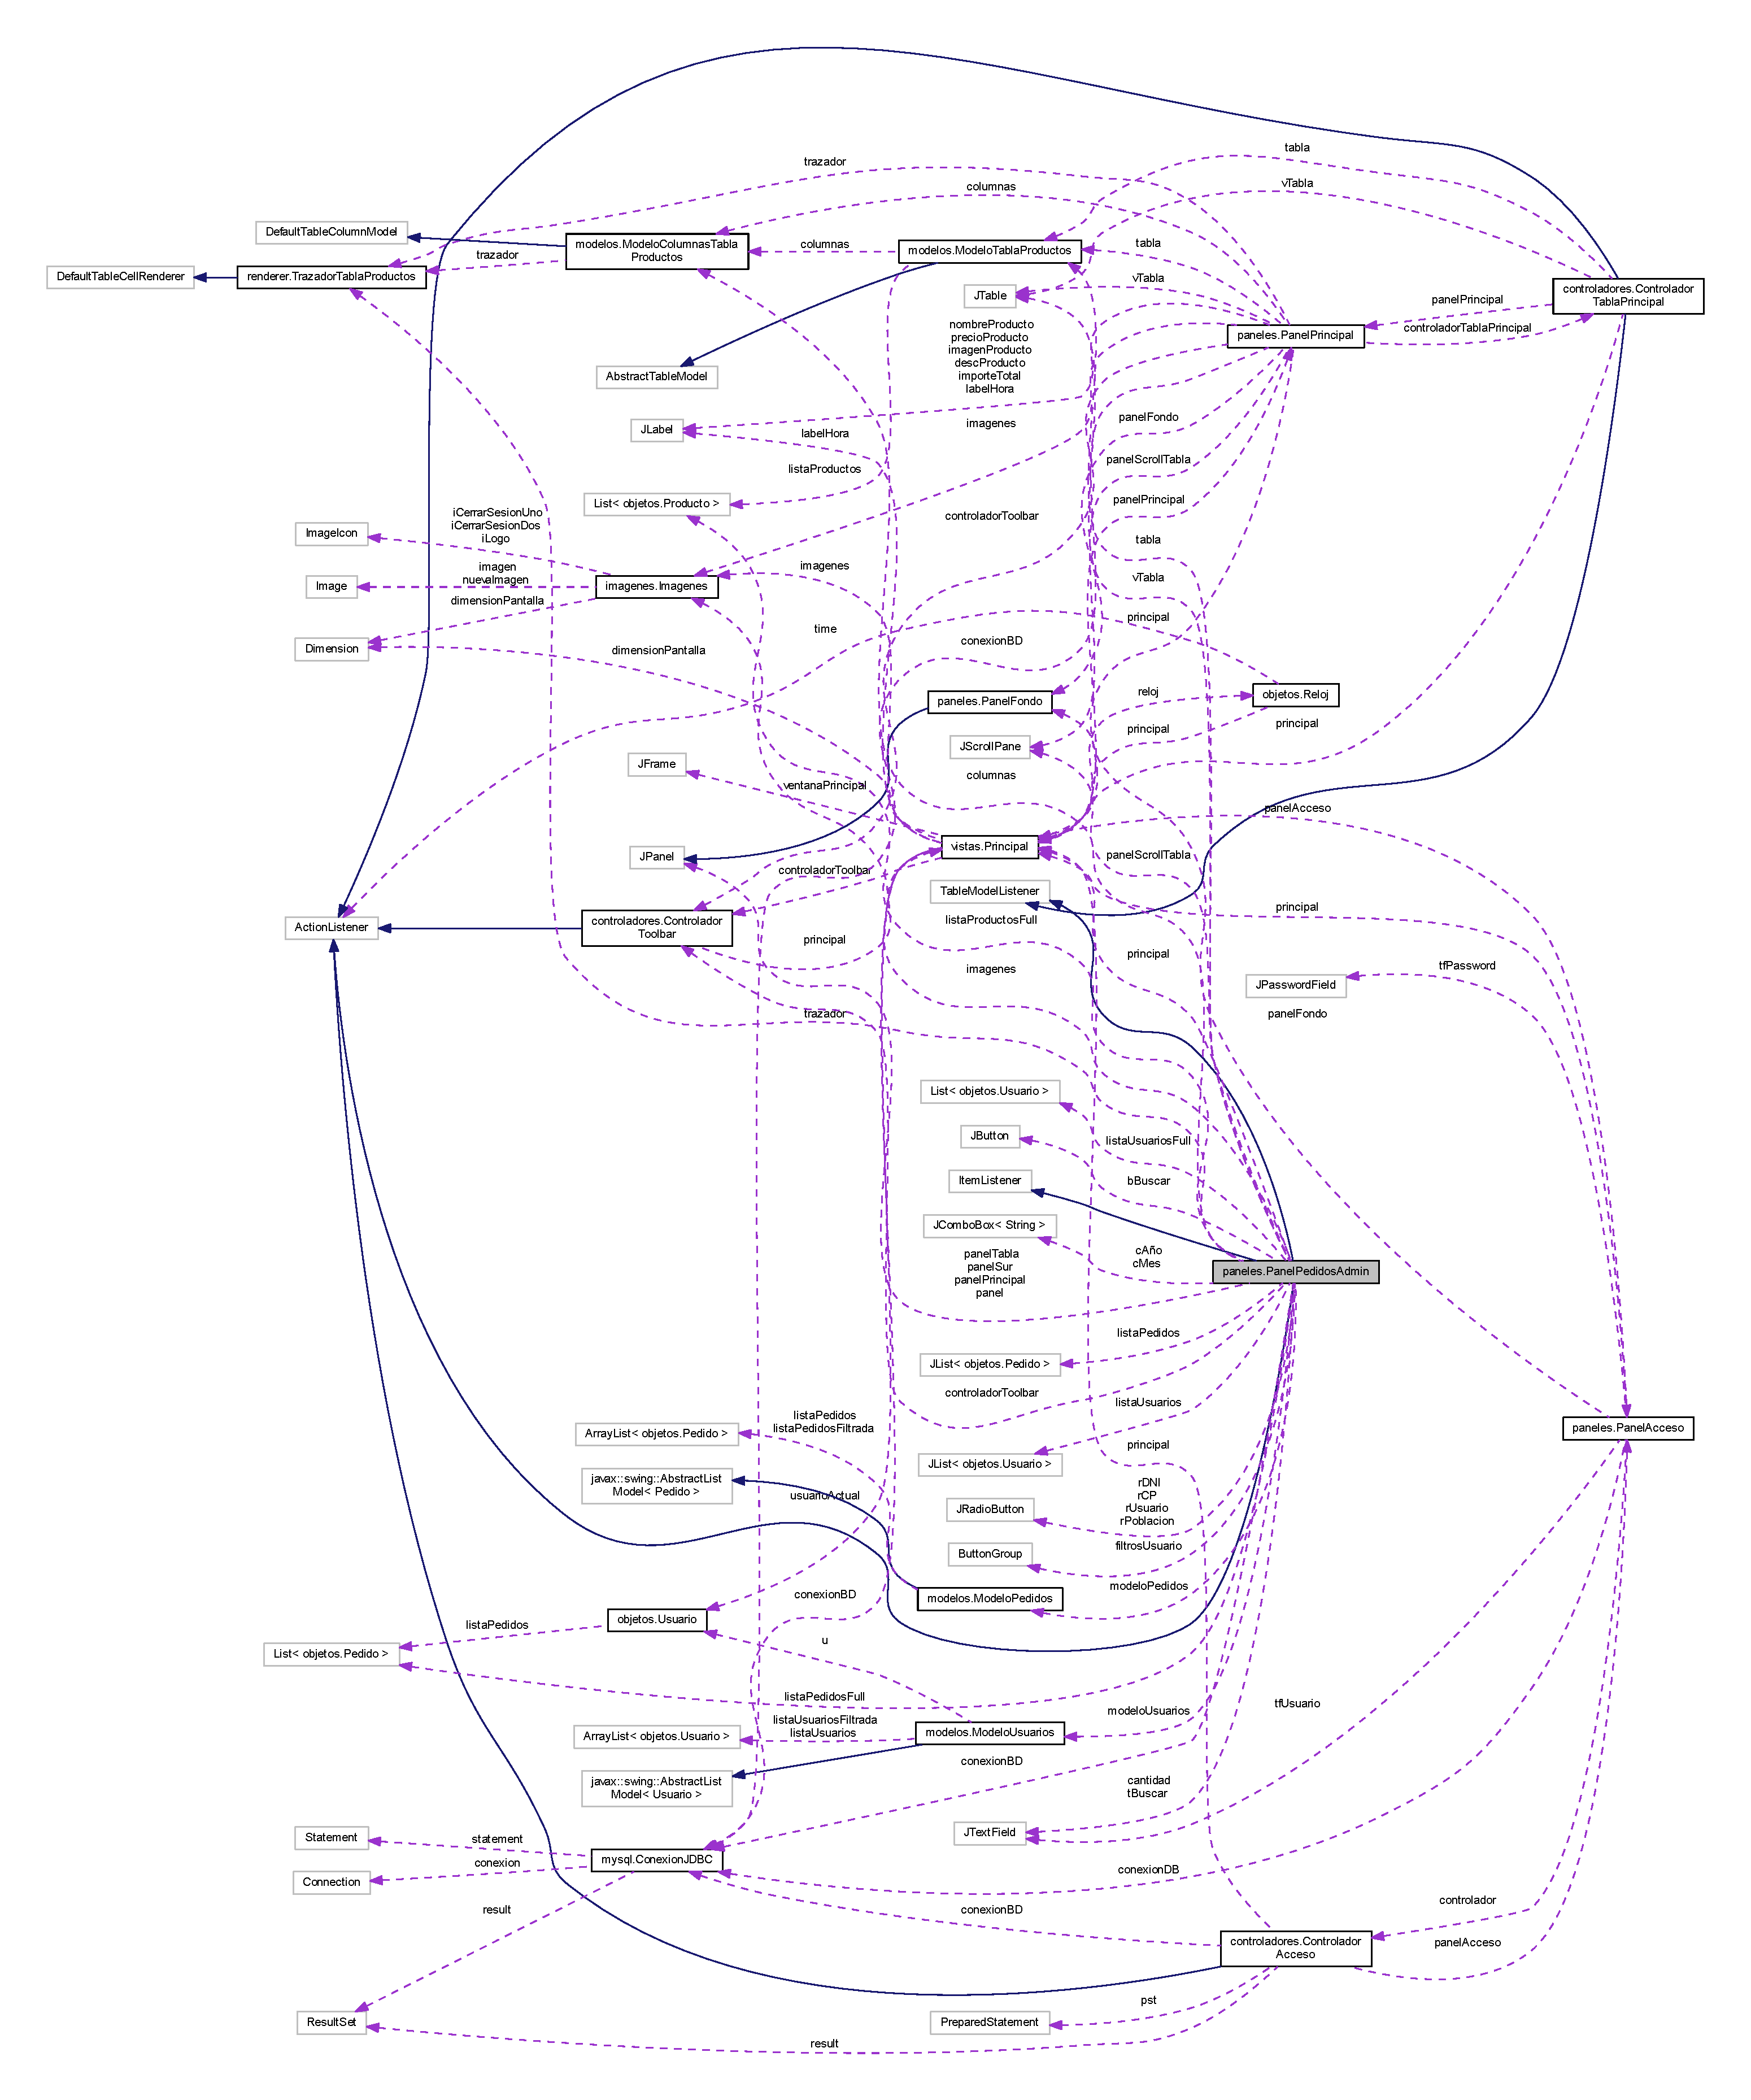
\includegraphics[width=350pt]{classpaneles_1_1_panel_pedidos_admin__coll__graph}
\end{center}
\end{figure}
\subsection*{Public Member Functions}
\begin{DoxyCompactItemize}
\item 
\mbox{\hyperlink{classpaneles_1_1_panel_pedidos_admin_abe62da27a8eab1d1ff135f2d0afd1924}{Panel\+Pedidos\+Admin}} (\mbox{\hyperlink{classmysql_1_1_conexion_j_d_b_c}{Conexion\+J\+D\+BC}} conexion\+BD, \mbox{\hyperlink{classvistas_1_1_principal}{Principal}} principal)  throws Class\+Not\+Found\+Exception, S\+Q\+L\+Exception, I\+O\+Exception 
\item 
Component \mbox{\hyperlink{classpaneles_1_1_panel_pedidos_admin_a700eb718ad003fd6132347117e6842c2}{crear\+Split\+Principal}} ()
\item 
Component \mbox{\hyperlink{classpaneles_1_1_panel_pedidos_admin_a3479b5a4aa009da3d3e99ad6ad689a57}{crear\+Toolbar}} ()
\item 
Component \mbox{\hyperlink{classpaneles_1_1_panel_pedidos_admin_aefe83135ca649c6b08d56372acada534}{crear\+Boton\+Toolbar}} (String nombre\+Boton)
\item 
List$<$ \mbox{\hyperlink{classobjetos_1_1_usuario}{Usuario}} $>$ \mbox{\hyperlink{classpaneles_1_1_panel_pedidos_admin_a3f0248c018216056a00b353d5f13f097}{crear\+Lista\+Completa}} ()  throws Class\+Not\+Found\+Exception, S\+Q\+L\+Exception 
\item 
J\+Panel \mbox{\hyperlink{classpaneles_1_1_panel_pedidos_admin_a76287d5b003f15b41fd889936a6e817e}{get\+Panel}} ()
\item 
void \mbox{\hyperlink{classpaneles_1_1_panel_pedidos_admin_aa7bdfe0ead2f6ae46989dc2f4413790e}{action\+Performed}} (Action\+Event e)
\item 
void \mbox{\hyperlink{classpaneles_1_1_panel_pedidos_admin_a484c4ce5aa6fa7f33fb62eb4b9521940}{table\+Changed}} (Table\+Model\+Event e)
\item 
void \mbox{\hyperlink{classpaneles_1_1_panel_pedidos_admin_a977e74f76b8513055d320e5b976e2143}{item\+State\+Changed}} (Item\+Event e)
\end{DoxyCompactItemize}


\subsection{Detailed Description}


Definition at line 53 of file Panel\+Pedidos\+Admin.\+java.



\subsection{Constructor \& Destructor Documentation}
\mbox{\Hypertarget{classpaneles_1_1_panel_pedidos_admin_abe62da27a8eab1d1ff135f2d0afd1924}\label{classpaneles_1_1_panel_pedidos_admin_abe62da27a8eab1d1ff135f2d0afd1924}} 
\index{paneles\+::\+Panel\+Pedidos\+Admin@{paneles\+::\+Panel\+Pedidos\+Admin}!Panel\+Pedidos\+Admin@{Panel\+Pedidos\+Admin}}
\index{Panel\+Pedidos\+Admin@{Panel\+Pedidos\+Admin}!paneles\+::\+Panel\+Pedidos\+Admin@{paneles\+::\+Panel\+Pedidos\+Admin}}
\subsubsection{\texorpdfstring{Panel\+Pedidos\+Admin()}{PanelPedidosAdmin()}}
{\footnotesize\ttfamily paneles.\+Panel\+Pedidos\+Admin.\+Panel\+Pedidos\+Admin (\begin{DoxyParamCaption}\item[{\mbox{\hyperlink{classmysql_1_1_conexion_j_d_b_c}{Conexion\+J\+D\+BC}}}]{conexion\+BD,  }\item[{\mbox{\hyperlink{classvistas_1_1_principal}{Principal}}}]{principal }\end{DoxyParamCaption}) throws Class\+Not\+Found\+Exception, S\+Q\+L\+Exception, I\+O\+Exception}



Definition at line 88 of file Panel\+Pedidos\+Admin.\+java.

Here is the call graph for this function\+:
\nopagebreak
\begin{figure}[H]
\begin{center}
\leavevmode
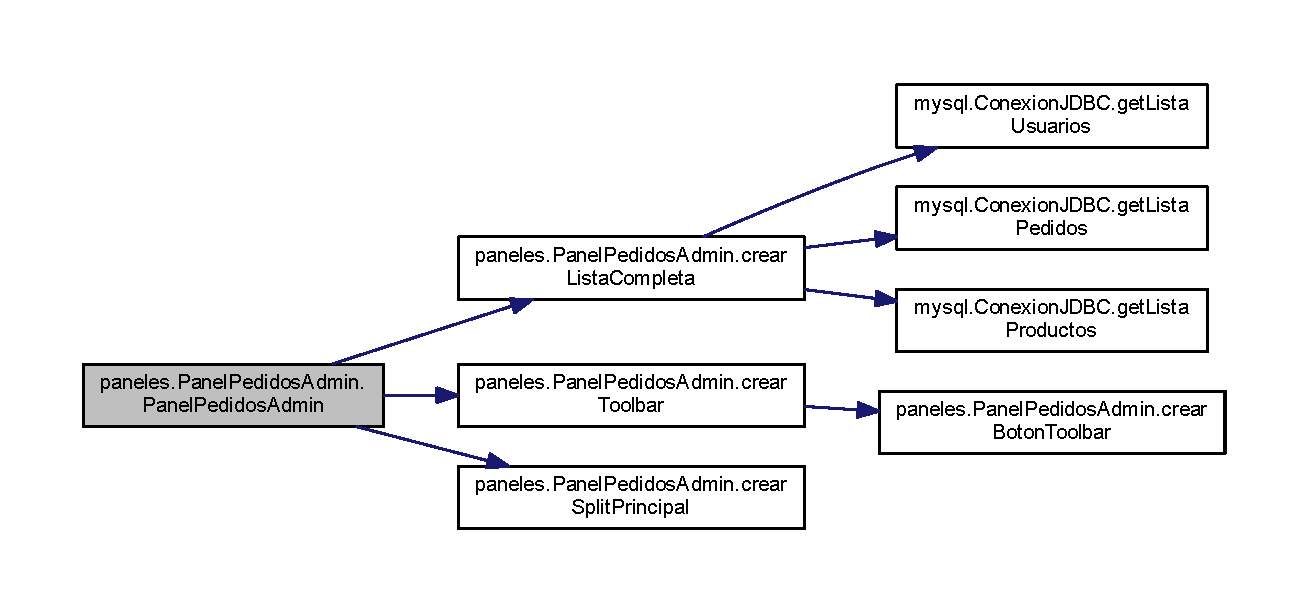
\includegraphics[width=350pt]{classpaneles_1_1_panel_pedidos_admin_abe62da27a8eab1d1ff135f2d0afd1924_cgraph}
\end{center}
\end{figure}


\subsection{Member Function Documentation}
\mbox{\Hypertarget{classpaneles_1_1_panel_pedidos_admin_aa7bdfe0ead2f6ae46989dc2f4413790e}\label{classpaneles_1_1_panel_pedidos_admin_aa7bdfe0ead2f6ae46989dc2f4413790e}} 
\index{paneles\+::\+Panel\+Pedidos\+Admin@{paneles\+::\+Panel\+Pedidos\+Admin}!action\+Performed@{action\+Performed}}
\index{action\+Performed@{action\+Performed}!paneles\+::\+Panel\+Pedidos\+Admin@{paneles\+::\+Panel\+Pedidos\+Admin}}
\subsubsection{\texorpdfstring{action\+Performed()}{actionPerformed()}}
{\footnotesize\ttfamily void paneles.\+Panel\+Pedidos\+Admin.\+action\+Performed (\begin{DoxyParamCaption}\item[{Action\+Event}]{e }\end{DoxyParamCaption})}



Definition at line 360 of file Panel\+Pedidos\+Admin.\+java.

Here is the call graph for this function\+:
\nopagebreak
\begin{figure}[H]
\begin{center}
\leavevmode
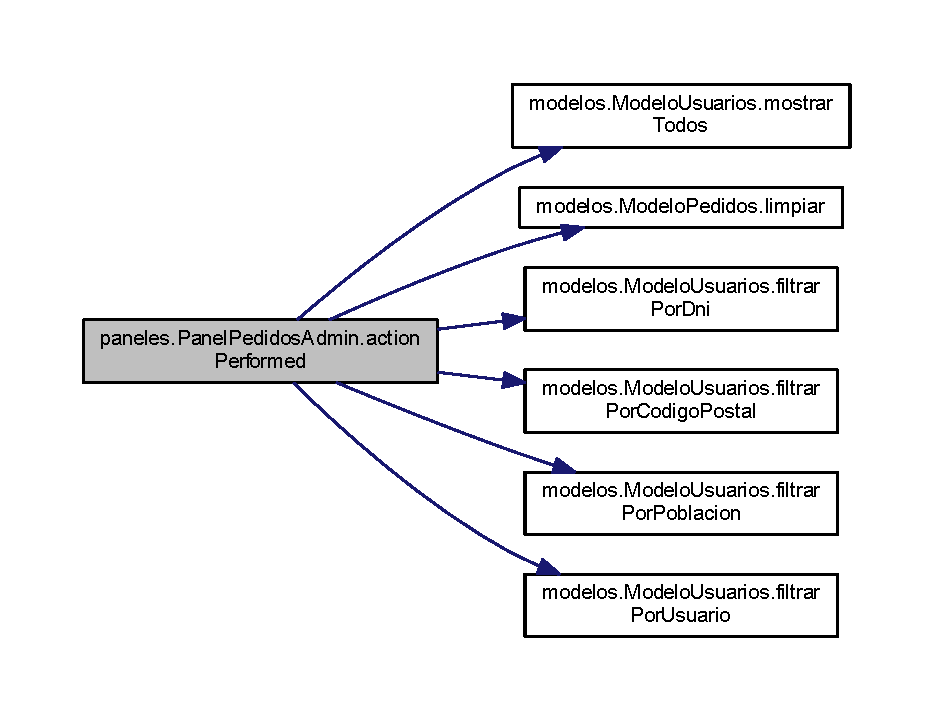
\includegraphics[width=350pt]{classpaneles_1_1_panel_pedidos_admin_aa7bdfe0ead2f6ae46989dc2f4413790e_cgraph}
\end{center}
\end{figure}
\mbox{\Hypertarget{classpaneles_1_1_panel_pedidos_admin_aefe83135ca649c6b08d56372acada534}\label{classpaneles_1_1_panel_pedidos_admin_aefe83135ca649c6b08d56372acada534}} 
\index{paneles\+::\+Panel\+Pedidos\+Admin@{paneles\+::\+Panel\+Pedidos\+Admin}!crear\+Boton\+Toolbar@{crear\+Boton\+Toolbar}}
\index{crear\+Boton\+Toolbar@{crear\+Boton\+Toolbar}!paneles\+::\+Panel\+Pedidos\+Admin@{paneles\+::\+Panel\+Pedidos\+Admin}}
\subsubsection{\texorpdfstring{crear\+Boton\+Toolbar()}{crearBotonToolbar()}}
{\footnotesize\ttfamily Component paneles.\+Panel\+Pedidos\+Admin.\+crear\+Boton\+Toolbar (\begin{DoxyParamCaption}\item[{String}]{nombre\+Boton }\end{DoxyParamCaption})}



Definition at line 131 of file Panel\+Pedidos\+Admin.\+java.

\mbox{\Hypertarget{classpaneles_1_1_panel_pedidos_admin_a3f0248c018216056a00b353d5f13f097}\label{classpaneles_1_1_panel_pedidos_admin_a3f0248c018216056a00b353d5f13f097}} 
\index{paneles\+::\+Panel\+Pedidos\+Admin@{paneles\+::\+Panel\+Pedidos\+Admin}!crear\+Lista\+Completa@{crear\+Lista\+Completa}}
\index{crear\+Lista\+Completa@{crear\+Lista\+Completa}!paneles\+::\+Panel\+Pedidos\+Admin@{paneles\+::\+Panel\+Pedidos\+Admin}}
\subsubsection{\texorpdfstring{crear\+Lista\+Completa()}{crearListaCompleta()}}
{\footnotesize\ttfamily List$<$\mbox{\hyperlink{classobjetos_1_1_usuario}{Usuario}}$>$ paneles.\+Panel\+Pedidos\+Admin.\+crear\+Lista\+Completa (\begin{DoxyParamCaption}{ }\end{DoxyParamCaption}) throws Class\+Not\+Found\+Exception, S\+Q\+L\+Exception}



Definition at line 340 of file Panel\+Pedidos\+Admin.\+java.

Here is the call graph for this function\+:
\nopagebreak
\begin{figure}[H]
\begin{center}
\leavevmode
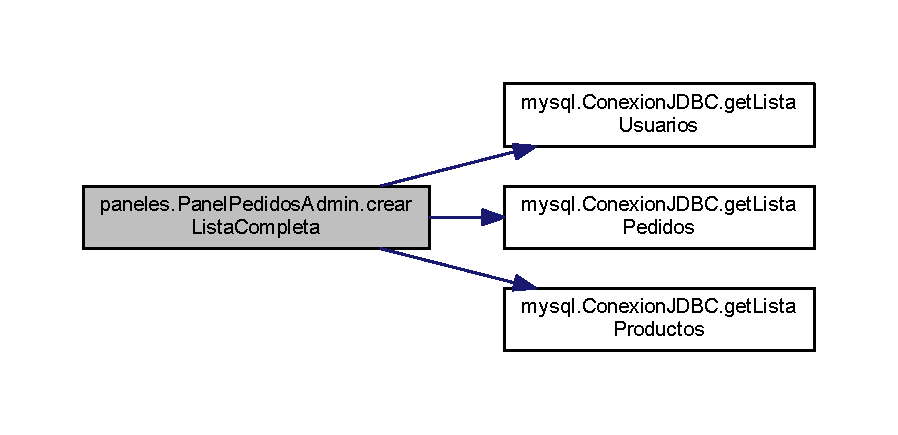
\includegraphics[width=350pt]{classpaneles_1_1_panel_pedidos_admin_a3f0248c018216056a00b353d5f13f097_cgraph}
\end{center}
\end{figure}
\mbox{\Hypertarget{classpaneles_1_1_panel_pedidos_admin_a700eb718ad003fd6132347117e6842c2}\label{classpaneles_1_1_panel_pedidos_admin_a700eb718ad003fd6132347117e6842c2}} 
\index{paneles\+::\+Panel\+Pedidos\+Admin@{paneles\+::\+Panel\+Pedidos\+Admin}!crear\+Split\+Principal@{crear\+Split\+Principal}}
\index{crear\+Split\+Principal@{crear\+Split\+Principal}!paneles\+::\+Panel\+Pedidos\+Admin@{paneles\+::\+Panel\+Pedidos\+Admin}}
\subsubsection{\texorpdfstring{crear\+Split\+Principal()}{crearSplitPrincipal()}}
{\footnotesize\ttfamily Component paneles.\+Panel\+Pedidos\+Admin.\+crear\+Split\+Principal (\begin{DoxyParamCaption}{ }\end{DoxyParamCaption})}



Definition at line 109 of file Panel\+Pedidos\+Admin.\+java.

\mbox{\Hypertarget{classpaneles_1_1_panel_pedidos_admin_a3479b5a4aa009da3d3e99ad6ad689a57}\label{classpaneles_1_1_panel_pedidos_admin_a3479b5a4aa009da3d3e99ad6ad689a57}} 
\index{paneles\+::\+Panel\+Pedidos\+Admin@{paneles\+::\+Panel\+Pedidos\+Admin}!crear\+Toolbar@{crear\+Toolbar}}
\index{crear\+Toolbar@{crear\+Toolbar}!paneles\+::\+Panel\+Pedidos\+Admin@{paneles\+::\+Panel\+Pedidos\+Admin}}
\subsubsection{\texorpdfstring{crear\+Toolbar()}{crearToolbar()}}
{\footnotesize\ttfamily Component paneles.\+Panel\+Pedidos\+Admin.\+crear\+Toolbar (\begin{DoxyParamCaption}{ }\end{DoxyParamCaption})}



Definition at line 119 of file Panel\+Pedidos\+Admin.\+java.

Here is the call graph for this function\+:
\nopagebreak
\begin{figure}[H]
\begin{center}
\leavevmode
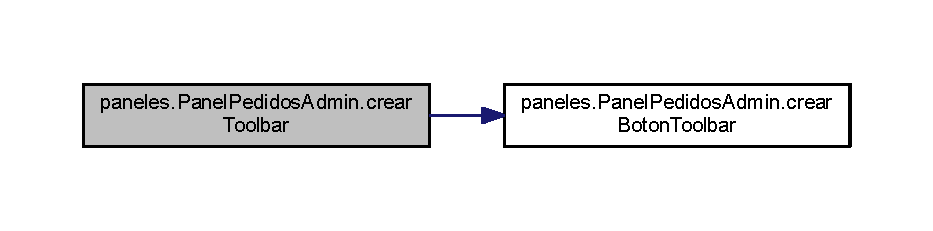
\includegraphics[width=350pt]{classpaneles_1_1_panel_pedidos_admin_a3479b5a4aa009da3d3e99ad6ad689a57_cgraph}
\end{center}
\end{figure}
\mbox{\Hypertarget{classpaneles_1_1_panel_pedidos_admin_a76287d5b003f15b41fd889936a6e817e}\label{classpaneles_1_1_panel_pedidos_admin_a76287d5b003f15b41fd889936a6e817e}} 
\index{paneles\+::\+Panel\+Pedidos\+Admin@{paneles\+::\+Panel\+Pedidos\+Admin}!get\+Panel@{get\+Panel}}
\index{get\+Panel@{get\+Panel}!paneles\+::\+Panel\+Pedidos\+Admin@{paneles\+::\+Panel\+Pedidos\+Admin}}
\subsubsection{\texorpdfstring{get\+Panel()}{getPanel()}}
{\footnotesize\ttfamily J\+Panel paneles.\+Panel\+Pedidos\+Admin.\+get\+Panel (\begin{DoxyParamCaption}{ }\end{DoxyParamCaption})}



Definition at line 355 of file Panel\+Pedidos\+Admin.\+java.

\mbox{\Hypertarget{classpaneles_1_1_panel_pedidos_admin_a977e74f76b8513055d320e5b976e2143}\label{classpaneles_1_1_panel_pedidos_admin_a977e74f76b8513055d320e5b976e2143}} 
\index{paneles\+::\+Panel\+Pedidos\+Admin@{paneles\+::\+Panel\+Pedidos\+Admin}!item\+State\+Changed@{item\+State\+Changed}}
\index{item\+State\+Changed@{item\+State\+Changed}!paneles\+::\+Panel\+Pedidos\+Admin@{paneles\+::\+Panel\+Pedidos\+Admin}}
\subsubsection{\texorpdfstring{item\+State\+Changed()}{itemStateChanged()}}
{\footnotesize\ttfamily void paneles.\+Panel\+Pedidos\+Admin.\+item\+State\+Changed (\begin{DoxyParamCaption}\item[{Item\+Event}]{e }\end{DoxyParamCaption})}



Definition at line 390 of file Panel\+Pedidos\+Admin.\+java.

Here is the call graph for this function\+:
\nopagebreak
\begin{figure}[H]
\begin{center}
\leavevmode
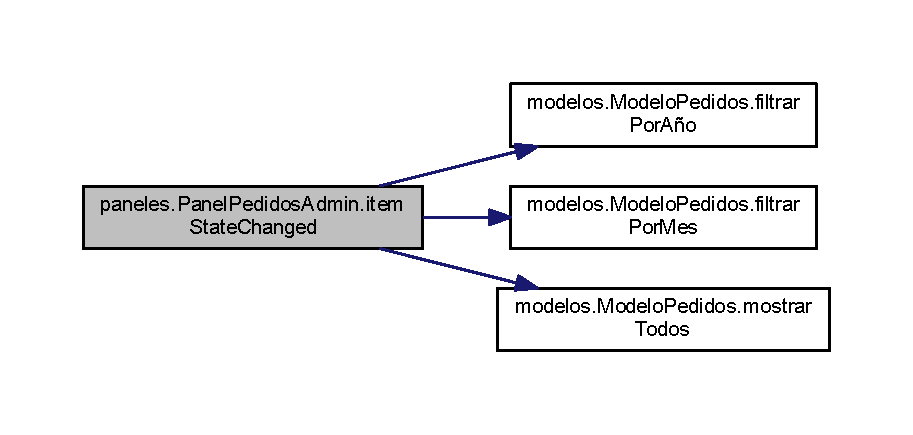
\includegraphics[width=350pt]{classpaneles_1_1_panel_pedidos_admin_a977e74f76b8513055d320e5b976e2143_cgraph}
\end{center}
\end{figure}
\mbox{\Hypertarget{classpaneles_1_1_panel_pedidos_admin_a484c4ce5aa6fa7f33fb62eb4b9521940}\label{classpaneles_1_1_panel_pedidos_admin_a484c4ce5aa6fa7f33fb62eb4b9521940}} 
\index{paneles\+::\+Panel\+Pedidos\+Admin@{paneles\+::\+Panel\+Pedidos\+Admin}!table\+Changed@{table\+Changed}}
\index{table\+Changed@{table\+Changed}!paneles\+::\+Panel\+Pedidos\+Admin@{paneles\+::\+Panel\+Pedidos\+Admin}}
\subsubsection{\texorpdfstring{table\+Changed()}{tableChanged()}}
{\footnotesize\ttfamily void paneles.\+Panel\+Pedidos\+Admin.\+table\+Changed (\begin{DoxyParamCaption}\item[{Table\+Model\+Event}]{e }\end{DoxyParamCaption})}



Definition at line 385 of file Panel\+Pedidos\+Admin.\+java.



The documentation for this class was generated from the following file\+:\begin{DoxyCompactItemize}
\item 
C\+:/\+Users/jonmu/\+Desktop/\+P\+O\+P\+B\+L 4/src/paneles/\mbox{\hyperlink{_panel_pedidos_admin_8java}{Panel\+Pedidos\+Admin.\+java}}\end{DoxyCompactItemize}

\hypertarget{classpaneles_1_1_panel_principal}{}\section{paneles.\+Panel\+Principal Class Reference}
\label{classpaneles_1_1_panel_principal}\index{paneles.\+Panel\+Principal@{paneles.\+Panel\+Principal}}


Collaboration diagram for paneles.\+Panel\+Principal\+:\nopagebreak
\begin{figure}[H]
\begin{center}
\leavevmode
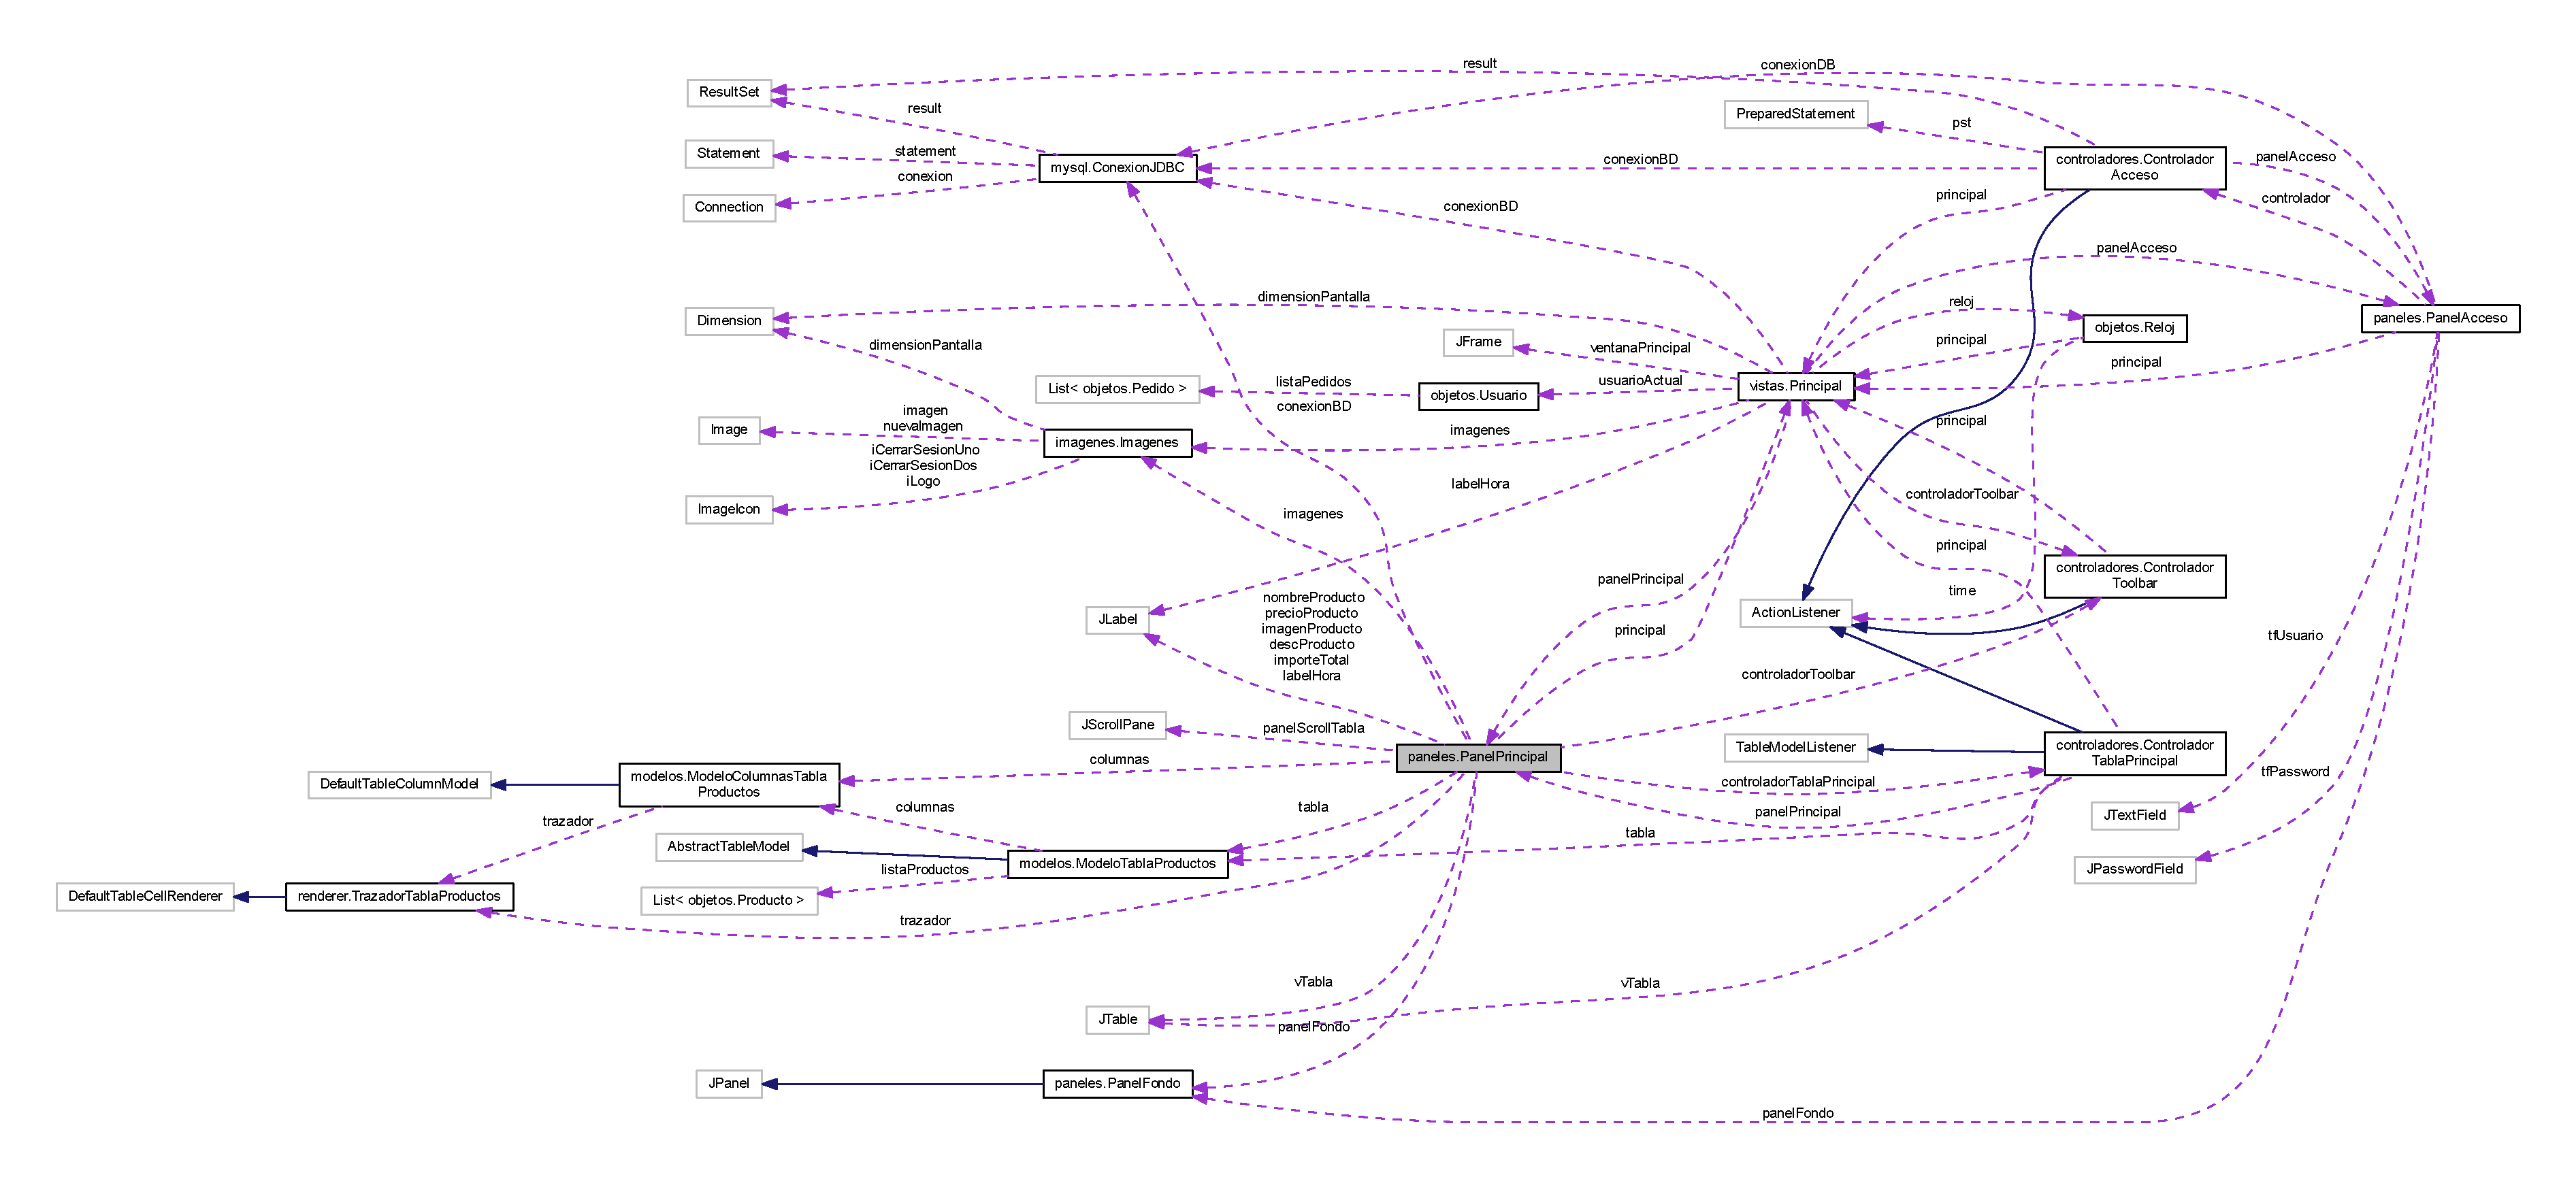
\includegraphics[width=350pt]{classpaneles_1_1_panel_principal__coll__graph}
\end{center}
\end{figure}
\subsection*{Public Member Functions}
\begin{DoxyCompactItemize}
\item 
\mbox{\hyperlink{classpaneles_1_1_panel_principal_a8f8bc1a008744e424eec12eae5e0a745}{Panel\+Principal}} (\mbox{\hyperlink{classvistas_1_1_principal}{Principal}} principal, \mbox{\hyperlink{classcontroladores_1_1_controlador_toolbar}{Controlador\+Toolbar}} controlador\+Toolbar, \mbox{\hyperlink{classimagenes_1_1_imagenes}{Imagenes}} imagenes, J\+Label label\+Hora, \mbox{\hyperlink{classmysql_1_1_conexion_j_d_b_c}{Conexion\+J\+D\+BC}} conexion\+BD)
\item 
void \mbox{\hyperlink{classpaneles_1_1_panel_principal_ad46c27384163d0757eadfe86cf72ee70}{almacenar\+Productos}} ()  throws Class\+Not\+Found\+Exception, S\+Q\+L\+Exception 
\item 
Component \mbox{\hyperlink{classpaneles_1_1_panel_principal_accd82709ae4701f14d1b5a4bbb8f3aae}{crear\+Toolbar}} ()
\item 
Component \mbox{\hyperlink{classpaneles_1_1_panel_principal_a45d159d89db6217a595c166bf2f0b2ea}{crear\+Boton\+Toolbar}} (String nombre\+Boton)
\item 
Component \mbox{\hyperlink{classpaneles_1_1_panel_principal_abf6e9ec8437453a751ea1a4bcc33fb87}{crear\+Split\+Principal}} ()
\item 
void \mbox{\hyperlink{classpaneles_1_1_panel_principal_aa2151461e479985277d05375c02b1022}{cambiar\+Producto}} ()
\item 
\mbox{\hyperlink{classpaneles_1_1_panel_fondo}{Panel\+Fondo}} \mbox{\hyperlink{classpaneles_1_1_panel_principal_ab8efee7c290494ba31d026c47dbbcefb}{get\+Panel\+Fondo}} ()
\item 
J\+Label \mbox{\hyperlink{classpaneles_1_1_panel_principal_a5ee2138a32b7b6bc6a0f7b3bd68f4821}{get\+Importe\+Total}} ()
\end{DoxyCompactItemize}


\subsection{Detailed Description}


Definition at line 42 of file Panel\+Principal.\+java.



\subsection{Constructor \& Destructor Documentation}
\mbox{\Hypertarget{classpaneles_1_1_panel_principal_a8f8bc1a008744e424eec12eae5e0a745}\label{classpaneles_1_1_panel_principal_a8f8bc1a008744e424eec12eae5e0a745}} 
\index{paneles\+::\+Panel\+Principal@{paneles\+::\+Panel\+Principal}!Panel\+Principal@{Panel\+Principal}}
\index{Panel\+Principal@{Panel\+Principal}!paneles\+::\+Panel\+Principal@{paneles\+::\+Panel\+Principal}}
\subsubsection{\texorpdfstring{Panel\+Principal()}{PanelPrincipal()}}
{\footnotesize\ttfamily paneles.\+Panel\+Principal.\+Panel\+Principal (\begin{DoxyParamCaption}\item[{\mbox{\hyperlink{classvistas_1_1_principal}{Principal}}}]{principal,  }\item[{\mbox{\hyperlink{classcontroladores_1_1_controlador_toolbar}{Controlador\+Toolbar}}}]{controlador\+Toolbar,  }\item[{\mbox{\hyperlink{classimagenes_1_1_imagenes}{Imagenes}}}]{imagenes,  }\item[{J\+Label}]{label\+Hora,  }\item[{\mbox{\hyperlink{classmysql_1_1_conexion_j_d_b_c}{Conexion\+J\+D\+BC}}}]{conexion\+BD }\end{DoxyParamCaption})}



Definition at line 64 of file Panel\+Principal.\+java.

Here is the call graph for this function\+:\nopagebreak
\begin{figure}[H]
\begin{center}
\leavevmode
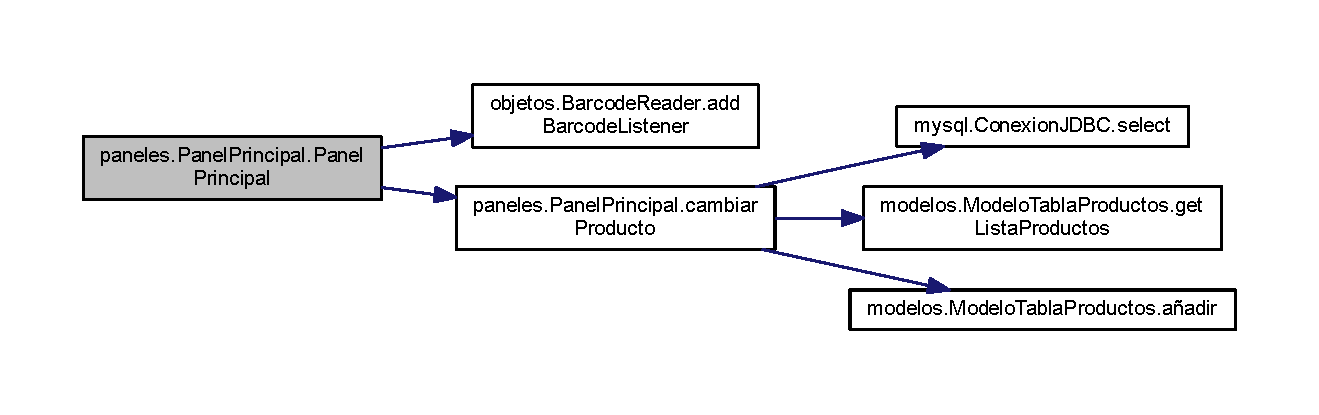
\includegraphics[width=350pt]{classpaneles_1_1_panel_principal_a8f8bc1a008744e424eec12eae5e0a745_cgraph}
\end{center}
\end{figure}


\subsection{Member Function Documentation}
\mbox{\Hypertarget{classpaneles_1_1_panel_principal_ad46c27384163d0757eadfe86cf72ee70}\label{classpaneles_1_1_panel_principal_ad46c27384163d0757eadfe86cf72ee70}} 
\index{paneles\+::\+Panel\+Principal@{paneles\+::\+Panel\+Principal}!almacenar\+Productos@{almacenar\+Productos}}
\index{almacenar\+Productos@{almacenar\+Productos}!paneles\+::\+Panel\+Principal@{paneles\+::\+Panel\+Principal}}
\subsubsection{\texorpdfstring{almacenar\+Productos()}{almacenarProductos()}}
{\footnotesize\ttfamily void paneles.\+Panel\+Principal.\+almacenar\+Productos (\begin{DoxyParamCaption}{ }\end{DoxyParamCaption}) throws Class\+Not\+Found\+Exception, S\+Q\+L\+Exception}



Definition at line 105 of file Panel\+Principal.\+java.

Here is the call graph for this function\+:\nopagebreak
\begin{figure}[H]
\begin{center}
\leavevmode
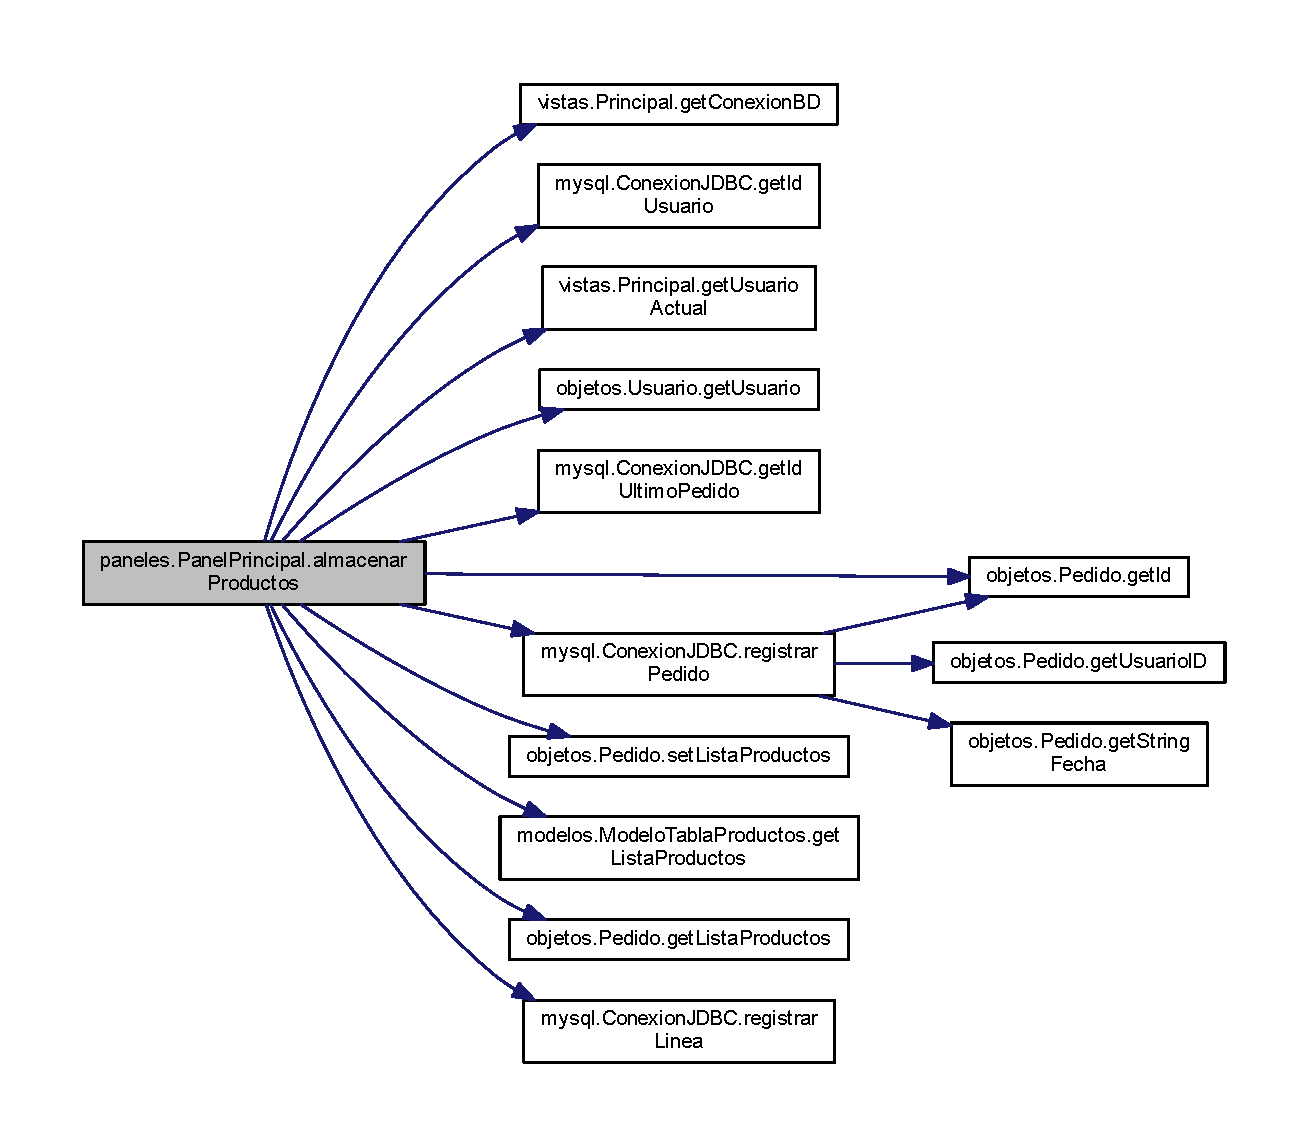
\includegraphics[width=350pt]{classpaneles_1_1_panel_principal_ad46c27384163d0757eadfe86cf72ee70_cgraph}
\end{center}
\end{figure}
\mbox{\Hypertarget{classpaneles_1_1_panel_principal_aa2151461e479985277d05375c02b1022}\label{classpaneles_1_1_panel_principal_aa2151461e479985277d05375c02b1022}} 
\index{paneles\+::\+Panel\+Principal@{paneles\+::\+Panel\+Principal}!cambiar\+Producto@{cambiar\+Producto}}
\index{cambiar\+Producto@{cambiar\+Producto}!paneles\+::\+Panel\+Principal@{paneles\+::\+Panel\+Principal}}
\subsubsection{\texorpdfstring{cambiar\+Producto()}{cambiarProducto()}}
{\footnotesize\ttfamily void paneles.\+Panel\+Principal.\+cambiar\+Producto (\begin{DoxyParamCaption}{ }\end{DoxyParamCaption})}



Definition at line 231 of file Panel\+Principal.\+java.

Here is the call graph for this function\+:\nopagebreak
\begin{figure}[H]
\begin{center}
\leavevmode
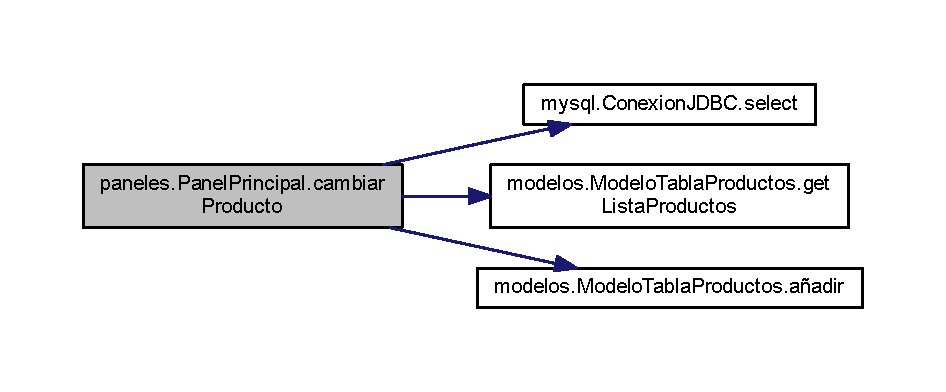
\includegraphics[width=350pt]{classpaneles_1_1_panel_principal_aa2151461e479985277d05375c02b1022_cgraph}
\end{center}
\end{figure}
\mbox{\Hypertarget{classpaneles_1_1_panel_principal_a45d159d89db6217a595c166bf2f0b2ea}\label{classpaneles_1_1_panel_principal_a45d159d89db6217a595c166bf2f0b2ea}} 
\index{paneles\+::\+Panel\+Principal@{paneles\+::\+Panel\+Principal}!crear\+Boton\+Toolbar@{crear\+Boton\+Toolbar}}
\index{crear\+Boton\+Toolbar@{crear\+Boton\+Toolbar}!paneles\+::\+Panel\+Principal@{paneles\+::\+Panel\+Principal}}
\subsubsection{\texorpdfstring{crear\+Boton\+Toolbar()}{crearBotonToolbar()}}
{\footnotesize\ttfamily Component paneles.\+Panel\+Principal.\+crear\+Boton\+Toolbar (\begin{DoxyParamCaption}\item[{String}]{nombre\+Boton }\end{DoxyParamCaption})}



Definition at line 135 of file Panel\+Principal.\+java.

\mbox{\Hypertarget{classpaneles_1_1_panel_principal_abf6e9ec8437453a751ea1a4bcc33fb87}\label{classpaneles_1_1_panel_principal_abf6e9ec8437453a751ea1a4bcc33fb87}} 
\index{paneles\+::\+Panel\+Principal@{paneles\+::\+Panel\+Principal}!crear\+Split\+Principal@{crear\+Split\+Principal}}
\index{crear\+Split\+Principal@{crear\+Split\+Principal}!paneles\+::\+Panel\+Principal@{paneles\+::\+Panel\+Principal}}
\subsubsection{\texorpdfstring{crear\+Split\+Principal()}{crearSplitPrincipal()}}
{\footnotesize\ttfamily Component paneles.\+Panel\+Principal.\+crear\+Split\+Principal (\begin{DoxyParamCaption}{ }\end{DoxyParamCaption})}



Definition at line 182 of file Panel\+Principal.\+java.

\mbox{\Hypertarget{classpaneles_1_1_panel_principal_accd82709ae4701f14d1b5a4bbb8f3aae}\label{classpaneles_1_1_panel_principal_accd82709ae4701f14d1b5a4bbb8f3aae}} 
\index{paneles\+::\+Panel\+Principal@{paneles\+::\+Panel\+Principal}!crear\+Toolbar@{crear\+Toolbar}}
\index{crear\+Toolbar@{crear\+Toolbar}!paneles\+::\+Panel\+Principal@{paneles\+::\+Panel\+Principal}}
\subsubsection{\texorpdfstring{crear\+Toolbar()}{crearToolbar()}}
{\footnotesize\ttfamily Component paneles.\+Panel\+Principal.\+crear\+Toolbar (\begin{DoxyParamCaption}{ }\end{DoxyParamCaption})}



Definition at line 122 of file Panel\+Principal.\+java.

Here is the call graph for this function\+:\nopagebreak
\begin{figure}[H]
\begin{center}
\leavevmode
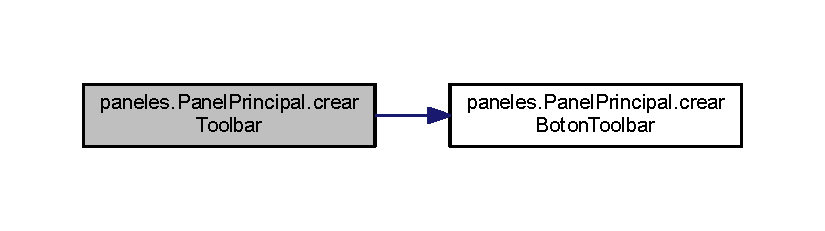
\includegraphics[width=350pt]{classpaneles_1_1_panel_principal_accd82709ae4701f14d1b5a4bbb8f3aae_cgraph}
\end{center}
\end{figure}
\mbox{\Hypertarget{classpaneles_1_1_panel_principal_a5ee2138a32b7b6bc6a0f7b3bd68f4821}\label{classpaneles_1_1_panel_principal_a5ee2138a32b7b6bc6a0f7b3bd68f4821}} 
\index{paneles\+::\+Panel\+Principal@{paneles\+::\+Panel\+Principal}!get\+Importe\+Total@{get\+Importe\+Total}}
\index{get\+Importe\+Total@{get\+Importe\+Total}!paneles\+::\+Panel\+Principal@{paneles\+::\+Panel\+Principal}}
\subsubsection{\texorpdfstring{get\+Importe\+Total()}{getImporteTotal()}}
{\footnotesize\ttfamily J\+Label paneles.\+Panel\+Principal.\+get\+Importe\+Total (\begin{DoxyParamCaption}{ }\end{DoxyParamCaption})}



Definition at line 360 of file Panel\+Principal.\+java.

\mbox{\Hypertarget{classpaneles_1_1_panel_principal_ab8efee7c290494ba31d026c47dbbcefb}\label{classpaneles_1_1_panel_principal_ab8efee7c290494ba31d026c47dbbcefb}} 
\index{paneles\+::\+Panel\+Principal@{paneles\+::\+Panel\+Principal}!get\+Panel\+Fondo@{get\+Panel\+Fondo}}
\index{get\+Panel\+Fondo@{get\+Panel\+Fondo}!paneles\+::\+Panel\+Principal@{paneles\+::\+Panel\+Principal}}
\subsubsection{\texorpdfstring{get\+Panel\+Fondo()}{getPanelFondo()}}
{\footnotesize\ttfamily \mbox{\hyperlink{classpaneles_1_1_panel_fondo}{Panel\+Fondo}} paneles.\+Panel\+Principal.\+get\+Panel\+Fondo (\begin{DoxyParamCaption}{ }\end{DoxyParamCaption})}



Definition at line 356 of file Panel\+Principal.\+java.



The documentation for this class was generated from the following file\+:\begin{DoxyCompactItemize}
\item 
C\+:/\+Users/jonmu/\+Desktop/\+P\+O\+P\+B\+L 4/src/paneles/\mbox{\hyperlink{_panel_principal_8java}{Panel\+Principal.\+java}}\end{DoxyCompactItemize}

\hypertarget{classobjetos_1_1_pedido}{}\section{objetos.\+Pedido Class Reference}
\label{classobjetos_1_1_pedido}\index{objetos.\+Pedido@{objetos.\+Pedido}}


Collaboration diagram for objetos.\+Pedido\+:
% FIG 0
\subsection*{Public Member Functions}
\begin{DoxyCompactItemize}
\item 
\mbox{\Hypertarget{classobjetos_1_1_pedido_a2f4d8a34c054b61efca09e21891dc119}\label{classobjetos_1_1_pedido_a2f4d8a34c054b61efca09e21891dc119}} 
{\bfseries Pedido} (int id, int usuario\+ID, String fecha)
\item 
\mbox{\Hypertarget{classobjetos_1_1_pedido_ac1b1b41df8f346ef077017deccf269b5}\label{classobjetos_1_1_pedido_ac1b1b41df8f346ef077017deccf269b5}} 
void {\bfseries agregar\+Producto} (\mbox{\hyperlink{classobjetos_1_1_producto}{Producto}} p)
\item 
\mbox{\Hypertarget{classobjetos_1_1_pedido_ad9981fc190fd02fbf4f9c44811fc2102}\label{classobjetos_1_1_pedido_ad9981fc190fd02fbf4f9c44811fc2102}} 
String \mbox{[}$\,$\mbox{]} {\bfseries get\+Fecha} ()
\item 
\mbox{\Hypertarget{classobjetos_1_1_pedido_a9e4f2c0942939a0defdea21140e85e94}\label{classobjetos_1_1_pedido_a9e4f2c0942939a0defdea21140e85e94}} 
List$<$ \mbox{\hyperlink{classobjetos_1_1_producto}{Producto}} $>$ {\bfseries get\+Lista\+Productos} ()
\item 
\mbox{\Hypertarget{classobjetos_1_1_pedido_af2c6fe4c929f1fce6443e3ffcb2c0a45}\label{classobjetos_1_1_pedido_af2c6fe4c929f1fce6443e3ffcb2c0a45}} 
String {\bfseries get\+String\+Fecha} ()
\item 
\mbox{\Hypertarget{classobjetos_1_1_pedido_afed5e1d427d944ead970861ef07be474}\label{classobjetos_1_1_pedido_afed5e1d427d944ead970861ef07be474}} 
int {\bfseries get\+Usuario\+ID} ()
\item 
\mbox{\Hypertarget{classobjetos_1_1_pedido_a642984750b50555899811e39208729b4}\label{classobjetos_1_1_pedido_a642984750b50555899811e39208729b4}} 
void {\bfseries set\+Lista\+Productos} (List$<$ \mbox{\hyperlink{classobjetos_1_1_producto}{Producto}} $>$ lista\+Productos)
\item 
\mbox{\Hypertarget{classobjetos_1_1_pedido_a2cedae9fd179897d4d7e83b655d6fa58}\label{classobjetos_1_1_pedido_a2cedae9fd179897d4d7e83b655d6fa58}} 
int {\bfseries get\+Id} ()
\item 
\mbox{\Hypertarget{classobjetos_1_1_pedido_a2db5b46450987a7f2fb289e19cf593ac}\label{classobjetos_1_1_pedido_a2db5b46450987a7f2fb289e19cf593ac}} 
String {\bfseries to\+String} ()
\end{DoxyCompactItemize}


The documentation for this class was generated from the following file\+:\begin{DoxyCompactItemize}
\item 
C\+:/\+Users/jonmu/\+Desktop/\+P\+O\+P\+B\+L 4/src/objetos/Pedido.\+java\end{DoxyCompactItemize}

\hypertarget{classvistas_1_1_principal}{}\section{vistas.\+Principal Class Reference}
\label{classvistas_1_1_principal}\index{vistas.\+Principal@{vistas.\+Principal}}


Collaboration diagram for vistas.\+Principal\+:
\nopagebreak
\begin{figure}[H]
\begin{center}
\leavevmode
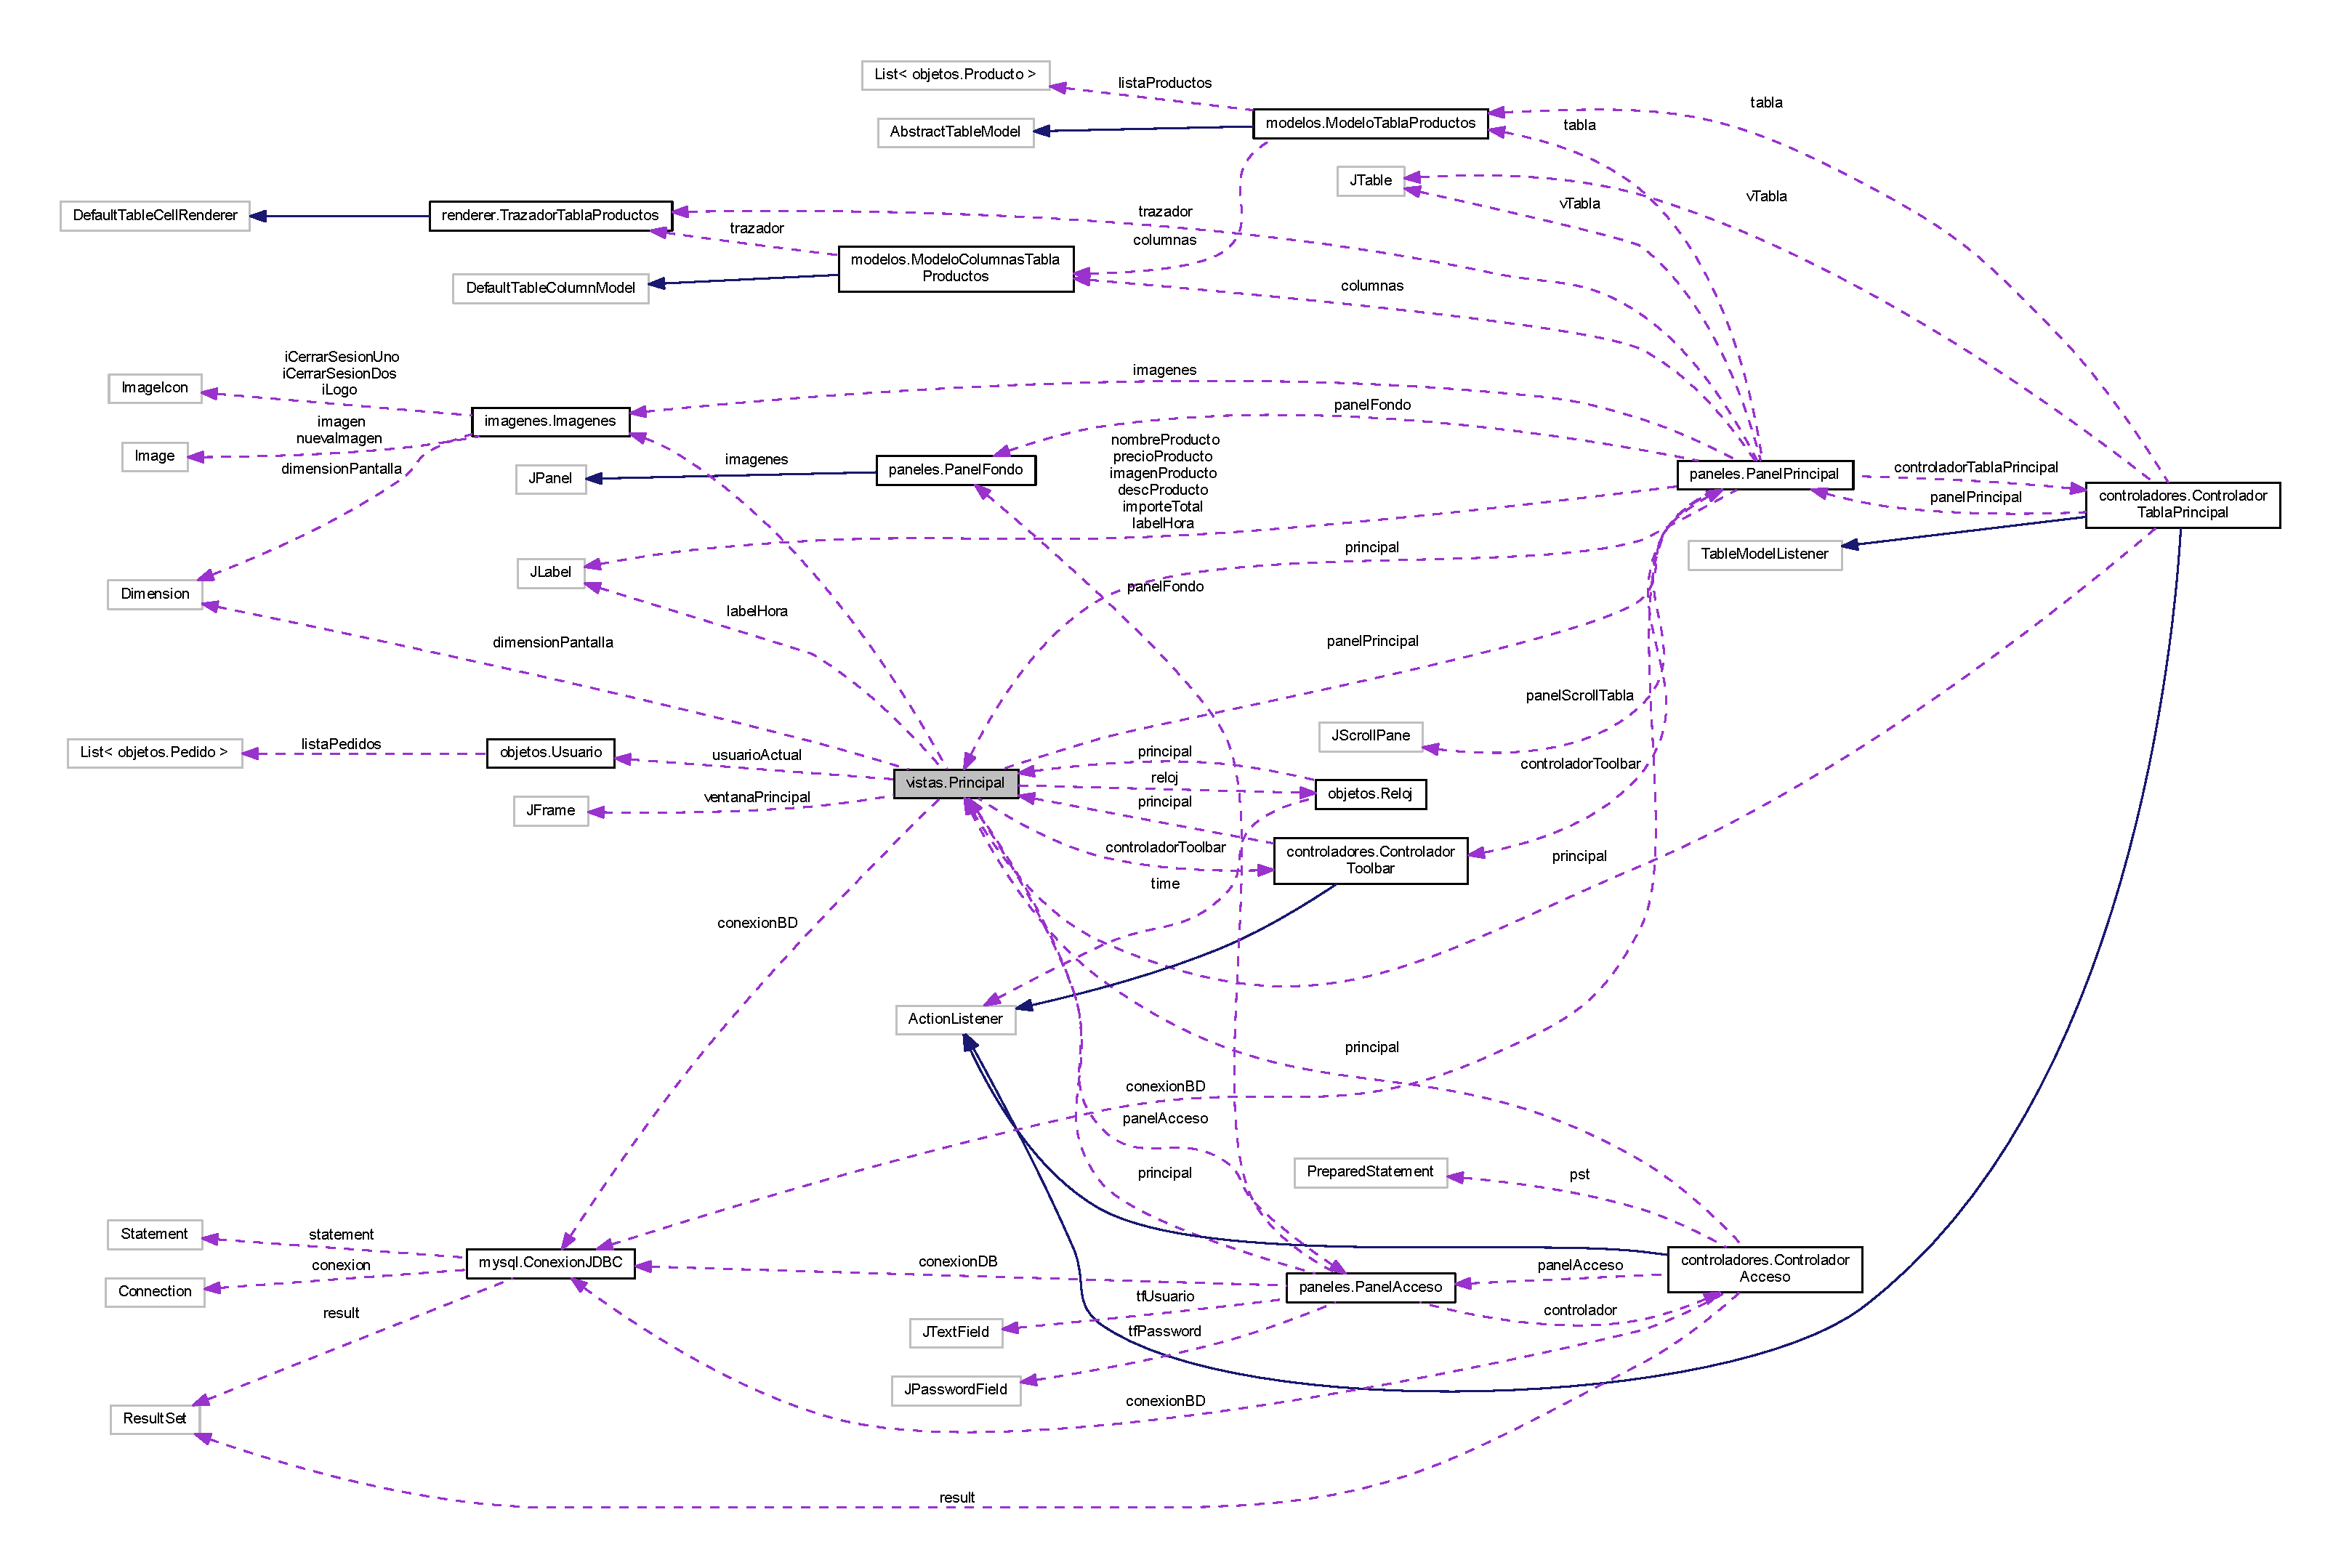
\includegraphics[width=350pt]{classvistas_1_1_principal__coll__graph}
\end{center}
\end{figure}
\subsection*{Public Member Functions}
\begin{DoxyCompactItemize}
\item 
\mbox{\hyperlink{classvistas_1_1_principal_acf014fac1f15c33d980e722fe1e6d58f}{Principal}} ()
\item 
void \mbox{\hyperlink{classvistas_1_1_principal_a0f01204c3cdf3b88718a5f2c6a6d9ac9}{cambiar\+Panel}} (J\+Panel panel)
\item 
void \mbox{\hyperlink{classvistas_1_1_principal_aa6783bab03cc60f1bf401d4c16293318}{cambiar\+Panel\+Compra}} ()
\item 
void \mbox{\hyperlink{classvistas_1_1_principal_a0823d729a42c384bf4afd30b60a3e468}{cambiar\+Panel\+Acceso}} ()
\item 
\mbox{\hyperlink{classpaneles_1_1_panel_principal}{Panel\+Principal}} \mbox{\hyperlink{classvistas_1_1_principal_a546a7dca6785535d3f48f5a7b43c20a1}{get\+Panel\+Principal}} ()
\item 
J\+Frame \mbox{\hyperlink{classvistas_1_1_principal_afc2c81827c88c9c2494b3345264e747d}{get\+Ventana\+Principal}} ()
\item 
J\+Label \mbox{\hyperlink{classvistas_1_1_principal_a95e7bccba557226e9e56211a58a2e03c}{get\+Label\+Hora}} ()
\item 
\mbox{\hyperlink{classobjetos_1_1_usuario}{Usuario}} \mbox{\hyperlink{classvistas_1_1_principal_af7ea8d6ba599873466968add34233be0}{get\+Usuario\+Actual}} ()
\item 
void \mbox{\hyperlink{classvistas_1_1_principal_a6f45e56ee7c99715b798ff202bd57d7e}{set\+Usuario\+Actual}} (\mbox{\hyperlink{classobjetos_1_1_usuario}{Usuario}} usuario\+Actual)
\item 
\mbox{\hyperlink{classmysql_1_1_conexion_j_d_b_c}{Conexion\+J\+D\+BC}} \mbox{\hyperlink{classvistas_1_1_principal_ad7379276c979124d4386d01439f24b42}{get\+Conexion\+BD}} ()
\end{DoxyCompactItemize}
\subsection*{Static Public Member Functions}
\begin{DoxyCompactItemize}
\item 
static void \mbox{\hyperlink{classvistas_1_1_principal_a626dbf26bfdd3a03a2c1c99e34d25b6c}{main}} (String\mbox{[}$\,$\mbox{]} args)
\end{DoxyCompactItemize}


\subsection{Detailed Description}


Definition at line 29 of file Principal.\+java.



\subsection{Constructor \& Destructor Documentation}
\mbox{\Hypertarget{classvistas_1_1_principal_acf014fac1f15c33d980e722fe1e6d58f}\label{classvistas_1_1_principal_acf014fac1f15c33d980e722fe1e6d58f}} 
\index{vistas\+::\+Principal@{vistas\+::\+Principal}!Principal@{Principal}}
\index{Principal@{Principal}!vistas\+::\+Principal@{vistas\+::\+Principal}}
\subsubsection{\texorpdfstring{Principal()}{Principal()}}
{\footnotesize\ttfamily vistas.\+Principal.\+Principal (\begin{DoxyParamCaption}{ }\end{DoxyParamCaption})}



Definition at line 43 of file Principal.\+java.

Here is the call graph for this function\+:
\nopagebreak
\begin{figure}[H]
\begin{center}
\leavevmode
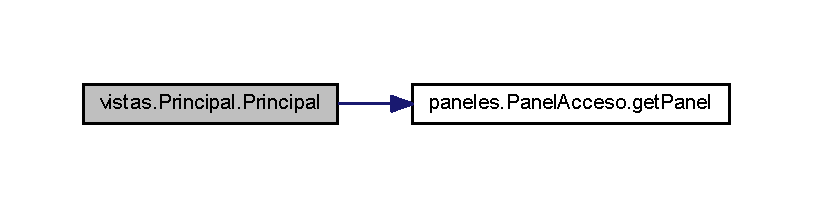
\includegraphics[width=350pt]{classvistas_1_1_principal_acf014fac1f15c33d980e722fe1e6d58f_cgraph}
\end{center}
\end{figure}


\subsection{Member Function Documentation}
\mbox{\Hypertarget{classvistas_1_1_principal_a0f01204c3cdf3b88718a5f2c6a6d9ac9}\label{classvistas_1_1_principal_a0f01204c3cdf3b88718a5f2c6a6d9ac9}} 
\index{vistas\+::\+Principal@{vistas\+::\+Principal}!cambiar\+Panel@{cambiar\+Panel}}
\index{cambiar\+Panel@{cambiar\+Panel}!vistas\+::\+Principal@{vistas\+::\+Principal}}
\subsubsection{\texorpdfstring{cambiar\+Panel()}{cambiarPanel()}}
{\footnotesize\ttfamily void vistas.\+Principal.\+cambiar\+Panel (\begin{DoxyParamCaption}\item[{J\+Panel}]{panel }\end{DoxyParamCaption})}



Definition at line 65 of file Principal.\+java.

\mbox{\Hypertarget{classvistas_1_1_principal_a0823d729a42c384bf4afd30b60a3e468}\label{classvistas_1_1_principal_a0823d729a42c384bf4afd30b60a3e468}} 
\index{vistas\+::\+Principal@{vistas\+::\+Principal}!cambiar\+Panel\+Acceso@{cambiar\+Panel\+Acceso}}
\index{cambiar\+Panel\+Acceso@{cambiar\+Panel\+Acceso}!vistas\+::\+Principal@{vistas\+::\+Principal}}
\subsubsection{\texorpdfstring{cambiar\+Panel\+Acceso()}{cambiarPanelAcceso()}}
{\footnotesize\ttfamily void vistas.\+Principal.\+cambiar\+Panel\+Acceso (\begin{DoxyParamCaption}{ }\end{DoxyParamCaption})}



Definition at line 88 of file Principal.\+java.

Here is the call graph for this function\+:
\nopagebreak
\begin{figure}[H]
\begin{center}
\leavevmode
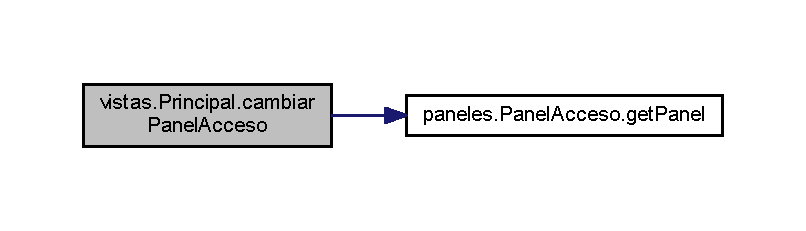
\includegraphics[width=350pt]{classvistas_1_1_principal_a0823d729a42c384bf4afd30b60a3e468_cgraph}
\end{center}
\end{figure}
\mbox{\Hypertarget{classvistas_1_1_principal_aa6783bab03cc60f1bf401d4c16293318}\label{classvistas_1_1_principal_aa6783bab03cc60f1bf401d4c16293318}} 
\index{vistas\+::\+Principal@{vistas\+::\+Principal}!cambiar\+Panel\+Compra@{cambiar\+Panel\+Compra}}
\index{cambiar\+Panel\+Compra@{cambiar\+Panel\+Compra}!vistas\+::\+Principal@{vistas\+::\+Principal}}
\subsubsection{\texorpdfstring{cambiar\+Panel\+Compra()}{cambiarPanelCompra()}}
{\footnotesize\ttfamily void vistas.\+Principal.\+cambiar\+Panel\+Compra (\begin{DoxyParamCaption}{ }\end{DoxyParamCaption})}



Definition at line 72 of file Principal.\+java.

Here is the call graph for this function\+:
\nopagebreak
\begin{figure}[H]
\begin{center}
\leavevmode
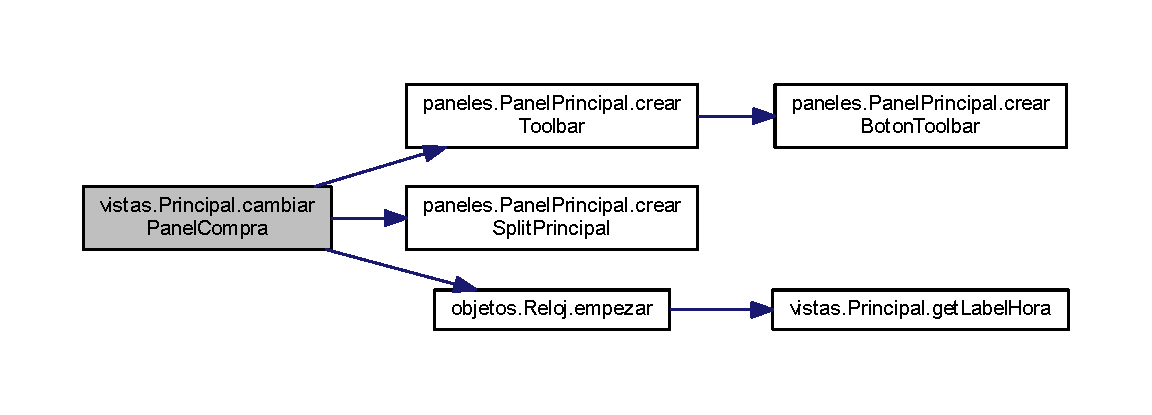
\includegraphics[width=350pt]{classvistas_1_1_principal_aa6783bab03cc60f1bf401d4c16293318_cgraph}
\end{center}
\end{figure}
\mbox{\Hypertarget{classvistas_1_1_principal_ad7379276c979124d4386d01439f24b42}\label{classvistas_1_1_principal_ad7379276c979124d4386d01439f24b42}} 
\index{vistas\+::\+Principal@{vistas\+::\+Principal}!get\+Conexion\+BD@{get\+Conexion\+BD}}
\index{get\+Conexion\+BD@{get\+Conexion\+BD}!vistas\+::\+Principal@{vistas\+::\+Principal}}
\subsubsection{\texorpdfstring{get\+Conexion\+B\+D()}{getConexionBD()}}
{\footnotesize\ttfamily \mbox{\hyperlink{classmysql_1_1_conexion_j_d_b_c}{Conexion\+J\+D\+BC}} vistas.\+Principal.\+get\+Conexion\+BD (\begin{DoxyParamCaption}{ }\end{DoxyParamCaption})}



Definition at line 118 of file Principal.\+java.

\mbox{\Hypertarget{classvistas_1_1_principal_a95e7bccba557226e9e56211a58a2e03c}\label{classvistas_1_1_principal_a95e7bccba557226e9e56211a58a2e03c}} 
\index{vistas\+::\+Principal@{vistas\+::\+Principal}!get\+Label\+Hora@{get\+Label\+Hora}}
\index{get\+Label\+Hora@{get\+Label\+Hora}!vistas\+::\+Principal@{vistas\+::\+Principal}}
\subsubsection{\texorpdfstring{get\+Label\+Hora()}{getLabelHora()}}
{\footnotesize\ttfamily J\+Label vistas.\+Principal.\+get\+Label\+Hora (\begin{DoxyParamCaption}{ }\end{DoxyParamCaption})}



Definition at line 106 of file Principal.\+java.

\mbox{\Hypertarget{classvistas_1_1_principal_a546a7dca6785535d3f48f5a7b43c20a1}\label{classvistas_1_1_principal_a546a7dca6785535d3f48f5a7b43c20a1}} 
\index{vistas\+::\+Principal@{vistas\+::\+Principal}!get\+Panel\+Principal@{get\+Panel\+Principal}}
\index{get\+Panel\+Principal@{get\+Panel\+Principal}!vistas\+::\+Principal@{vistas\+::\+Principal}}
\subsubsection{\texorpdfstring{get\+Panel\+Principal()}{getPanelPrincipal()}}
{\footnotesize\ttfamily \mbox{\hyperlink{classpaneles_1_1_panel_principal}{Panel\+Principal}} vistas.\+Principal.\+get\+Panel\+Principal (\begin{DoxyParamCaption}{ }\end{DoxyParamCaption})}



Definition at line 98 of file Principal.\+java.

\mbox{\Hypertarget{classvistas_1_1_principal_af7ea8d6ba599873466968add34233be0}\label{classvistas_1_1_principal_af7ea8d6ba599873466968add34233be0}} 
\index{vistas\+::\+Principal@{vistas\+::\+Principal}!get\+Usuario\+Actual@{get\+Usuario\+Actual}}
\index{get\+Usuario\+Actual@{get\+Usuario\+Actual}!vistas\+::\+Principal@{vistas\+::\+Principal}}
\subsubsection{\texorpdfstring{get\+Usuario\+Actual()}{getUsuarioActual()}}
{\footnotesize\ttfamily \mbox{\hyperlink{classobjetos_1_1_usuario}{Usuario}} vistas.\+Principal.\+get\+Usuario\+Actual (\begin{DoxyParamCaption}{ }\end{DoxyParamCaption})}



Definition at line 110 of file Principal.\+java.

\mbox{\Hypertarget{classvistas_1_1_principal_afc2c81827c88c9c2494b3345264e747d}\label{classvistas_1_1_principal_afc2c81827c88c9c2494b3345264e747d}} 
\index{vistas\+::\+Principal@{vistas\+::\+Principal}!get\+Ventana\+Principal@{get\+Ventana\+Principal}}
\index{get\+Ventana\+Principal@{get\+Ventana\+Principal}!vistas\+::\+Principal@{vistas\+::\+Principal}}
\subsubsection{\texorpdfstring{get\+Ventana\+Principal()}{getVentanaPrincipal()}}
{\footnotesize\ttfamily J\+Frame vistas.\+Principal.\+get\+Ventana\+Principal (\begin{DoxyParamCaption}{ }\end{DoxyParamCaption})}



Definition at line 102 of file Principal.\+java.

\mbox{\Hypertarget{classvistas_1_1_principal_a626dbf26bfdd3a03a2c1c99e34d25b6c}\label{classvistas_1_1_principal_a626dbf26bfdd3a03a2c1c99e34d25b6c}} 
\index{vistas\+::\+Principal@{vistas\+::\+Principal}!main@{main}}
\index{main@{main}!vistas\+::\+Principal@{vistas\+::\+Principal}}
\subsubsection{\texorpdfstring{main()}{main()}}
{\footnotesize\ttfamily static void vistas.\+Principal.\+main (\begin{DoxyParamCaption}\item[{String \mbox{[}$\,$\mbox{]}}]{args }\end{DoxyParamCaption})\hspace{0.3cm}{\ttfamily [static]}}



Definition at line 122 of file Principal.\+java.

Here is the call graph for this function\+:
\nopagebreak
\begin{figure}[H]
\begin{center}
\leavevmode
\includegraphics[width=350pt]{classvistas_1_1_principal_a626dbf26bfdd3a03a2c1c99e34d25b6c_cgraph}
\end{center}
\end{figure}
\mbox{\Hypertarget{classvistas_1_1_principal_a6f45e56ee7c99715b798ff202bd57d7e}\label{classvistas_1_1_principal_a6f45e56ee7c99715b798ff202bd57d7e}} 
\index{vistas\+::\+Principal@{vistas\+::\+Principal}!set\+Usuario\+Actual@{set\+Usuario\+Actual}}
\index{set\+Usuario\+Actual@{set\+Usuario\+Actual}!vistas\+::\+Principal@{vistas\+::\+Principal}}
\subsubsection{\texorpdfstring{set\+Usuario\+Actual()}{setUsuarioActual()}}
{\footnotesize\ttfamily void vistas.\+Principal.\+set\+Usuario\+Actual (\begin{DoxyParamCaption}\item[{\mbox{\hyperlink{classobjetos_1_1_usuario}{Usuario}}}]{usuario\+Actual }\end{DoxyParamCaption})}



Definition at line 114 of file Principal.\+java.



The documentation for this class was generated from the following file\+:\begin{DoxyCompactItemize}
\item 
C\+:/\+Users/jonmu/\+Desktop/\+P\+O\+P\+B\+L 4/src/vistas/\mbox{\hyperlink{_principal_8java}{Principal.\+java}}\end{DoxyCompactItemize}

\hypertarget{classobjetos_1_1_producto}{}\section{objetos.\+Producto Class Reference}
\label{classobjetos_1_1_producto}\index{objetos.\+Producto@{objetos.\+Producto}}
\subsection*{Public Member Functions}
\begin{DoxyCompactItemize}
\item 
\mbox{\Hypertarget{classobjetos_1_1_producto_a2944862f9387c43686583f85fdb9f79f}\label{classobjetos_1_1_producto_a2944862f9387c43686583f85fdb9f79f}} 
{\bfseries Producto} (double precio, String nombre, String descripcion, int id, int cantidad)
\item 
\mbox{\Hypertarget{classobjetos_1_1_producto_aca1868670a4e90738389af3bb5fa3e00}\label{classobjetos_1_1_producto_aca1868670a4e90738389af3bb5fa3e00}} 
void {\bfseries calcular\+Total} ()
\item 
\mbox{\Hypertarget{classobjetos_1_1_producto_afb28a08655f512fd3048a20281cbba44}\label{classobjetos_1_1_producto_afb28a08655f512fd3048a20281cbba44}} 
void {\bfseries incrementar\+Cantidad} ()
\item 
\mbox{\Hypertarget{classobjetos_1_1_producto_a6f54f8859ba9713ddb89fd082e811bd8}\label{classobjetos_1_1_producto_a6f54f8859ba9713ddb89fd082e811bd8}} 
Class$<$?$>$ {\bfseries get\+Field\+Class} (int indice)
\item 
\mbox{\Hypertarget{classobjetos_1_1_producto_a5857c7b25c0113cf682c7ea25a667fab}\label{classobjetos_1_1_producto_a5857c7b25c0113cf682c7ea25a667fab}} 
Object {\bfseries get\+Field\+At} (int columna)
\item 
\mbox{\Hypertarget{classobjetos_1_1_producto_a33cadb40029d686345420c930bcabacf}\label{classobjetos_1_1_producto_a33cadb40029d686345420c930bcabacf}} 
int {\bfseries get\+Cantidad} ()
\item 
\mbox{\Hypertarget{classobjetos_1_1_producto_ae14dcc26bdc312a512627177d4e7e442}\label{classobjetos_1_1_producto_ae14dcc26bdc312a512627177d4e7e442}} 
void {\bfseries set\+Cantidad} (int cantidad)
\item 
\mbox{\Hypertarget{classobjetos_1_1_producto_aa4b79134d6f59058f663c5e241bd6389}\label{classobjetos_1_1_producto_aa4b79134d6f59058f663c5e241bd6389}} 
double {\bfseries get\+Precio} ()
\item 
\mbox{\Hypertarget{classobjetos_1_1_producto_adbea45187ac465c2a7a2993f4739cb40}\label{classobjetos_1_1_producto_adbea45187ac465c2a7a2993f4739cb40}} 
double {\bfseries get\+Total} ()
\item 
\mbox{\Hypertarget{classobjetos_1_1_producto_a57f2351473e89e49d44441154f6110ed}\label{classobjetos_1_1_producto_a57f2351473e89e49d44441154f6110ed}} 
String {\bfseries get\+Nombre} ()
\item 
\mbox{\Hypertarget{classobjetos_1_1_producto_a47b9a05a0e7a504aaa56564c1b146927}\label{classobjetos_1_1_producto_a47b9a05a0e7a504aaa56564c1b146927}} 
String {\bfseries get\+Descripcion} ()
\item 
\mbox{\Hypertarget{classobjetos_1_1_producto_a60da2dbd5b5666a42c88295cf72fc193}\label{classobjetos_1_1_producto_a60da2dbd5b5666a42c88295cf72fc193}} 
int {\bfseries get\+ID} ()
\item 
\mbox{\Hypertarget{classobjetos_1_1_producto_a69f1b30e6711e637dbfd074c057adeee}\label{classobjetos_1_1_producto_a69f1b30e6711e637dbfd074c057adeee}} 
boolean {\bfseries equals} (Object obj)
\end{DoxyCompactItemize}


The documentation for this class was generated from the following file\+:\begin{DoxyCompactItemize}
\item 
C\+:/\+Users/jonmu/\+Desktop/\+P\+O\+P\+B\+L 4/src/objetos/Producto.\+java\end{DoxyCompactItemize}

\hypertarget{classobjetos_1_1_reloj}{}\section{objetos.\+Reloj Class Reference}
\label{classobjetos_1_1_reloj}\index{objetos.\+Reloj@{objetos.\+Reloj}}


Collaboration diagram for objetos.\+Reloj\+:
% FIG 0
\subsection*{Public Member Functions}
\begin{DoxyCompactItemize}
\item 
\mbox{\Hypertarget{classobjetos_1_1_reloj_aa15ad3d750972a2e0778c54b07847b1a}\label{classobjetos_1_1_reloj_aa15ad3d750972a2e0778c54b07847b1a}} 
{\bfseries Reloj} (\mbox{\hyperlink{classvistas_1_1_principal}{Principal}} principal)
\item 
\mbox{\Hypertarget{classobjetos_1_1_reloj_a8568b99d4457c01294d2078b033330a4}\label{classobjetos_1_1_reloj_a8568b99d4457c01294d2078b033330a4}} 
void {\bfseries empezar} ()
\end{DoxyCompactItemize}


The documentation for this class was generated from the following file\+:\begin{DoxyCompactItemize}
\item 
C\+:/\+Users/jonmu/\+Desktop/\+P\+O\+P\+B\+L 4/src/objetos/Reloj.\+java\end{DoxyCompactItemize}

\hypertarget{classlineaserie_1_1_serial_comm}{}\section{lineaserie.\+Serial\+Comm Class Reference}
\label{classlineaserie_1_1_serial_comm}\index{lineaserie.\+Serial\+Comm@{lineaserie.\+Serial\+Comm}}


Collaboration diagram for lineaserie.\+Serial\+Comm\+:
\nopagebreak
\begin{figure}[H]
\begin{center}
\leavevmode
\includegraphics[width=350pt]{classlineaserie_1_1_serial_comm__coll__graph}
\end{center}
\end{figure}
\subsection*{Public Member Functions}
\begin{DoxyCompactItemize}
\item 
\mbox{\hyperlink{classlineaserie_1_1_serial_comm_af7acba71f36fc78ac2555f52cb6e6c91}{Serial\+Comm}} (\mbox{\hyperlink{classvistas_1_1_principal}{Principal}} principal)
\item 
void \mbox{\hyperlink{classlineaserie_1_1_serial_comm_a877035aa389c7d3ceef75f1927afd4d5}{conectar}} (Comm\+Port\+Identifier port\+Identifier)  throws Exception     
\item 
void \mbox{\hyperlink{classlineaserie_1_1_serial_comm_a9e5dc899a435cb7bbd14c50af1e69a9e}{leer}} ()  throws I\+O\+Exception, Class\+Not\+Found\+Exception, S\+Q\+L\+Exception     
\item 
void \mbox{\hyperlink{classlineaserie_1_1_serial_comm_aafba8fce6137b4b5a5e7795f07fef02c}{escribir}} (String msg)
\item 
Comm\+Port\+Identifier \mbox{\hyperlink{classlineaserie_1_1_serial_comm_ac940f6b749e1137f5f1233b320e0e46f}{encontrar\+Puerto}} ()
\item 
String \mbox{\hyperlink{classlineaserie_1_1_serial_comm_ae0ae445e9464e90c1f4ebe3e943d0788}{get\+Port\+Type\+Name}} (int port\+Type)
\item 
void \mbox{\hyperlink{classlineaserie_1_1_serial_comm_a4bc07b152edbc3d04b42677ee93e3504}{cerrar}} ()
\end{DoxyCompactItemize}


\subsection{Detailed Description}


Definition at line 13 of file Serial\+Comm.\+java.



\subsection{Constructor \& Destructor Documentation}
\mbox{\Hypertarget{classlineaserie_1_1_serial_comm_af7acba71f36fc78ac2555f52cb6e6c91}\label{classlineaserie_1_1_serial_comm_af7acba71f36fc78ac2555f52cb6e6c91}} 
\index{lineaserie\+::\+Serial\+Comm@{lineaserie\+::\+Serial\+Comm}!Serial\+Comm@{Serial\+Comm}}
\index{Serial\+Comm@{Serial\+Comm}!lineaserie\+::\+Serial\+Comm@{lineaserie\+::\+Serial\+Comm}}
\subsubsection{\texorpdfstring{Serial\+Comm()}{SerialComm()}}
{\footnotesize\ttfamily lineaserie.\+Serial\+Comm.\+Serial\+Comm (\begin{DoxyParamCaption}\item[{\mbox{\hyperlink{classvistas_1_1_principal}{Principal}}}]{principal }\end{DoxyParamCaption})}



Definition at line 19 of file Serial\+Comm.\+java.



\subsection{Member Function Documentation}
\mbox{\Hypertarget{classlineaserie_1_1_serial_comm_a4bc07b152edbc3d04b42677ee93e3504}\label{classlineaserie_1_1_serial_comm_a4bc07b152edbc3d04b42677ee93e3504}} 
\index{lineaserie\+::\+Serial\+Comm@{lineaserie\+::\+Serial\+Comm}!cerrar@{cerrar}}
\index{cerrar@{cerrar}!lineaserie\+::\+Serial\+Comm@{lineaserie\+::\+Serial\+Comm}}
\subsubsection{\texorpdfstring{cerrar()}{cerrar()}}
{\footnotesize\ttfamily void lineaserie.\+Serial\+Comm.\+cerrar (\begin{DoxyParamCaption}{ }\end{DoxyParamCaption})}



Definition at line 124 of file Serial\+Comm.\+java.

\mbox{\Hypertarget{classlineaserie_1_1_serial_comm_a877035aa389c7d3ceef75f1927afd4d5}\label{classlineaserie_1_1_serial_comm_a877035aa389c7d3ceef75f1927afd4d5}} 
\index{lineaserie\+::\+Serial\+Comm@{lineaserie\+::\+Serial\+Comm}!conectar@{conectar}}
\index{conectar@{conectar}!lineaserie\+::\+Serial\+Comm@{lineaserie\+::\+Serial\+Comm}}
\subsubsection{\texorpdfstring{conectar()}{conectar()}}
{\footnotesize\ttfamily void lineaserie.\+Serial\+Comm.\+conectar (\begin{DoxyParamCaption}\item[{Comm\+Port\+Identifier}]{port\+Identifier }\end{DoxyParamCaption}) throws Exception}



Definition at line 22 of file Serial\+Comm.\+java.

\mbox{\Hypertarget{classlineaserie_1_1_serial_comm_ac940f6b749e1137f5f1233b320e0e46f}\label{classlineaserie_1_1_serial_comm_ac940f6b749e1137f5f1233b320e0e46f}} 
\index{lineaserie\+::\+Serial\+Comm@{lineaserie\+::\+Serial\+Comm}!encontrar\+Puerto@{encontrar\+Puerto}}
\index{encontrar\+Puerto@{encontrar\+Puerto}!lineaserie\+::\+Serial\+Comm@{lineaserie\+::\+Serial\+Comm}}
\subsubsection{\texorpdfstring{encontrar\+Puerto()}{encontrarPuerto()}}
{\footnotesize\ttfamily Comm\+Port\+Identifier lineaserie.\+Serial\+Comm.\+encontrar\+Puerto (\begin{DoxyParamCaption}{ }\end{DoxyParamCaption})}



Definition at line 92 of file Serial\+Comm.\+java.

Here is the call graph for this function\+:
\nopagebreak
\begin{figure}[H]
\begin{center}
\leavevmode
\includegraphics[width=350pt]{classlineaserie_1_1_serial_comm_ac940f6b749e1137f5f1233b320e0e46f_cgraph}
\end{center}
\end{figure}
\mbox{\Hypertarget{classlineaserie_1_1_serial_comm_aafba8fce6137b4b5a5e7795f07fef02c}\label{classlineaserie_1_1_serial_comm_aafba8fce6137b4b5a5e7795f07fef02c}} 
\index{lineaserie\+::\+Serial\+Comm@{lineaserie\+::\+Serial\+Comm}!escribir@{escribir}}
\index{escribir@{escribir}!lineaserie\+::\+Serial\+Comm@{lineaserie\+::\+Serial\+Comm}}
\subsubsection{\texorpdfstring{escribir()}{escribir()}}
{\footnotesize\ttfamily void lineaserie.\+Serial\+Comm.\+escribir (\begin{DoxyParamCaption}\item[{String}]{msg }\end{DoxyParamCaption})}



Definition at line 81 of file Serial\+Comm.\+java.

\mbox{\Hypertarget{classlineaserie_1_1_serial_comm_ae0ae445e9464e90c1f4ebe3e943d0788}\label{classlineaserie_1_1_serial_comm_ae0ae445e9464e90c1f4ebe3e943d0788}} 
\index{lineaserie\+::\+Serial\+Comm@{lineaserie\+::\+Serial\+Comm}!get\+Port\+Type\+Name@{get\+Port\+Type\+Name}}
\index{get\+Port\+Type\+Name@{get\+Port\+Type\+Name}!lineaserie\+::\+Serial\+Comm@{lineaserie\+::\+Serial\+Comm}}
\subsubsection{\texorpdfstring{get\+Port\+Type\+Name()}{getPortTypeName()}}
{\footnotesize\ttfamily String lineaserie.\+Serial\+Comm.\+get\+Port\+Type\+Name (\begin{DoxyParamCaption}\item[{int}]{port\+Type }\end{DoxyParamCaption})}



Definition at line 106 of file Serial\+Comm.\+java.

\mbox{\Hypertarget{classlineaserie_1_1_serial_comm_a9e5dc899a435cb7bbd14c50af1e69a9e}\label{classlineaserie_1_1_serial_comm_a9e5dc899a435cb7bbd14c50af1e69a9e}} 
\index{lineaserie\+::\+Serial\+Comm@{lineaserie\+::\+Serial\+Comm}!leer@{leer}}
\index{leer@{leer}!lineaserie\+::\+Serial\+Comm@{lineaserie\+::\+Serial\+Comm}}
\subsubsection{\texorpdfstring{leer()}{leer()}}
{\footnotesize\ttfamily void lineaserie.\+Serial\+Comm.\+leer (\begin{DoxyParamCaption}{ }\end{DoxyParamCaption}) throws I\+O\+Exception, Class\+Not\+Found\+Exception, S\+Q\+L\+Exception}


\begin{DoxyExceptions}{Exceptions}
{\em I\+O\+Exception} & ~\newline
\\
\hline
{\em S\+Q\+L\+Exception} & \\
\hline
{\em Class\+Not\+Found\+Exception} & \\
\hline
\end{DoxyExceptions}


Definition at line 46 of file Serial\+Comm.\+java.

Here is the call graph for this function\+:
\nopagebreak
\begin{figure}[H]
\begin{center}
\leavevmode
\includegraphics[width=350pt]{classlineaserie_1_1_serial_comm_a9e5dc899a435cb7bbd14c50af1e69a9e_cgraph}
\end{center}
\end{figure}


The documentation for this class was generated from the following file\+:\begin{DoxyCompactItemize}
\item 
C\+:/\+Users/jonmu/\+Desktop/\+P\+O\+P\+B\+L 4/src/lineaserie/\mbox{\hyperlink{_serial_comm_8java}{Serial\+Comm.\+java}}\end{DoxyCompactItemize}

\hypertarget{classmodelos_1_1_trazador_tabla_maquina}{}\section{modelos.\+Trazador\+Tabla\+Maquina Class Reference}
\label{classmodelos_1_1_trazador_tabla_maquina}\index{modelos.\+Trazador\+Tabla\+Maquina@{modelos.\+Trazador\+Tabla\+Maquina}}


Inheritance diagram for modelos.\+Trazador\+Tabla\+Maquina\+:
% FIG 0


Collaboration diagram for modelos.\+Trazador\+Tabla\+Maquina\+:
% FIG 1
\subsection*{Public Member Functions}
\begin{DoxyCompactItemize}
\item 
\mbox{\Hypertarget{classmodelos_1_1_trazador_tabla_maquina_a2ea391f01832f424c6e212bd8ff86484}\label{classmodelos_1_1_trazador_tabla_maquina_a2ea391f01832f424c6e212bd8ff86484}} 
Component {\bfseries get\+Table\+Cell\+Renderer\+Component} (J\+Table table, Object value, boolean is\+Selected, boolean has\+Focus, int row, int col)
\end{DoxyCompactItemize}


The documentation for this class was generated from the following file\+:\begin{DoxyCompactItemize}
\item 
C\+:/\+Users/jonmu/\+Desktop/\+P\+O\+P\+B\+L 4/src/modelos/Trazador\+Tabla\+Maquina.\+java\end{DoxyCompactItemize}

\hypertarget{classrenderer_1_1_trazador_tabla_productos}{}\section{renderer.\+Trazador\+Tabla\+Productos Class Reference}
\label{classrenderer_1_1_trazador_tabla_productos}\index{renderer.\+Trazador\+Tabla\+Productos@{renderer.\+Trazador\+Tabla\+Productos}}


Inheritance diagram for renderer.\+Trazador\+Tabla\+Productos\+:
% FIG 0


Collaboration diagram for renderer.\+Trazador\+Tabla\+Productos\+:
% FIG 1
\subsection*{Public Member Functions}
\begin{DoxyCompactItemize}
\item 
\mbox{\Hypertarget{classrenderer_1_1_trazador_tabla_productos_a0d15ae9262431f81b66258d7f445092c}\label{classrenderer_1_1_trazador_tabla_productos_a0d15ae9262431f81b66258d7f445092c}} 
Component {\bfseries get\+Table\+Cell\+Renderer\+Component} (J\+Table table, Object valor, boolean is\+Selected, boolean has\+Focus, int fila, int columna)
\end{DoxyCompactItemize}


The documentation for this class was generated from the following file\+:\begin{DoxyCompactItemize}
\item 
C\+:/\+Users/jonmu/\+Desktop/\+P\+O\+P\+B\+L 4/src/renderer/Trazador\+Tabla\+Productos.\+java\end{DoxyCompactItemize}

\hypertarget{classobjetos_1_1_usuario}{}\section{objetos.\+Usuario Class Reference}
\label{classobjetos_1_1_usuario}\index{objetos.\+Usuario@{objetos.\+Usuario}}


Collaboration diagram for objetos.\+Usuario\+:
% FIG 0
\subsection*{Public Member Functions}
\begin{DoxyCompactItemize}
\item 
\mbox{\Hypertarget{classobjetos_1_1_usuario_a0d13573d3c808402df18a489ecb81654}\label{classobjetos_1_1_usuario_a0d13573d3c808402df18a489ecb81654}} 
{\bfseries Usuario} (String usuario, String password, String nombre, String apellido1, String apellido2, String email, String fecha\+\_\+nacimiento, String poblacion, String codigo\+\_\+postal, String direccion, String iban, String genero, String telefono, String dni)
\item 
\mbox{\Hypertarget{classobjetos_1_1_usuario_aa3a7114995ef02ed515c668148eb2aca}\label{classobjetos_1_1_usuario_aa3a7114995ef02ed515c668148eb2aca}} 
{\bfseries Usuario} (String usuario, boolean es\+Admin)
\item 
\mbox{\Hypertarget{classobjetos_1_1_usuario_a1d3a6e897c852226d1b419c67089ec3b}\label{classobjetos_1_1_usuario_a1d3a6e897c852226d1b419c67089ec3b}} 
void {\bfseries agregar\+Pedido} (\mbox{\hyperlink{classobjetos_1_1_pedido}{Pedido}} p)
\item 
\mbox{\Hypertarget{classobjetos_1_1_usuario_af3fd03fa3c7765c9005a75d70256288e}\label{classobjetos_1_1_usuario_af3fd03fa3c7765c9005a75d70256288e}} 
List$<$ \mbox{\hyperlink{classobjetos_1_1_pedido}{Pedido}} $>$ {\bfseries get\+Lista\+Pedidos} ()
\item 
\mbox{\Hypertarget{classobjetos_1_1_usuario_ab7bc0d18ecfee488dcf322094629ef5d}\label{classobjetos_1_1_usuario_ab7bc0d18ecfee488dcf322094629ef5d}} 
void {\bfseries set\+Lista\+Pedidos} (List$<$ \mbox{\hyperlink{classobjetos_1_1_pedido}{Pedido}} $>$ lista\+Pedidos)
\item 
\mbox{\Hypertarget{classobjetos_1_1_usuario_a7be3dc8fe52e00029ec3a6ec763116e1}\label{classobjetos_1_1_usuario_a7be3dc8fe52e00029ec3a6ec763116e1}} 
void {\bfseries set\+Usuario} (String usuario)
\item 
\mbox{\Hypertarget{classobjetos_1_1_usuario_acebc98a73bf17db1fb88e476e64f2c6c}\label{classobjetos_1_1_usuario_acebc98a73bf17db1fb88e476e64f2c6c}} 
void {\bfseries set\+Password} (String password)
\item 
\mbox{\Hypertarget{classobjetos_1_1_usuario_af80f3d60addfde641e49e66e6a1f5f8e}\label{classobjetos_1_1_usuario_af80f3d60addfde641e49e66e6a1f5f8e}} 
void {\bfseries set\+Nombre} (String nombre)
\item 
\mbox{\Hypertarget{classobjetos_1_1_usuario_a705188b9b04c0e4cfcad7f2973f7673e}\label{classobjetos_1_1_usuario_a705188b9b04c0e4cfcad7f2973f7673e}} 
void {\bfseries set\+Apellido1} (String apellido1)
\item 
\mbox{\Hypertarget{classobjetos_1_1_usuario_a73a071e063ba33c64d1453bf788b1d2f}\label{classobjetos_1_1_usuario_a73a071e063ba33c64d1453bf788b1d2f}} 
void {\bfseries set\+Apellido2} (String apellido2)
\item 
\mbox{\Hypertarget{classobjetos_1_1_usuario_ad64ef1b4bc35e4039e9e5f31d651e043}\label{classobjetos_1_1_usuario_ad64ef1b4bc35e4039e9e5f31d651e043}} 
void {\bfseries set\+Email} (String email)
\item 
\mbox{\Hypertarget{classobjetos_1_1_usuario_a5d99fa41f8ec817e0eca78ef718a3771}\label{classobjetos_1_1_usuario_a5d99fa41f8ec817e0eca78ef718a3771}} 
void {\bfseries set\+Fecha\+\_\+nacimiento} (String fecha\+\_\+nacimiento)
\item 
\mbox{\Hypertarget{classobjetos_1_1_usuario_a617d6485d3c99725d35a7f37093a72cf}\label{classobjetos_1_1_usuario_a617d6485d3c99725d35a7f37093a72cf}} 
void {\bfseries set\+Direccion} (String direccion)
\item 
\mbox{\Hypertarget{classobjetos_1_1_usuario_a1dd10cd5dfebcd7cf424a877839c1079}\label{classobjetos_1_1_usuario_a1dd10cd5dfebcd7cf424a877839c1079}} 
void {\bfseries set\+Iban} (String iban)
\item 
\mbox{\Hypertarget{classobjetos_1_1_usuario_ac9905e666ce288e519fc087e23d25854}\label{classobjetos_1_1_usuario_ac9905e666ce288e519fc087e23d25854}} 
void {\bfseries set\+Genero} (String genero)
\item 
\mbox{\Hypertarget{classobjetos_1_1_usuario_a0ff938bea2a54afe1c1692e8944010e7}\label{classobjetos_1_1_usuario_a0ff938bea2a54afe1c1692e8944010e7}} 
void {\bfseries set\+Telefono} (String telefono)
\item 
\mbox{\Hypertarget{classobjetos_1_1_usuario_a091d44abe53530995ec78cde4c574a1d}\label{classobjetos_1_1_usuario_a091d44abe53530995ec78cde4c574a1d}} 
String {\bfseries get\+Usuario} ()
\item 
\mbox{\Hypertarget{classobjetos_1_1_usuario_a78a59647b3bfd56744741973ff9521ff}\label{classobjetos_1_1_usuario_a78a59647b3bfd56744741973ff9521ff}} 
String {\bfseries get\+Password} ()
\item 
\mbox{\Hypertarget{classobjetos_1_1_usuario_a055ad022318e4a768f4586d7a114653d}\label{classobjetos_1_1_usuario_a055ad022318e4a768f4586d7a114653d}} 
String {\bfseries get\+Nombre} ()
\item 
\mbox{\Hypertarget{classobjetos_1_1_usuario_ae9882e1900abade7ade510479c9f8383}\label{classobjetos_1_1_usuario_ae9882e1900abade7ade510479c9f8383}} 
String {\bfseries get\+Apellido1} ()
\item 
\mbox{\Hypertarget{classobjetos_1_1_usuario_a1d3064bdecaadd7ff0487f0715780ee5}\label{classobjetos_1_1_usuario_a1d3064bdecaadd7ff0487f0715780ee5}} 
String {\bfseries get\+Apellido2} ()
\item 
\mbox{\Hypertarget{classobjetos_1_1_usuario_a504d7bcb1c63297b870f8499b88381d1}\label{classobjetos_1_1_usuario_a504d7bcb1c63297b870f8499b88381d1}} 
String {\bfseries get\+Email} ()
\item 
\mbox{\Hypertarget{classobjetos_1_1_usuario_a175efa1135100c4750a19be789391307}\label{classobjetos_1_1_usuario_a175efa1135100c4750a19be789391307}} 
String {\bfseries get\+Fecha\+\_\+nacimiento} ()
\item 
\mbox{\Hypertarget{classobjetos_1_1_usuario_a3e13dfa01d027561e7866f4cd1c2e3c5}\label{classobjetos_1_1_usuario_a3e13dfa01d027561e7866f4cd1c2e3c5}} 
String {\bfseries get\+Direccion} ()
\item 
\mbox{\Hypertarget{classobjetos_1_1_usuario_ab66729eaad2e417c447f8b86bb56c986}\label{classobjetos_1_1_usuario_ab66729eaad2e417c447f8b86bb56c986}} 
String {\bfseries get\+Iban} ()
\item 
\mbox{\Hypertarget{classobjetos_1_1_usuario_ad91ec5ebca29f02270f825af722dd285}\label{classobjetos_1_1_usuario_ad91ec5ebca29f02270f825af722dd285}} 
String {\bfseries get\+Genero} ()
\item 
\mbox{\Hypertarget{classobjetos_1_1_usuario_a61da31ecd6448c2064a7dcd276d71754}\label{classobjetos_1_1_usuario_a61da31ecd6448c2064a7dcd276d71754}} 
String {\bfseries get\+Telefono} ()
\item 
\mbox{\Hypertarget{classobjetos_1_1_usuario_a110d1f830d1c6041f1ee78c5bd32395d}\label{classobjetos_1_1_usuario_a110d1f830d1c6041f1ee78c5bd32395d}} 
boolean {\bfseries get\+Es\+Admin} ()
\item 
\mbox{\Hypertarget{classobjetos_1_1_usuario_ac5bbdb911746e90bb9d0be80195eb425}\label{classobjetos_1_1_usuario_ac5bbdb911746e90bb9d0be80195eb425}} 
String {\bfseries get\+Poblacion} ()
\item 
\mbox{\Hypertarget{classobjetos_1_1_usuario_a7e8a422150526d3436159d63817c225d}\label{classobjetos_1_1_usuario_a7e8a422150526d3436159d63817c225d}} 
String {\bfseries get\+Codigo\+\_\+postal} ()
\item 
\mbox{\Hypertarget{classobjetos_1_1_usuario_a35aa11d09cd9caa12bb4e2445fe36c1f}\label{classobjetos_1_1_usuario_a35aa11d09cd9caa12bb4e2445fe36c1f}} 
String {\bfseries get\+Dni} ()
\item 
\mbox{\Hypertarget{classobjetos_1_1_usuario_a60bfdc7b6f95b380ed50723c1e9b1cc6}\label{classobjetos_1_1_usuario_a60bfdc7b6f95b380ed50723c1e9b1cc6}} 
String {\bfseries to\+String} ()
\end{DoxyCompactItemize}


The documentation for this class was generated from the following file\+:\begin{DoxyCompactItemize}
\item 
C\+:/\+Users/jonmu/\+Desktop/\+P\+O\+P\+B\+L 4/src/objetos/Usuario.\+java\end{DoxyCompactItemize}

\chapter{File Documentation}
\hypertarget{_controlador_acceso_8java}{}\section{C\+:/\+Users/jonmu/\+Desktop/\+P\+O\+P\+BL 4/src/controladores/\+Controlador\+Acceso.java File Reference}
\label{_controlador_acceso_8java}\index{C\+:/\+Users/jonmu/\+Desktop/\+P\+O\+P\+B\+L 4/src/controladores/\+Controlador\+Acceso.\+java@{C\+:/\+Users/jonmu/\+Desktop/\+P\+O\+P\+B\+L 4/src/controladores/\+Controlador\+Acceso.\+java}}
\subsection*{Classes}
\begin{DoxyCompactItemize}
\item 
class \mbox{\hyperlink{classcontroladores_1_1_controlador_acceso}{controladores.\+Controlador\+Acceso}}
\end{DoxyCompactItemize}
\subsection*{Packages}
\begin{DoxyCompactItemize}
\item 
package \mbox{\hyperlink{namespacecontroladores}{controladores}}
\end{DoxyCompactItemize}

\hypertarget{_controlador_menu_admin_8java}{}\section{C\+:/\+Users/jonmu/\+Desktop/\+P\+O\+P\+BL 4/src/controladores/\+Controlador\+Menu\+Admin.java File Reference}
\label{_controlador_menu_admin_8java}\index{C\+:/\+Users/jonmu/\+Desktop/\+P\+O\+P\+B\+L 4/src/controladores/\+Controlador\+Menu\+Admin.\+java@{C\+:/\+Users/jonmu/\+Desktop/\+P\+O\+P\+B\+L 4/src/controladores/\+Controlador\+Menu\+Admin.\+java}}
\subsection*{Classes}
\begin{DoxyCompactItemize}
\item 
class \mbox{\hyperlink{classcontroladores_1_1_controlador_menu_admin}{controladores.\+Controlador\+Menu\+Admin}}
\end{DoxyCompactItemize}
\subsection*{Packages}
\begin{DoxyCompactItemize}
\item 
package \mbox{\hyperlink{namespacecontroladores}{controladores}}
\end{DoxyCompactItemize}

\hypertarget{_controlador_tabla_principal_8java}{}\section{C\+:/\+Users/jonmu/\+Desktop/\+P\+O\+P\+BL 4/src/controladores/\+Controlador\+Tabla\+Principal.java File Reference}
\label{_controlador_tabla_principal_8java}\index{C\+:/\+Users/jonmu/\+Desktop/\+P\+O\+P\+B\+L 4/src/controladores/\+Controlador\+Tabla\+Principal.\+java@{C\+:/\+Users/jonmu/\+Desktop/\+P\+O\+P\+B\+L 4/src/controladores/\+Controlador\+Tabla\+Principal.\+java}}
\subsection*{Classes}
\begin{DoxyCompactItemize}
\item 
class \mbox{\hyperlink{classcontroladores_1_1_controlador_tabla_principal}{controladores.\+Controlador\+Tabla\+Principal}}
\end{DoxyCompactItemize}
\subsection*{Packages}
\begin{DoxyCompactItemize}
\item 
package \mbox{\hyperlink{namespacecontroladores}{controladores}}
\end{DoxyCompactItemize}

\hypertarget{_controlador_toolbar_8java}{}\section{C\+:/\+Users/jonmu/\+Desktop/\+P\+O\+P\+BL 4/src/controladores/\+Controlador\+Toolbar.java File Reference}
\label{_controlador_toolbar_8java}\index{C\+:/\+Users/jonmu/\+Desktop/\+P\+O\+P\+B\+L 4/src/controladores/\+Controlador\+Toolbar.\+java@{C\+:/\+Users/jonmu/\+Desktop/\+P\+O\+P\+B\+L 4/src/controladores/\+Controlador\+Toolbar.\+java}}
\subsection*{Classes}
\begin{DoxyCompactItemize}
\item 
class \mbox{\hyperlink{classcontroladores_1_1_controlador_toolbar}{controladores.\+Controlador\+Toolbar}}
\end{DoxyCompactItemize}
\subsection*{Packages}
\begin{DoxyCompactItemize}
\item 
package \mbox{\hyperlink{namespacecontroladores}{controladores}}
\end{DoxyCompactItemize}

\hypertarget{_imagenes_8java}{}\section{C\+:/\+Users/jonmu/\+Desktop/\+P\+O\+P\+BL 4/src/imagenes/\+Imagenes.java File Reference}
\label{_imagenes_8java}\index{C\+:/\+Users/jonmu/\+Desktop/\+P\+O\+P\+B\+L 4/src/imagenes/\+Imagenes.\+java@{C\+:/\+Users/jonmu/\+Desktop/\+P\+O\+P\+B\+L 4/src/imagenes/\+Imagenes.\+java}}
\subsection*{Classes}
\begin{DoxyCompactItemize}
\item 
class \mbox{\hyperlink{classimagenes_1_1_imagenes}{imagenes.\+Imagenes}}
\end{DoxyCompactItemize}
\subsection*{Packages}
\begin{DoxyCompactItemize}
\item 
package \mbox{\hyperlink{namespaceimagenes}{imagenes}}
\end{DoxyCompactItemize}

\hypertarget{_escritor_8java}{}\section{C\+:/\+Users/jonmu/\+Desktop/\+P\+O\+P\+BL 4/src/lineaserie/\+Escritor.java File Reference}
\label{_escritor_8java}\index{C\+:/\+Users/jonmu/\+Desktop/\+P\+O\+P\+B\+L 4/src/lineaserie/\+Escritor.\+java@{C\+:/\+Users/jonmu/\+Desktop/\+P\+O\+P\+B\+L 4/src/lineaserie/\+Escritor.\+java}}
\subsection*{Classes}
\begin{DoxyCompactItemize}
\item 
class \mbox{\hyperlink{classlineaserie_1_1_escritor}{lineaserie.\+Escritor}}
\end{DoxyCompactItemize}
\subsection*{Packages}
\begin{DoxyCompactItemize}
\item 
package \mbox{\hyperlink{namespacelineaserie}{lineaserie}}
\end{DoxyCompactItemize}

\hypertarget{_inicializador_8java}{}\section{C\+:/\+Users/jonmu/\+Desktop/\+P\+O\+P\+BL 4/src/lineaserie/\+Inicializador.java File Reference}
\label{_inicializador_8java}\index{C\+:/\+Users/jonmu/\+Desktop/\+P\+O\+P\+B\+L 4/src/lineaserie/\+Inicializador.\+java@{C\+:/\+Users/jonmu/\+Desktop/\+P\+O\+P\+B\+L 4/src/lineaserie/\+Inicializador.\+java}}
\subsection*{Classes}
\begin{DoxyCompactItemize}
\item 
class \mbox{\hyperlink{classlineaserie_1_1_inicializador}{lineaserie.\+Inicializador}}
\end{DoxyCompactItemize}
\subsection*{Packages}
\begin{DoxyCompactItemize}
\item 
package \mbox{\hyperlink{namespacelineaserie}{lineaserie}}
\end{DoxyCompactItemize}

\hypertarget{_lector_8java}{}\section{C\+:/\+Users/jonmu/\+Desktop/\+P\+O\+P\+BL 4/src/lineaserie/\+Lector.java File Reference}
\label{_lector_8java}\index{C\+:/\+Users/jonmu/\+Desktop/\+P\+O\+P\+B\+L 4/src/lineaserie/\+Lector.\+java@{C\+:/\+Users/jonmu/\+Desktop/\+P\+O\+P\+B\+L 4/src/lineaserie/\+Lector.\+java}}
\subsection*{Classes}
\begin{DoxyCompactItemize}
\item 
class \mbox{\hyperlink{classlineaserie_1_1_lector}{lineaserie.\+Lector}}
\end{DoxyCompactItemize}
\subsection*{Packages}
\begin{DoxyCompactItemize}
\item 
package \mbox{\hyperlink{namespacelineaserie}{lineaserie}}
\end{DoxyCompactItemize}

\hypertarget{_serial_comm_8java}{}\section{C\+:/\+Users/jonmu/\+Desktop/\+P\+O\+P\+BL 4/src/lineaserie/\+Serial\+Comm.java File Reference}
\label{_serial_comm_8java}\index{C\+:/\+Users/jonmu/\+Desktop/\+P\+O\+P\+B\+L 4/src/lineaserie/\+Serial\+Comm.\+java@{C\+:/\+Users/jonmu/\+Desktop/\+P\+O\+P\+B\+L 4/src/lineaserie/\+Serial\+Comm.\+java}}
\subsection*{Classes}
\begin{DoxyCompactItemize}
\item 
class \mbox{\hyperlink{classlineaserie_1_1_serial_comm}{lineaserie.\+Serial\+Comm}}
\end{DoxyCompactItemize}
\subsection*{Packages}
\begin{DoxyCompactItemize}
\item 
package \mbox{\hyperlink{namespacelineaserie}{lineaserie}}
\end{DoxyCompactItemize}

\hypertarget{_modelo_columnas_tabla_8java}{}\section{C\+:/\+Users/jonmu/\+Desktop/\+P\+O\+P\+BL 4/src/modelos/\+Modelo\+Columnas\+Tabla.java File Reference}
\label{_modelo_columnas_tabla_8java}\index{C\+:/\+Users/jonmu/\+Desktop/\+P\+O\+P\+B\+L 4/src/modelos/\+Modelo\+Columnas\+Tabla.\+java@{C\+:/\+Users/jonmu/\+Desktop/\+P\+O\+P\+B\+L 4/src/modelos/\+Modelo\+Columnas\+Tabla.\+java}}
\subsection*{Classes}
\begin{DoxyCompactItemize}
\item 
class \mbox{\hyperlink{classmodelos_1_1_modelo_columnas_tabla}{modelos.\+Modelo\+Columnas\+Tabla}}
\end{DoxyCompactItemize}
\subsection*{Packages}
\begin{DoxyCompactItemize}
\item 
package \mbox{\hyperlink{namespacemodelos}{modelos}}
\end{DoxyCompactItemize}

\hypertarget{_modelo_columnas_tabla_productos_8java}{}\section{C\+:/\+Users/jonmu/\+Desktop/\+P\+O\+P\+BL 4/src/modelos/\+Modelo\+Columnas\+Tabla\+Productos.java File Reference}
\label{_modelo_columnas_tabla_productos_8java}\index{C\+:/\+Users/jonmu/\+Desktop/\+P\+O\+P\+B\+L 4/src/modelos/\+Modelo\+Columnas\+Tabla\+Productos.\+java@{C\+:/\+Users/jonmu/\+Desktop/\+P\+O\+P\+B\+L 4/src/modelos/\+Modelo\+Columnas\+Tabla\+Productos.\+java}}
\subsection*{Classes}
\begin{DoxyCompactItemize}
\item 
class \mbox{\hyperlink{classmodelos_1_1_modelo_columnas_tabla_productos}{modelos.\+Modelo\+Columnas\+Tabla\+Productos}}
\end{DoxyCompactItemize}
\subsection*{Packages}
\begin{DoxyCompactItemize}
\item 
package \mbox{\hyperlink{namespacemodelos}{modelos}}
\end{DoxyCompactItemize}

\hypertarget{_modelo_pedidos_8java}{}\section{C\+:/\+Users/jonmu/\+Desktop/\+P\+O\+P\+BL 4/src/modelos/\+Modelo\+Pedidos.java File Reference}
\label{_modelo_pedidos_8java}\index{C\+:/\+Users/jonmu/\+Desktop/\+P\+O\+P\+B\+L 4/src/modelos/\+Modelo\+Pedidos.\+java@{C\+:/\+Users/jonmu/\+Desktop/\+P\+O\+P\+B\+L 4/src/modelos/\+Modelo\+Pedidos.\+java}}
\subsection*{Classes}
\begin{DoxyCompactItemize}
\item 
class \mbox{\hyperlink{classmodelos_1_1_modelo_pedidos}{modelos.\+Modelo\+Pedidos}}
\end{DoxyCompactItemize}
\subsection*{Packages}
\begin{DoxyCompactItemize}
\item 
package \mbox{\hyperlink{namespacemodelos}{modelos}}
\end{DoxyCompactItemize}

\hypertarget{_modelo_tabla_maquina_8java}{}\section{C\+:/\+Users/jonmu/\+Desktop/\+P\+O\+P\+BL 4/src/modelos/\+Modelo\+Tabla\+Maquina.java File Reference}
\label{_modelo_tabla_maquina_8java}\index{C\+:/\+Users/jonmu/\+Desktop/\+P\+O\+P\+B\+L 4/src/modelos/\+Modelo\+Tabla\+Maquina.\+java@{C\+:/\+Users/jonmu/\+Desktop/\+P\+O\+P\+B\+L 4/src/modelos/\+Modelo\+Tabla\+Maquina.\+java}}
\subsection*{Classes}
\begin{DoxyCompactItemize}
\item 
class \mbox{\hyperlink{classmodelos_1_1_modelo_tabla_maquina}{modelos.\+Modelo\+Tabla\+Maquina}}
\end{DoxyCompactItemize}
\subsection*{Packages}
\begin{DoxyCompactItemize}
\item 
package \mbox{\hyperlink{namespacemodelos}{modelos}}
\end{DoxyCompactItemize}

\hypertarget{_modelo_tabla_productos_8java}{}\section{C\+:/\+Users/jonmu/\+Desktop/\+P\+O\+P\+BL 4/src/modelos/\+Modelo\+Tabla\+Productos.java File Reference}
\label{_modelo_tabla_productos_8java}\index{C\+:/\+Users/jonmu/\+Desktop/\+P\+O\+P\+B\+L 4/src/modelos/\+Modelo\+Tabla\+Productos.\+java@{C\+:/\+Users/jonmu/\+Desktop/\+P\+O\+P\+B\+L 4/src/modelos/\+Modelo\+Tabla\+Productos.\+java}}
\subsection*{Classes}
\begin{DoxyCompactItemize}
\item 
class \mbox{\hyperlink{classmodelos_1_1_modelo_tabla_productos}{modelos.\+Modelo\+Tabla\+Productos}}
\end{DoxyCompactItemize}
\subsection*{Packages}
\begin{DoxyCompactItemize}
\item 
package \mbox{\hyperlink{namespacemodelos}{modelos}}
\end{DoxyCompactItemize}

\hypertarget{_modelo_usuarios_8java}{}\section{C\+:/\+Users/jonmu/\+Desktop/\+P\+O\+P\+BL 4/src/modelos/\+Modelo\+Usuarios.java File Reference}
\label{_modelo_usuarios_8java}\index{C\+:/\+Users/jonmu/\+Desktop/\+P\+O\+P\+B\+L 4/src/modelos/\+Modelo\+Usuarios.\+java@{C\+:/\+Users/jonmu/\+Desktop/\+P\+O\+P\+B\+L 4/src/modelos/\+Modelo\+Usuarios.\+java}}
\subsection*{Classes}
\begin{DoxyCompactItemize}
\item 
class \mbox{\hyperlink{classmodelos_1_1_modelo_usuarios}{modelos.\+Modelo\+Usuarios}}
\end{DoxyCompactItemize}
\subsection*{Packages}
\begin{DoxyCompactItemize}
\item 
package \mbox{\hyperlink{namespacemodelos}{modelos}}
\end{DoxyCompactItemize}

\hypertarget{_trazador_tabla_maquina_8java}{}\section{C\+:/\+Users/jonmu/\+Desktop/\+P\+O\+P\+BL 4/src/modelos/\+Trazador\+Tabla\+Maquina.java File Reference}
\label{_trazador_tabla_maquina_8java}\index{C\+:/\+Users/jonmu/\+Desktop/\+P\+O\+P\+B\+L 4/src/modelos/\+Trazador\+Tabla\+Maquina.\+java@{C\+:/\+Users/jonmu/\+Desktop/\+P\+O\+P\+B\+L 4/src/modelos/\+Trazador\+Tabla\+Maquina.\+java}}
\subsection*{Classes}
\begin{DoxyCompactItemize}
\item 
class \mbox{\hyperlink{classmodelos_1_1_trazador_tabla_maquina}{modelos.\+Trazador\+Tabla\+Maquina}}
\end{DoxyCompactItemize}
\subsection*{Packages}
\begin{DoxyCompactItemize}
\item 
package \mbox{\hyperlink{namespacemodelos}{modelos}}
\end{DoxyCompactItemize}

\hypertarget{_conexion_j_d_b_c_8java}{}\section{C\+:/\+Users/jonmu/\+Desktop/\+P\+O\+P\+BL 4/src/mysql/\+Conexion\+J\+D\+BC.java File Reference}
\label{_conexion_j_d_b_c_8java}\index{C\+:/\+Users/jonmu/\+Desktop/\+P\+O\+P\+B\+L 4/src/mysql/\+Conexion\+J\+D\+B\+C.\+java@{C\+:/\+Users/jonmu/\+Desktop/\+P\+O\+P\+B\+L 4/src/mysql/\+Conexion\+J\+D\+B\+C.\+java}}
\subsection*{Classes}
\begin{DoxyCompactItemize}
\item 
class \mbox{\hyperlink{classmysql_1_1_conexion_j_d_b_c}{mysql.\+Conexion\+J\+D\+BC}}
\end{DoxyCompactItemize}
\subsection*{Packages}
\begin{DoxyCompactItemize}
\item 
package \mbox{\hyperlink{namespacemysql}{mysql}}
\end{DoxyCompactItemize}

\hypertarget{_barcode_reader_8java}{}\section{C\+:/\+Users/jonmu/\+Desktop/\+P\+O\+P\+BL 4/src/objetos/\+Barcode\+Reader.java File Reference}
\label{_barcode_reader_8java}\index{C\+:/\+Users/jonmu/\+Desktop/\+P\+O\+P\+B\+L 4/src/objetos/\+Barcode\+Reader.\+java@{C\+:/\+Users/jonmu/\+Desktop/\+P\+O\+P\+B\+L 4/src/objetos/\+Barcode\+Reader.\+java}}
\subsection*{Classes}
\begin{DoxyCompactItemize}
\item 
class \mbox{\hyperlink{classobjetos_1_1_barcode_reader}{objetos.\+Barcode\+Reader}}
\item 
interface \mbox{\hyperlink{interfaceobjetos_1_1_barcode_reader_1_1_barcode_listener}{objetos.\+Barcode\+Reader.\+Barcode\+Listener}}
\end{DoxyCompactItemize}
\subsection*{Packages}
\begin{DoxyCompactItemize}
\item 
package \mbox{\hyperlink{namespaceobjetos}{objetos}}
\end{DoxyCompactItemize}

\hypertarget{_maquina_8java}{}\section{C\+:/\+Users/jonmu/\+Desktop/\+P\+O\+P\+BL 4/src/objetos/\+Maquina.java File Reference}
\label{_maquina_8java}\index{C\+:/\+Users/jonmu/\+Desktop/\+P\+O\+P\+B\+L 4/src/objetos/\+Maquina.\+java@{C\+:/\+Users/jonmu/\+Desktop/\+P\+O\+P\+B\+L 4/src/objetos/\+Maquina.\+java}}
\subsection*{Classes}
\begin{DoxyCompactItemize}
\item 
class \mbox{\hyperlink{classobjetos_1_1_maquina}{objetos.\+Maquina}}
\end{DoxyCompactItemize}
\subsection*{Packages}
\begin{DoxyCompactItemize}
\item 
package \mbox{\hyperlink{namespaceobjetos}{objetos}}
\end{DoxyCompactItemize}

\hypertarget{_pedido_8java}{}\section{C\+:/\+Users/jonmu/\+Desktop/\+P\+O\+P\+BL 4/src/objetos/\+Pedido.java File Reference}
\label{_pedido_8java}\index{C\+:/\+Users/jonmu/\+Desktop/\+P\+O\+P\+B\+L 4/src/objetos/\+Pedido.\+java@{C\+:/\+Users/jonmu/\+Desktop/\+P\+O\+P\+B\+L 4/src/objetos/\+Pedido.\+java}}
\subsection*{Classes}
\begin{DoxyCompactItemize}
\item 
class \mbox{\hyperlink{classobjetos_1_1_pedido}{objetos.\+Pedido}}
\end{DoxyCompactItemize}
\subsection*{Packages}
\begin{DoxyCompactItemize}
\item 
package \mbox{\hyperlink{namespaceobjetos}{objetos}}
\end{DoxyCompactItemize}

\hypertarget{_producto_8java}{}\section{C\+:/\+Users/jonmu/\+Desktop/\+P\+O\+P\+BL 4/src/objetos/\+Producto.java File Reference}
\label{_producto_8java}\index{C\+:/\+Users/jonmu/\+Desktop/\+P\+O\+P\+B\+L 4/src/objetos/\+Producto.\+java@{C\+:/\+Users/jonmu/\+Desktop/\+P\+O\+P\+B\+L 4/src/objetos/\+Producto.\+java}}
\subsection*{Classes}
\begin{DoxyCompactItemize}
\item 
class \mbox{\hyperlink{classobjetos_1_1_producto}{objetos.\+Producto}}
\end{DoxyCompactItemize}
\subsection*{Packages}
\begin{DoxyCompactItemize}
\item 
package \mbox{\hyperlink{namespaceobjetos}{objetos}}
\end{DoxyCompactItemize}

\hypertarget{_reloj_8java}{}\section{C\+:/\+Users/jonmu/\+Desktop/\+P\+O\+P\+BL 4/src/objetos/\+Reloj.java File Reference}
\label{_reloj_8java}\index{C\+:/\+Users/jonmu/\+Desktop/\+P\+O\+P\+B\+L 4/src/objetos/\+Reloj.\+java@{C\+:/\+Users/jonmu/\+Desktop/\+P\+O\+P\+B\+L 4/src/objetos/\+Reloj.\+java}}
\subsection*{Classes}
\begin{DoxyCompactItemize}
\item 
class \mbox{\hyperlink{classobjetos_1_1_reloj}{objetos.\+Reloj}}
\end{DoxyCompactItemize}
\subsection*{Packages}
\begin{DoxyCompactItemize}
\item 
package \mbox{\hyperlink{namespaceobjetos}{objetos}}
\end{DoxyCompactItemize}

\hypertarget{_usuario_8java}{}\section{C\+:/\+Users/jonmu/\+Desktop/\+P\+O\+P\+BL 4/src/objetos/\+Usuario.java File Reference}
\label{_usuario_8java}\index{C\+:/\+Users/jonmu/\+Desktop/\+P\+O\+P\+B\+L 4/src/objetos/\+Usuario.\+java@{C\+:/\+Users/jonmu/\+Desktop/\+P\+O\+P\+B\+L 4/src/objetos/\+Usuario.\+java}}
\subsection*{Classes}
\begin{DoxyCompactItemize}
\item 
class \mbox{\hyperlink{classobjetos_1_1_usuario}{objetos.\+Usuario}}
\end{DoxyCompactItemize}
\subsection*{Packages}
\begin{DoxyCompactItemize}
\item 
package \mbox{\hyperlink{namespaceobjetos}{objetos}}
\end{DoxyCompactItemize}

\hypertarget{_panel_acceso_8java}{}\section{C\+:/\+Users/jonmu/\+Desktop/\+P\+O\+P\+BL 4/src/paneles/\+Panel\+Acceso.java File Reference}
\label{_panel_acceso_8java}\index{C\+:/\+Users/jonmu/\+Desktop/\+P\+O\+P\+B\+L 4/src/paneles/\+Panel\+Acceso.\+java@{C\+:/\+Users/jonmu/\+Desktop/\+P\+O\+P\+B\+L 4/src/paneles/\+Panel\+Acceso.\+java}}
\subsection*{Classes}
\begin{DoxyCompactItemize}
\item 
class \mbox{\hyperlink{classpaneles_1_1_panel_acceso}{paneles.\+Panel\+Acceso}}
\end{DoxyCompactItemize}
\subsection*{Packages}
\begin{DoxyCompactItemize}
\item 
package \mbox{\hyperlink{namespacepaneles}{paneles}}
\end{DoxyCompactItemize}

\hypertarget{_panel_estados_8java}{}\section{C\+:/\+Users/jonmu/\+Desktop/\+P\+O\+P\+BL 4/src/paneles/\+Panel\+Estados.java File Reference}
\label{_panel_estados_8java}\index{C\+:/\+Users/jonmu/\+Desktop/\+P\+O\+P\+B\+L 4/src/paneles/\+Panel\+Estados.\+java@{C\+:/\+Users/jonmu/\+Desktop/\+P\+O\+P\+B\+L 4/src/paneles/\+Panel\+Estados.\+java}}
\subsection*{Classes}
\begin{DoxyCompactItemize}
\item 
class \mbox{\hyperlink{classpaneles_1_1_panel_estados}{paneles.\+Panel\+Estados}}
\end{DoxyCompactItemize}
\subsection*{Packages}
\begin{DoxyCompactItemize}
\item 
package \mbox{\hyperlink{namespacepaneles}{paneles}}
\end{DoxyCompactItemize}

\hypertarget{_panel_fondo_8java}{}\section{C\+:/\+Users/jonmu/\+Desktop/\+P\+O\+P\+BL 4/src/paneles/\+Panel\+Fondo.java File Reference}
\label{_panel_fondo_8java}\index{C\+:/\+Users/jonmu/\+Desktop/\+P\+O\+P\+B\+L 4/src/paneles/\+Panel\+Fondo.\+java@{C\+:/\+Users/jonmu/\+Desktop/\+P\+O\+P\+B\+L 4/src/paneles/\+Panel\+Fondo.\+java}}
\subsection*{Classes}
\begin{DoxyCompactItemize}
\item 
class \mbox{\hyperlink{classpaneles_1_1_panel_fondo}{paneles.\+Panel\+Fondo}}
\end{DoxyCompactItemize}
\subsection*{Packages}
\begin{DoxyCompactItemize}
\item 
package \mbox{\hyperlink{namespacepaneles}{paneles}}
\end{DoxyCompactItemize}

\hypertarget{_panel_menu_admin_8java}{}\section{C\+:/\+Users/jonmu/\+Desktop/\+P\+O\+P\+BL 4/src/paneles/\+Panel\+Menu\+Admin.java File Reference}
\label{_panel_menu_admin_8java}\index{C\+:/\+Users/jonmu/\+Desktop/\+P\+O\+P\+B\+L 4/src/paneles/\+Panel\+Menu\+Admin.\+java@{C\+:/\+Users/jonmu/\+Desktop/\+P\+O\+P\+B\+L 4/src/paneles/\+Panel\+Menu\+Admin.\+java}}
\subsection*{Classes}
\begin{DoxyCompactItemize}
\item 
class \mbox{\hyperlink{classpaneles_1_1_panel_menu_admin}{paneles.\+Panel\+Menu\+Admin}}
\end{DoxyCompactItemize}
\subsection*{Packages}
\begin{DoxyCompactItemize}
\item 
package \mbox{\hyperlink{namespacepaneles}{paneles}}
\end{DoxyCompactItemize}

\hypertarget{_panel_pedidos_admin_8java}{}\section{C\+:/\+Users/jonmu/\+Desktop/\+P\+O\+P\+BL 4/src/paneles/\+Panel\+Pedidos\+Admin.java File Reference}
\label{_panel_pedidos_admin_8java}\index{C\+:/\+Users/jonmu/\+Desktop/\+P\+O\+P\+B\+L 4/src/paneles/\+Panel\+Pedidos\+Admin.\+java@{C\+:/\+Users/jonmu/\+Desktop/\+P\+O\+P\+B\+L 4/src/paneles/\+Panel\+Pedidos\+Admin.\+java}}
\subsection*{Classes}
\begin{DoxyCompactItemize}
\item 
class \mbox{\hyperlink{classpaneles_1_1_panel_pedidos_admin}{paneles.\+Panel\+Pedidos\+Admin}}
\end{DoxyCompactItemize}
\subsection*{Packages}
\begin{DoxyCompactItemize}
\item 
package \mbox{\hyperlink{namespacepaneles}{paneles}}
\end{DoxyCompactItemize}

\hypertarget{_panel_principal_8java}{}\section{C\+:/\+Users/jonmu/\+Desktop/\+P\+O\+P\+BL 4/src/paneles/\+Panel\+Principal.java File Reference}
\label{_panel_principal_8java}\index{C\+:/\+Users/jonmu/\+Desktop/\+P\+O\+P\+B\+L 4/src/paneles/\+Panel\+Principal.\+java@{C\+:/\+Users/jonmu/\+Desktop/\+P\+O\+P\+B\+L 4/src/paneles/\+Panel\+Principal.\+java}}
\subsection*{Classes}
\begin{DoxyCompactItemize}
\item 
class \mbox{\hyperlink{classpaneles_1_1_panel_principal}{paneles.\+Panel\+Principal}}
\end{DoxyCompactItemize}
\subsection*{Packages}
\begin{DoxyCompactItemize}
\item 
package \mbox{\hyperlink{namespacepaneles}{paneles}}
\end{DoxyCompactItemize}

\hypertarget{_trazador_tabla_productos_8java}{}\section{C\+:/\+Users/jonmu/\+Desktop/\+P\+O\+P\+BL 4/src/renderer/\+Trazador\+Tabla\+Productos.java File Reference}
\label{_trazador_tabla_productos_8java}\index{C\+:/\+Users/jonmu/\+Desktop/\+P\+O\+P\+B\+L 4/src/renderer/\+Trazador\+Tabla\+Productos.\+java@{C\+:/\+Users/jonmu/\+Desktop/\+P\+O\+P\+B\+L 4/src/renderer/\+Trazador\+Tabla\+Productos.\+java}}
\subsection*{Classes}
\begin{DoxyCompactItemize}
\item 
class \mbox{\hyperlink{classrenderer_1_1_trazador_tabla_productos}{renderer.\+Trazador\+Tabla\+Productos}}
\end{DoxyCompactItemize}
\subsection*{Packages}
\begin{DoxyCompactItemize}
\item 
package \mbox{\hyperlink{namespacerenderer}{renderer}}
\end{DoxyCompactItemize}

\hypertarget{_principal_8java}{}\section{C\+:/\+Users/jonmu/\+Desktop/\+P\+O\+P\+BL 4/src/vistas/\+Principal.java File Reference}
\label{_principal_8java}\index{C\+:/\+Users/jonmu/\+Desktop/\+P\+O\+P\+B\+L 4/src/vistas/\+Principal.\+java@{C\+:/\+Users/jonmu/\+Desktop/\+P\+O\+P\+B\+L 4/src/vistas/\+Principal.\+java}}
\subsection*{Classes}
\begin{DoxyCompactItemize}
\item 
class \mbox{\hyperlink{classvistas_1_1_principal}{vistas.\+Principal}}
\end{DoxyCompactItemize}
\subsection*{Packages}
\begin{DoxyCompactItemize}
\item 
package \mbox{\hyperlink{namespacevistas}{vistas}}
\end{DoxyCompactItemize}

%--- End generated contents ---

% Index
\backmatter
\newpage
\phantomsection
\clearemptydoublepage
\addcontentsline{toc}{chapter}{Index}
\printindex

\end{document}
